% !TEX program = xelatex
% Commands for running this example:
% 	 xelatex main
% 	 bibtex8 -W -c cp1256fa main
%      xindy -L persian -C utf8 -M texindy main
% 	 xelatex main
% 	 xelatex main
% End of Commands

%        نمونه پایان‌نامه آماده شده با استفاده از کلاس IUST-Thesis، نگارش 0.6
% 		محمود امین‌طوسی، دانشگاه تربیت معلم سبزوار، http://profsite.sttu.ac.ir/mamintoosi/
% 		گروه پارسی‌لاتک  http://www.parsilatex.com
%        این نسخه، بر اساس نسخه‌ 0.4 از کلاس Tabriz_Thesis آقای وحید دامن‌افشان آماده شده است. http://damanafshan.tk
%
%        تغییرات:
%        نسخه 0.6:
%        اصلاح مشکل بسته subfig
%----------------------------------------------------------------------------------------------
%        اگر قصد نوشتن پروژه کارشناسی را دارید، در خط زیر به جای msc، کلمه bsc و اگر قصد نوشتن پروژه دکترا
%        را دارید، کلمه phd را قرار دهید. کلیه تنظیمات لازم، به طور خودکار، اعمال می‌شود.

%        اگر مایلید پایان‌نامه شما دورو باشد به جای oneside  در خط زیر از twoside استفاده کنید
\documentclass[oneside,openany,msc]{ut_thesis}

% مشخصات پایان‌نامه را در فایلهای faTitle و enTitle وارد نمایید.

%       فایل commands.tex را مطالعه کنید؛ چون دستورات مربوط به فراخوانی بسته زی‌پرشین
%       و دیگر بسته‌ها و ... در این فایل قرار دارد و بهتر است که با نحوه استفاده از آنها آشنا شوید.
% در این فایل، دستورها و تنظیمات مورد نیاز، آورده شده است.
%-------------------------------------------------------------------------------------------------------------------
\usepackage{tabularx,ragged2e}
% در ورژن جدید زی‌پرشین برای تایپ متن‌های ریاضی، این سه بسته، حتماً باید فراخوانی شود
\usepackage{amsthm,amssymb,amsmath}
% بسته‌ای برای تنطیم حاشیه‌های بالا، پایین، چپ و راست صفحه
\usepackage[top=40mm, bottom=40mm, left=25mm, right=35mm]{geometry}
% بسته‌‌ای برای ظاهر شدن شکل‌ها و تصاویر متن
\usepackage{graphicx}
% بسته‌ای برای رسم کادر
\usepackage{framed} 
% بسته‌‌ای برای چاپ شدن خودکار تعداد صفحات در صفحه «معرفی پایان‌نامه»
\usepackage{lastpage}
% بسته‌ و دستوراتی برای ایجاد لینک‌های رنگی با امکان جهش
%\usepackage[pagebackref=false,colorlinks,linkcolor=blue,citecolor=blue]{hyperref}
% چنانچه قصد پرینت گرفتن نوشته خود را دارید، خط بالا را غیرفعال و  از دستور زیر استفاده کنید چون در صورت استفاده از دستور زیر‌‌، 
% لینک‌ها به رنگ سیاه ظاهر خواهند شد که برای پرینت گرفتن، مناسب‌تر است
\usepackage[pagebackref=false]{hyperref}
% بسته‌ لازم برای تنظیم سربرگ‌ها
\usepackage{fancyhdr}
%
\usepackage{setspace}
\usepackage{algpseudocode}
\usepackage{algorithm}
%\usepackage{algorithmic}
\usepackage{subfigure}
\usepackage[subfigure]{tocloft}
\usepackage{afterpage}

% بسته‌ای برای ظاهر شدن «مراجع» و «نمایه» در فهرست مطالب
\usepackage[nottoc]{tocbibind}
% دستورات مربوط به ایجاد نمایه
\usepackage{makeidx}
\makeindex
%%%%%%%%%%%%%%%%%%%%%%%%%%
% فراخوانی بسته زی‌پرشین و تعریف قلم فارسی و انگلیسی
\usepackage{xepersian}
\settextfont[Path = fonts/, Scale=1]{XB Niloofar}
\setlatintextfont[Scale=0.9, Ligatures=TeX]{TeX Gyre Termes}%{Times New Roman}

%%%%%%%%%%%%%%%%%%%%%%%%%%
% چنانچه می‌خواهید اعداد در فرمول‌ها، انگلیسی باشد، خط زیر را غیرفعال کنید
%\setdigitfont[Scale=1]{XB Zar}%{Persian Modern}
%%%%%%%%%%%%%%%%%%%%%%%%%%
% تعریف قلم‌های فارسی و انگلیسی اضافی برای استفاده در بعضی از قسمت‌های متن
\defpersianfont\titlefont[Path = fonts/, Scale=1]{XB Titre}
% \defpersianfont\iranic[Scale=1.1]{XB Zar Oblique}%Italic}%
% \defpersianfont\nastaliq[Scale=1.2]{IranNastaliq}

%%%%%%%%%%%%%%%%%%%%%%%%%%
% دستوری برای حذف کلمه «چکیده»
\renewcommand{\abstractname}{}
% دستوری برای حذف کلمه «abstract»
%\renewcommand{\latinabstract}{}
% دستوری برای تغییر نام کلمه «اثبات» به «برهان»
%\renewcommand\proofname{\textbf{برهان}}
% دستوری برای تغییر نام کلمه «کتاب‌نامه» به «مراجع»
\renewcommand{\bibname}{مراجع}
% دستوری برای تعریف واژه‌نامه انگلیسی به فارسی
\newcommand\persiangloss[2]{#1\dotfill\lr{#2}\\}
% دستوری برای تعریف واژه‌نامه فارسی به انگلیسی 
\newcommand\englishgloss[2]{#2\dotfill\lr{#1}\\}
% تعریف دستور جدید «\پ» برای خلاصه‌نویسی جهت نوشتن عبارت «پروژه/پایان‌نامه/رساله»
\newcommand{\پ}{پروژه/پایان‌نامه/رساله }

%\newcommand\BackSlash{\char`\\}

%%%%%%%%%%%%%%%%%%%%%%%%%%
\SepMark{.}

% تعریف و نحوه ظاهر شدن عنوان قضیه‌ها، تعریف‌ها، مثال‌ها و ...
\theoremstyle{definition}
\newtheorem{definition}{تعریف}[section]
\theoremstyle{theorem}
\newtheorem{theorem}[definition]{قضیه}
\newtheorem{lemma}[definition]{لم}
\newtheorem{proposition}[definition]{گزاره}
\newtheorem{corollary}[definition]{نتیجه}
\newtheorem{remark}[definition]{ملاحظه}
\theoremstyle{definition}
\newtheorem{example}[definition]{مثال}

%\renewcommand{\theequation}{\thechapter-\arabic{equation}}
%\def\bibname{مراجع}
\numberwithin{algorithm}{chapter}
\def\listalgorithmname{فهرست الگوریتم‌ها}
\def\listfigurename{فهرست تصاویر}
\def\listtablename{فهرست جداول}

%%%%%%%%%%%%%%%%%%%%%%%%%%%%
% دستورهایی برای سفارشی کردن سربرگ صفحات
% \newcommand{\SetHeader}{
% \csname@twosidetrue\endcsname
% \pagestyle{fancy}
% \fancyhf{} 
% \fancyhead[OL,EL]{\thepage}
% \fancyhead[OR]{\small\rightmark}
% \fancyhead[ER]{\small\leftmark}
% \renewcommand{\chaptermark}[1]{%
% \markboth{\thechapter-\ #1}{}}
% }
%%%%%%%%%%%%5
%\def\MATtextbaseline{1.5}
%\renewcommand{\baselinestretch}{\MATtextbaseline}
\doublespacing
%%%%%%%%%%%%%%%%%%%%%%%%%%%%%
% دستوراتی برای اضافه کردن کلمه «فصل» در فهرست مطالب

\newlength\mylenprt
\newlength\mylenchp
\newlength\mylenapp

\renewcommand\cftpartpresnum{\partname~}
\renewcommand\cftchappresnum{\chaptername~}
\renewcommand\cftchapaftersnum{:}

\settowidth\mylenprt{\cftpartfont\cftpartpresnum\cftpartaftersnum}
\settowidth\mylenchp{\cftchapfont\cftchappresnum\cftchapaftersnum}
\settowidth\mylenapp{\cftchapfont\appendixname~\cftchapaftersnum}
\addtolength\mylenprt{\cftpartnumwidth}
\addtolength\mylenchp{\cftchapnumwidth}
\addtolength\mylenapp{\cftchapnumwidth}

\setlength\cftpartnumwidth{\mylenprt}
\setlength\cftchapnumwidth{\mylenchp}	

\makeatletter
{\def\thebibliography#1{\chapter*{\refname\@mkboth
   {\uppercase{\refname}}{\uppercase{\refname}}}\list
   {[\arabic{enumi}]}{\settowidth\labelwidth{[#1]}
   \rightmargin\labelwidth
   \advance\rightmargin\labelsep
   \advance\rightmargin\bibindent
   \itemindent -\bibindent
   \listparindent \itemindent
   \parsep \z@
   \usecounter{enumi}}
   \def\newblock{}
   \sloppy
   \sfcode`\.=1000\relax}}
\makeatother


\newcommand\blankpage{%
   \afterpage{
      \null
      \thispagestyle{empty}%
      \addtocounter{page}{-1}%
      \newpage}
   }

\usepackage{xecolor}
\usepackage{cleveref}
\crefformat{algorithm}{الگوریتم~(#2#1#3)}
\crefformat{figure}{شکل~(#2#1#3)}
\crefformat{table}{جدول~(#2#1#3)}
\crefformat{lemma}{لم~(#2#1#3)}
\crefformat{chapter}{فصل~(#2#1#3)}
\crefformat{equation}{رابطه~(#2#1#3)}
\crefmultiformat{equation}{روابط~(#2#1#3)}{~و~(#2#1#3)}{،~(#2#1#3)}{~و~(#2#1#3)}
\crefrangeformat{equation}{روابط~(#3#1#4)~تا~(#5#2#6)}

\newcommand{\argmax}[1]{\underset{#1}{\operatorname{arg}\,\operatorname{max}}\;}
\makeatletter
\newcommand{\algmargin}{\the\ALG@thistlm}
\makeatother
\algnewcommand{\parState}[1]{\State \parbox[t]{\dimexpr\linewidth-\algmargin}{\strut\hangindent=\algorithmicindent \hangafter=1 #1\strut}}
\setcounter{topnumber}{1}

\newcolumntype{C}{>{\Centering\arraybackslash}X} % centered "X" column

\fancyhead[RE,RO]{\leftmark}
\fancyhead[LO,LE]{\thesection}

\usepackage{zref-perpage}

\usepackage{remreset}
\makeatletter
\@removefromreset{footnote}{chapter}
\makeatother
\zmakeperpage{footnote}
\newcommand{\color}[1]
{
  \xecolor{#1}
}

\begin{document}

\pagenumbering{harfi}
% !TeX root=main.tex
\faculty{پردیس دانشکده‌های فنی}
\department{دانشکده مهندسی برق و کامپیوتر}
\subject{مهندسی برق}
\field{شبکه‌های مخابراتی}

\title{سكوی اینترنت اشیاء مجازی جهت كاربرد شهر هوشمند}
\firstsupervisor{دکتر وحید شاه منصوری}
%\secondsupervisor{استاد راهنمای دوم}
%\firstadvisor{استاد مشاور اول}
%\secondadvisor{استاد مشاور دوم}
\name{علی}
\surname{سرورامینی}
\studentID{۸۱۰۱۹۵۲۵۲}
\thesisdate{شهریور ۱۳۹۸}
%\projectLabel{پایان‌نامه}
%\degree{}

\firstPage

\cleartorightpage
\besmPage

\cleartorightpage
\firstPage

\cleartorightpage
\davaranPage
%\vspace{.5cm}
% در این قسمت اسامی اساتید راهنما، مشاور و داور باید به صورت دستی وارد شوند
%\renewcommand{\arraystretch}{1.2}
\begin{center}
  \begin{tabular}{|c|p{30mm}|c|c|p{25mm}|c|}
    \hline
    ردیف	  & سمت                                           & نام و نام خانوادگی    & مرتبه \newline دانشگاهی &	دانشگاه یا مؤسسه               & امضـــــــــــــا \\
    \hline
    ۱       & استاد راهنما                                  & دکتر وحید شاه‌منصوری   & استاد‌یار                & دانشگاه تهران                   &                   \\
    \hline
    ۲       &‌ استاد مدعو خارجی                              & دکتر حسن طاهری قزوینی & دانشیار                 & دانشگاه \newline صنعتی امیرکبیر &                    \\
    \hline
    ۳       & داور و نماینده \newline تحصیلات تکمیلی دانشکده & دکتر ناصر یزدانی      & استاد                   & دانشگاه تهران                   &                    \\
    \hline
  \end{tabular}
\end{center}

\cleartorightpage
\esalatPage

\cleartorightpage
\thispagestyle{empty}
{\Large تقدیم به:} \\
\begin{flushleft}
  {
    \huge
    پدر و مادرم
  }
\end{flushleft}

\cleartorightpage
\begin{acknowledgementpage}
  سپاس خداوندگار حکیم را که با لطف بی‌کران خود، آدمی را زیور عقل آراست.

  در آغاز وظیفه‌ خود می‌دانم از زحمات بی‌دریغ استاد راهنمای خود، جناب آقای دکتر وحید شاه‌منصوری، صمیمانه تشکر و قدردانی کنم که قطعاً بدون راهنمایی‌های ارزنده‌ ایشان، این مجموعه به انجام نمی‌رسید.

  در پایان، بوسه می‌زنم بر دستان خداوندگاران مهر و مهربانی، پدر و مادر عزیزم و بعد از خدا، ستایش می‌کنم وجود مقدس‌شان را و تشکر می‌کنم از خانواده عزیزم به پاس عاطفه سرشار و گرمای امیدبخش وجودشان، که بهترین پشتیبان من بودند.
% با استفاده از دستور زیر، امضای شما، به طور خودکار، درج می‌شود.
\signature
\end{acknowledgementpage}

\keywords{اینترنت اشیاء، شهر هوشمند، پردازش لبه، تخصیص منابع}
\fa-abstract{
  با حرکت به سمت عصر اینترنت اشیاء، تعداد دستگاه‌های متصل به اینترنت به صورت نمایی در حال افزایش است.
  تعداد زیاد دستگاه‌های متصل باعث ایجاد گلوگاه‌هایی در حوزه‌های مختلف مانند اتصال دستگاه‌ها و انتقال و پردازش داده‌ها می‌شود.
  پردازش لبه که یک الگوی پردازشی است و هدف آن پردازش داده‌ها در لبه شبکه می‌باشد، یک روش مناسب برای پردازش حجم زیاد داده‌های تولید شده توسط اشیاء متصل به اینترنت به شمار می‌رود.
  به لطف پیشرفت‌های ایجاد شده در فناوری‌های مجازی سازی، دروازه‌های شبکه و دستگاه‌های لبه شبکه می‌توانند ظرفیت پردازشی اضافی خود را در اختیار سرویس‌های اینترنت اشیاء قرار دهند.
  با این کار پردازش‌ مورد نیاز سرویس‌های اینترنت اشیاء می‌تواند توسط دستگاه‌های لبه شبکه انجام شود و ترافیک سرویس‌های ابری و تاخیر سرویس‌ها کاهش یابد.
  تعداد بسیار زیاد دستگاه‌های لبه و سرویس‌های شبکه اینترنت اشیاء، باعث پیچیده شدن مسئله تخصیص منابع پردازشی به سرویس‌های شبکه اینترنت اشیاء می‌شود.
  در این پایان نامه، به معرفی یک سکوی اینترنت اشیاء مجازی برای استفاده در شهر هوشمند می‌پردازیم.
  این سکو وظیفه تخصیص منابع پردازشی مورد نیاز سرویس‌های اینترنت اشیاء را برای تعداد زیاد سرویس‌ها برعهده می‌گیرد.
  تخصیص منابع برای دو حالت بررسی می‌شود.
  در حالت اول تخصیص منابع در حالتی بررسی می‌شود که هر سرویس فقط می‌تواند از یک منبع پردازشی استفاده کند و هر منبع پردازشی هم می‌تواند به یک سرویس اختصاص پیدا کند.
  در حالت دوم، هر سرویس می‌تواند از چند منبع پردازشی استفاده کند و هر منبع پردازشی هم می‌تواند به چند سرویس اختصاص پیدا کند.
  در هر دو حالت، به فرمول‌بندی مسئله تخصیص منابع پردازشی برای سرویس‌های شبکه اینترنت اشیاء پرداخته می‌شود.
  مسئله به صورت یک مسئله بهینه سازی مدل می‌شود که هدف آن بیشینه کردن مجموع سود سرویس‌ها است.
  مسئله بهینه‌سازی نهایی یک مسئله برنامه‌ریزی غیرخطی عدد صحیح مخلوط می‌باشد که در حالت کلی به سختی حل می‌شود.
  الگوریتم‌های ارائه شده برای حل این مسئله جوابی قابل قبول برای آن بدست می‌دهند که به صورت توزیع شده قابل اجرا می‌باشند.
}

\cleartorightpage
\abstractPage

\cleartorightpage

\tableofcontents

\newpage
\listoffigures \newpage
\listoftables  \newpage
\chapter*{فهرست علائم اختصاری}
\addcontentsline{toc}{chapter}{فهرست علائم اختصاری}

\persiangloss{شتاب گرانش}{$a$ (m/s$^2$)}
\persiangloss{نیرو}{$F$ (N)}


\pagestyle{fancy}
% !TeX root=main.tex
% دستور زیر باید در اولین فصل شما باشد. آن را حذف نکنید!
\pagenumbering{arabic}

\chapter{مقدمه}
  \thispagestyle{empty}
    الگوی اینترنت اشیاء امکان اتصال اشیاء هوشمند به یکدیگر را ممکن می‌سازد.
    اتصال این دستگاه‌های هوشمند به یکدیگر باعث می‌شود که این دستگاه‌ها بتوانند با یکدیگر و با اینترنت داده مبادله کنند.
    این تبادل اطلاعات این امکان را ایجاد می‌کند که بتوانند خدمات متنوعی را برای کاربران فراهم کنند که قبلا امکان ارائه آن‌ها نبوده است.
    پیشرفت دستگاه‌های هوشمند و ظهور روش‌های جدید پردازش داده، اینترنت اشیاء را به عنوان گزینه‌ای مناسب برای استفاده در شهر هوشمند، شبکه هوشمند انرژی، خانه هوشمند و سلامتی هوشمند قرار داده است.
    شهر هوشمند از مهم‌ترین خدماتی است که توسط اینترنت اشیاء قابل تحقق است.
    به دلیل علاقه دولت‌‌ها برای استفاده از اینترنت اشیاء در بهبود مدیریت امور عمومی، شهر هوشمند به عنوان بهترین راهکار تحقق وسیع اینترنت اشیاء در نظر گرفته می‌شود.

    یکی از مهم‌ترین بخش‌های اینترنت اشیاء، پردازش داده‌هایی است که توسط حسگر‌های مختلف جمع‌آوری شده‌ اند.
    به طور سنتی پردازش ابری روشی کارا برای پردازش داده بوده است چرا که ظرفیت پردازشی ابر بسیار بیشتر از دیگر روش‌های پردازشی است.
    با این حال، کافی نبودن پهنای باند شبکه‌ها برای انتقال حجم انبوه داده‌های تولید شده در اینترنت اشیاء باعث می‌شود که انتقال داده‌ها به عنوان گلوگاه پردازش ابری باشد.
    به همین دلیل، ارسال همه‌ی داده‌ها برای پردازش به ابر، می‌تواند باعث زمان پاسخ طولانی سرویس‌ها بشود که برای بسیاری از سرویس‌ها قابل قبول نیست.
    از پردازش لبه به عنوان راه‌حلی برای این مشکل یاد می‌شود.
    در پردازش لبه هدف این است که پردازش داده‌ها تا حد ممکن در جایی که داده‌ها تولید می‌شوند انجام شود.

    در یک شبکه اینترنت اشیاء تعداد بسیار زیادی حسگر‌ها و فعال‌کننده‌ها مانند حسگر‌های دود، حسگر‌های دما، حسگر‌های حرکت دوربین‌های نظارتی و هشدار‌ها خطر آتش وجود دارند که در لبه شبکه قرار گرفته اند.
    همچنین سرویس‌های زیادی هم وجود دارند که از داده‌های این حسگر‌ها استفاده می‌کنند و با پردازش این داده‌ها، نتیجه‌هایی را تولید می‌کنند.
    برای هر سرویس، داده‌های حسگر‌ها باید به یک منبع پردازشی ارسال شوند و بعد از پردازش نتیجه به مقاصد مورد نظر فرستاده شوند.
    این مقاصد می‌توانند فعال‌کننده‌ها یا ذخیره‌سازهای ابری و غیره باشند.
    به عنوان نمونه می‌توان سرویس تشخیص آتش سوزی را نام برد.
    در این سرویس، ورودی‌ها می‌توانند حسگر‌های دود و دوربین‌های ویدیویی باشند و هشداردهنده‌‌های آتش خر وجی باشند.
    قسمت پردازش، ورودی حسگر‌ها و دوربین‌ها را مورد بررسی قرار می‌دهد و هشدار دهنده‌ها را فعال می‌کند یا می‌تواند به ایستگاه‌‌های آتشنشانی اطلاع دهد.
    به عنوان نمونه‌ی دیگر سرویس‌های امنیت ساختمان‌ها را در نظر بگیرید.
    در این سرویس‌ها، داده‌های حسگر‌های حرکتی و دوربین‌های نظارتی پردازش می‌شوند و در صورت تشخیص نفوذ غیر مجاز هشدار دهنده‌ها فعال می‌شوند و به پلیس اطلاع داده می‌شود.

    سرویس‌ها برای پردازش داده‌های خود باید منابع پردازشی مناسب را انتخاب کنند.
    تعداد بسیار زیاد سرویس‌ها و منابع پردازشی در شبکه اینترنت اشیاء باعث می‌شود که مسئله پیدا کردن منبع پردازشی بهینه برای سرویس‌ها، یک مسئله پیچیده باشد.
    به همین دلیل در این پایان نامه به بررسی و ارائه راه حل برای حل مسئله اختصاص منابع پردازشی در اینترنت اشیاء می‌پردازیم.

    \section{اینترنت اشیاء و شهر هوشمند}
    واژه‌ی اینترنت اشیاء برای اولین بار توسط کوین اشتون\LTRfootnote{Kevin Ashton} در یک ارائه برای استفاده از بازشناسی با امواج رادیویی\LTRfootnote{RFID} در مدیریت زنجیر تأمین\LTRfootnote{Supply Chain} استفاده شد\cite{shton2009that}.
    اینترنت اشیاء امکان اتصال هر کسی در هر مکان و زمانی به هر چیزی در هر مکانی و هر زمانی را فراهم می‌کند.
    با پیشرفت تکنولوژی به سمت جامعه‌ای پیش می‌رویم که همه افراز و همه‌ی اشیاء متصل خواهند بود\cite{zheng2011internet}.
    ایده‌ی اصلی اینترنت اشیاء این است که امکان اتصال خودکار و امن و انتقال داده‌ بین دستگاه‌های فیزیکی و برنامه‌های کاربردی را فراهم می‌کند.
    در واقع اینترنت اشیاء این امکان را ایجاد می‌کند که اشیاء فیزیکی بتوانند ببینند، بشنوند، و با صحبت کردن با یکدیگر بتوانند تصمیم‌گیری کنند و کار‌هایی را انجام دهند\cite{al2015internet}.
    در طول زمان انتظار می‌رود اینترنت اشیاء کاربرد‌های خانگی و تجاری فراوانی داشته باشد، کیفیت زندگی افراد را بهبود ببخشد و باعث رشد اقتصاد جهانی بشود.

    هدف اینترنت اشیاء این است که اینترنت را فراگیرتر و همه جانبه‌تر کند.
    علاوه بر این، به وسیله‌ی دسترسی آسان و تعامل با طیف گسترده‌ای از دستگاه‌هایی مانند لوازم خانگی، دوربین‌های نظارتی، حسگر‌ها، فعال‌کننده‌ها، نمایشگر‌ها، خودرو‌ها و غیره، اینترنت اشیاء به توسعه‌ی کاربرد داده‌های تولید شده توسط این دستگاه‌ها برای فراهم کردن خدمات به شهروندان، شرکت‌ها و اداره‌ی امور عمومی کمک می‌کند.
    این الگو، کاربرد‌هایی در حوزه‌های مختلف مانند اتوماسیون خانگی، اتوماسیون صنعتی، کمک‌های پزشکی، سلامت همراه، نگهداری از افراد سالمند، مدیریت هوشمند انرژی و شبکه هوشمند، وسایل نقلیه، مدیریت ترافیک و موارد دیگر دارد \cite{bellavista2013convergence}.

    در چنین عرصه‌ی ناهمگونی از کاربرد‌ها،پیداکردن یک راه‌حل که بتواند به همه‌ی نیاز‌های کاربرد‌های مختلف پاسخ بدهد، چالش برانگیز خواهد بود.
    دشواری پیدا کردن این راه‌حل باعث ایجاد راه‌حل‌های متفاوت و بعضاً ناسازگار برای تحقق سامانه‌های اینترنت اشیاء شده است \cite{zanella2014internet}.
    بنابر این از دید سیستمی، به دلیل نوآوری‌ها و پیچیدگی‌های اینترنت اشیاء، نیاز به تحقق یک شبکه‌ی اینترنت اشیاء، به همراه شبکه سرویس‌ها و شبکه دستگاه‌ها وجود دارد.
    علاوه بر مشکلات فنی، عدم وجود یک مدل تجاری مورد قبول که بتواند سرمایه‌گذاران را برای ترویج استقرار این تکنولوژی‌ها جذب کند مانع توسعه سریع استفاده از اینترنت اشیاء شده است\cite{laya2013investing}.

    در این سناریوی پیچیده، کاربرد اینترنت اشیاء در محیط‌های شهری، از محبوبیت بالایی برخوردار است چرا که به تقاضای بسیاری از دولت‌ها برای استفاده از فناوری‌ اطلاعات و ارتباطات در مدیریت امور عمومی پاسخ می‌دهد و باعث می‌شود مفهومی که از آن با عنوان شهر هوشمند یاد می‌شود، تحقق یابد \cite{schaffers2011smart}.
    در حالی که هنوز تعریفی که موردقبول همگان برای شهر هوشمند باشد وجود ندارد، هدف نهایی استفاده‌ی بهتر از منابع عمومی، افزایش کیفیت خدمات ارائه شده به شهروندان و کاهش هزینه‌های عملیاتی مدیریت امور عمومی.
    این اهداف به کمک اینترنت اشیاء شهری قابل دستیابی خواهند بود.
    منظور از اینترنت اشیاء شهری، زیرساخت ارتباطی است که دسترسی یکپارچه، ساده و اقتصادی را به مجموعه‌ای از خدمات عمومی فراهم می‌کند.
    اینترنت اشیاء شهری می‌تواند مزایایی در مدیریت و بهینه‌سازی خدمات عمومی مرسوم مانند حمل و نقل و پارک خودرو‌ها، روشنایی، نظارت و نگهداری اماکن عمومی، حفظ آثار باستانی، جمع آوری پسماند، بیمارستان‌ها و مدارس داشته‌باشد.
    علاوه براین، وجود انواع مختلف داده‌های جمع‌آوری شده توسط یک اینترنت اشیاء شهری فراگیر، می‌تواند برای افزایش شفافیت استفاده شود، اقدامات تصمیم‌گیران محلی را ترویج دهد، آگاهی شهروندان راجع به وضعیت شهرشان را بیشتر کند، شهروندان را به مشارکت فعال در مدیریت عمومی تشویق کند و باعث خلق سرویس‌های جدیدی علاوه بر سرویس‌های فراهم شده توسط اینترنت اشیاء بشود \cite{cuff2008urban}.
    بنابراین استفاده از اینترنت اشیاء به صورت خاص برای تصمیم‌گیران محلی و منطقه‌ای جذاب است و این باعث می‌شود که آن‌ها اولین استفاده کننده‌های این تکنولوژی‌ها باشند و به عنوان کاتالیزور برای انطباق الگوی اینترنت اشیاء در مقیاس‌های بزرگ‌تر عمل کنند.

  \section{خدمات شهر هوشمند}
    در ادامه برخی از خدماتی که امکان ارائه‌ی آن‌ها توسط اینترنت اشیاء شهری فراهم می‌شود را مرور می‌کنیم.
    \subsection{نظارت بر سلامت ساختار ساختمان‌ها}
      نگهداری مناسب ساختمان‌های تاریخی شهر‌ها نیاز به نظارت مداوم وضعیت واقعی ساختمان‌ها و پیدا‌کردن‌ مکان‌هایی که بیشترین تاثیر را از عوامل خارجی دریافت می‌کنند دارد.
      اینترنت اشیاء شهری می‌تواند یک پایگاه داده‌ی توزیع شده از اندازه‌گیری‌های یکپارچگی ساختاری ساختمان‌ها فراهم ‌کند که به وسیله‌ی حسگر‌های مناسبی که در نقاط مختلف ساختمان نصب شده‌اند، اندازه‌گیری شده‌اند.
      این حسگر‌ها می‌توانند، لرزش و تغییر شکل، رطوبت و دما را اندازه‌گیری کنند و شرایط محیطی را به طور کامل مشخص کنند\cite{lynch2006summary}.
      این پایگاه داده باید بتواند هزینه بالای لازم برای آزمایش دوره‌ای مقاومت ساختمان‌ها توسط عوامل انسانی را کاهش دهد و امکان نظارت فعال بر وضعیت ساختمان‌ها را فراهم کند.
      همچنین امکان ترکیب کردن اطلاعات لرزش ساختمان‌ها و اطلاعات مربوط به زمین لرزه‌های کوچک برای بررسی و فهم تاثیر آن‌ها بر ساختمان‌ها فراهم می‌شود.
      با این وجود تحقق عملی این خدمت، نیاز به نصب حسگر‌هایی در ساختمان‌ها و محیط‌های اطراف و ارتباطشان با یک مرکز کنترل دارد که ممکن است نیاز به یک سرمایه‌گذاری اولیه برای ایجاد این زیرساخت‌ها داشته باشد.

    \subsection{مدیریت پسماند}
      هزینه‌ی بالای خدمات مدیریت پسماند و مشکلات نگهداری پسماند در محل‌های دفن زباله باعث می‌شود که مدیریت پسماند یکی از مهم‌ترین مشکلات در بیشتر شهر‌های بزرگ می‌باشد.
      نفوذ بیشتر راه‌حل‌های مبتنی بر فناوری‌های ارتباطات و اطلاعات در این حوزه می‌تواند به طور چشمگیری باعث کاهش هزینه‌ها بشود و بهبود‌هایی در زمینه‌های اقتصادی و زیست محیط داشته باشد.
      برای مثال استفاده از سطل‌های زباله هوشمند که امکان اندازه‌گیری وزن محتویات درون سطل را دارند و امکان بهینه‌سازی فرآیند جمع‌آوری پسماند را فراهم میکنند، می‌توانند هزینه‌ی جمع‌آوری پسماند را کاهش دهند و کیفیت بازیافت پسماند را بیشتر کنند \cite{nuortio2006improved}.
      برای رسیدن به یک سرویس جمع‌آوری پسماند هوشمند، اینترنت اشیاء باید بتواند سطل‌های زباله هوشمند را به یک مرکز کنترل وصل کند.
      در این مرکز کنترل یک نرم‌افزار بهینه‌سازی اجرا می‌شود تا مدیریت بهینه کامیون‌های جمع‌آوری پسماند را مشخص کند.

    \subsection{نظارت بر کیفیت هوا}
      اتحادیه اروپا به صورت رسمی اهدافی را برای کاهش تغییرات اقلیمی در دهه آینده تعیین کرده است.
      از آن‌ها می‌توان به کاهش ۲۰ درصدی در تولید گاز‌های گلخانه‌ای در سال ۲۰۲۰ میلادی نسبت به سال ۱۹۹۰، کاهش ۲۰ درصدی مصرف انرژی با بهبود بهره‌وری انرژی و افزایش ۲۰ درصدی استفاده از انرژی‌های تجدید‌پذیر را نام برد.
      در زمینه کیفیت هوا، اینترنت اشیاء می‌تواند روش‌هایی برای پایش کیفیت هوای مناطق پر ازدحام و پارک‌ها ارائه دهد \cite{al2010mobile}.
      علاوه بر این‌ها امکانات ارتباطی می‌توانند برای برنامه‌های روی دستگاه‌های هوشمند دوندگان امکان ارتباط با زیرساخت‌های لازم را فراهم کنند.
      به کمک این زیرساخت‌ها، افراد می‌توانند سالم‌ترین مسیر برای فعالیت‌های خارج از منزل را پیدا کنند.
      تحقق خدماتی از این قبیل نیازمند نصب حسگر‌های آلودگی و کیفیت هوا در نقاط مختلف شهر و قرارگیری داده‌های این حسگر‌ها به صورت عمومی در اختیار شهروندان است.

    \subsection{نظارت بر آلودگی صوتی}
      مسئولین شهری معمولا قوانینی برای کاهش آلودگی صوتی در مراکز شهر برای برخی ساعات تصویب می‌کنند.
      اینترنت اشیاء شهری می‌تواند یک سرویس نظارت بر آلودگی صوتی ارائه دهد که وظیفه‌ی آن اندازه‌گیری سطح آلودگی صوتی در ساعتی مشخص در مناطقی که این سرویس در آن‌ها برقرار است، باشد \cite{maisonneuve2009citizen}.
      همچنین این سرویس با استفاده از الگوریتم‌های تشخیص صدا می‌تواند شکستن شیشه‌ها و یا صدای نزاع خیابانی را تشخیص دهد و با این کار باعث افزایش امنیت بشود.
      با این حال نصب حسگر‌های صوتی به دلیل مسائل مربوط به حریم شخصی می‌تواند حساسیت بر انگیز باشد.

    \subsection{مدیریت ترافیک}
      از دیگر خدمات شهر هوشمند که به وسیله‌ی اینترنت اشیاء شهری قابل دستیابی است، به نظارت بر ترافیک شهر می‌توان اشاره کرد.
      با این که نظارت ویدیویی ترافیک در حال حاظر در بیشتر شهر‌ها استفاده می‌شود، استفاده از شبکه‌های گسترده کم توان می‌تواند منبع انبوهی از اطلاعات را در اختیار قرار دهد.
      نظارت بر ترافیک می‌تواند با نصب سامانه‌های موقعیت یاب بر روی خودرو‌های جدید تحقق یابد \cite{li2008performance} و با خدمات نظارت بر کیفیت هوا و نظارت بر آلودگی صوتی ترکیب شود.
      این اطلاعات، اهمیت زیادی برای مسئولین و شهروندان خواهد داشت چرا که باعث افزایش نظم و برنامه ریزی بهتر می‌شود.

    \subsection{نظارت بر مصرف انرژی در شهر}
      در کنار نظارت بر کیفیت هوا، اینترنت اشیاء شهری می‌تواند خدماتی برای نظارت بر مصرف انرژی تمام شهر ارائه کند.
      با این کار شهروندان و مسئولین می‌توانند یک گزارش دقیق از میزان انرژی مورد نیاز برای سرویس‌های مختلف (روشنایی عمومی، حمل و نقل، چراغ‌های راهنمایی و رانندگی، دوربین‌های نظارتی، گرمایش و سرمایش ساختمان‌های عمومی و غیره) داشته باشند.
      این کار می‌تواند امکان شناسایی منابع اصلی مصرف انرژی را فراهم سازد تا بتوان برای بهینه‌سازی رفتار آن‌ها چاره‌ای پیدا کرد.
      برای ممکن ساختن این خدمات، دستگاه‌های نظارت بر میزان مصرف انرژی باید با شبکه‌های قدرت یکپارچه بشوند.
      هم چنین امکان کنترل فعال منابع تولید انرژی مانند صفحات خورشیدی می‌تواند باعث بهبود این خدمات بشود.

    \subsection{پارک هوشمند}
      خدمات پارک هوشمند، مبتنی بر حسگر‌های خیابان‌ها و نمایشگر‌های هوشمند است که رانندگان خودرو‌ها را به بهترین جای پارک در شهر هدایت می‌کند \cite{lee2008intelligent}.
      از مزایای این خدمت می‌توان کاهش زمان لازم برای برای پیدا کردن جای پارک و در نتیجه کاهش انتشار گاز CO از ماشین‌ها، کاهش ترافیک و افزایش رضایت شهروندان اشاره کرد.
      این خدمات می‌توانند به صورت مستقیم در زیرساخت اینترنت اشیاء شهری ادغام شوند چرا که تولید کنندگان، دستگاه‌های لازم برای آن را آماده کرده‌اند.
      این خدمات امکان شناسایی افراد معلول و ارائه‌ی خدمت ویژه به آن‌ها را فراهم می‌کند.
      مثلا اجازه استفاده از پارکینگ‌های خاص و یا ارائه‌ی ابزار‌هایی برای مشخص کردن سریع استفاده غیر مجاز از پارکینگ‌ها.

    \subsection{روشنایی هوشمند}
      برای کاهش انرژی مصرفی شهر، استفاده بهینه از روشنایی بسیار مهم است.
      به طور خاص این خدمت می‌تواند شدت روشنایی خیابان‌ها را مطابق ساعت روز، وضعیت هوا و حضور افراد تنظیم کند.
      این خدمت برای این که به درستی کار کند نیاز به این دارد که اطلاعات روشنایی شهر را در زیرساخت شهر هوشمند ترکیب کند.
      از دیگر مزایای آن این است که امکان شناسایی ساده خطا در سامانه روشنایی شهر در این روش وجود خواهد داشت.

    \subsection{اتوماسیون ساختمان‌های عمومی}
      یکی از کاربرد‌های تکنولوژی‌های اینترنت اشیاء نظارت بر مصرف انرژی ساختمان‌های عمومی (مدارس، دفاتر مدیریت عمومی و موزه‌ها) و بهبود شرایط محیطی برای فعالیت افراد است.
      برای این منظور از انواع متفاوتی از حسگر‌ها و عملگر‌هایی که نور، دما و رطوبت را کنترل می‌کنند استفاده می‌شود.
      با کنترل این پارامتر‌ها، علاوه بر کاهش هزینه‌ی گرمایش و سرمایش، سطح آسایش افرادی که در این محیط‌ها کار می‌کنند افزایش پیدا می‌کند که خود می‌تواند باعث افزایش بهره‌وری افراد شود \cite{lee2008intelligent}.

  \section{پردازش لبه}
    گسترش اینترنت اشیاء و موفقیت سرویس‌های ابری باعث ایجاد الگو‌ی جدیدی در پردازش داده‌ها به نام پردازش لبه \LTRfootnote{Edge Computing} شده است.
    در این الگوی پردازشی سعی بر این است که پردازش داده‌ها در لبه شبکه انجام شود.
    طبق براورد‌های انجام شده در \cite{2018cisco} تعداد دستگاه‌های متصل شده به شبکه ۵۰ میلیارد عدد خواهد بود.
    بعضی از کاربردهای اینترنت اشیاء نیاز به زمان پاسخ کوتاه دارند، بعضی ممکن است دارای داده‌های محرمانه وشخصی باشند و بعضی از این کاربرد‌ها می‌توانند بار سنگینی برای شبکه داشته باشند و پردازش ابری ممکن است روش مناسبی برای این کاربرد‌ها نباشد.

    \subsection{چرا به پردازش لبه نیاز داریم؟}
      در حال حاظر نرخ تولید داده در لبه شبکه در حال افزایش می‌باشد.
      بنابراین پردازش این داده‌ها در لبه شبکه روش کارامدتری خواهد بود.
      در ادامه دلایلی برای لزوم استفاده از پردازش لبه را بر می‌شماریم \cite{shi2016edge}:
      \begin{description}
        \item [فشار از سمت پردازش ابری:]
          قرار دادن همه وظایف پردازش در ابر به عنوان یک روش کارآمد برای پردازش داده‌ها شناخته شده است چرا که قدرت پردازشی ابر قابل مقایسه با قدرت پردازشی اشیاء در لبه شبکه نیست.
          با این حال، در مقایسه با پیشرفت سریع سرعت پردازش داده‌ها، پهنای‌باند شبکه‌ها تقریبا ثابت مانده‌اند.
          افزایش تولید داده در لبه شبکه باعث شده است که انتقال این داده‌ها به گلوگاه پردازش ابری تبدیل شود.
          به عنوان نمونه یک هواپیما‌ی بویینگ ۷۸۷ در یک ثانیه ۵ گیگابایت داده تولید می‌کند در صورتی که پهنای‌باند بین هواپیما و ایستگاه زمینی به اندازه‌ی ارسال این حجم از داده نمی‌باشد.
          یک اتومبیل خودران را به عنوان نمونه‌ای دیگر در نظر بگیرید.
          در هر ثانیه ۱ گیگابایت داده توسط آن تولید می‌شود و نیاز به پردازش بلادرنگ\LTRfootnote{Real-Time} این داده‌ها برای تصمیم گیری درست نیاز است.
          اگر قرار باشد که همه این داده‌ها برای پردازش به ابر فرستاده شوند، زمان پاسخ بسیار طولانی خواهد بود.
          علاوه بر این پهنای باند و قابلیت اطمینان شبکه‌های فعلی برای پردازش داده‌‌های تعداد زیادی خودرو در یک منطقه کافی نخواهد بود.
          در این موارد داده‌ها باید در لبه شبکه پردازش شوند.
          این کار زمان پاسخ کوتاه‌تر، پردازش کارآمد‌تر و فشار کم‌تر بر شبکه را به ارمغان می‌آورد.

        \item [کشش از سمت اینترنت اشیاء:]
          همانطور که قبلا بیان شد، می‌توان در نظر گرفت که تعداد اشیاء لبه شبکه به میلیارد‌ها دستگاه برسد.
          در نتیجه داده‌های خام تولید شده توسط آن‌ها حجم بسیار بزرگی خواهند داشت و این حجم بزرگ باعث می‌شود که روش‌های مرسوم پردازش ابری مناسب برای پردازش این حجم از داده‌ها نباشند.
          در نتیجه می‌توان درنظر گرفت که بیشتر این داده‌های تولید شده در اینترنت اشیاء هیچ وقت برای پردازش به ابر ارسال نمی‌شوند و در لبه شبکه پردازش می‌شوند.

          \cref{fig:chapter_2:cloud_paradigm} ساختار مرسوم در پردازش ابری را نشان می‌دهد.
          تولید کننده‌های داده، داده‌های خام را به ابر انتقال می‌دهند.
          مصرف کننده‌ها هم با ارسال درخواست نتیجه را از ابر بدست می‌آورند.
          با این حال این ساختار برای استفاده در اینترنت اشیاء مناسب نیست.
          اولا حجم داده‌ی تولید شده در لبه شبکه بسیار زیاد است که پهنای باند شبکه و منابع پردازشی زیادی را طلب می‌کند.
          ثانیا حفظ حریم شخصی به عنوان یک مانع برای پردازش ابری ایجاد می‌کند.
          در انتها، بسیاری از گره‌های انتهایی در اینترنت اشیاء دارای انرژی محدودی هستند و ماژول‌های مخابرات بی‌سیم معمولا مصرف انرژی بالایی نیاز دارند.
          در نتیجه انجام وظایف پردازشی در لبه شبکه می‌تواند از لحاظ مصرف انرژی بهینه‌ باشد.

          \begin{figure}[h]
            \centerline{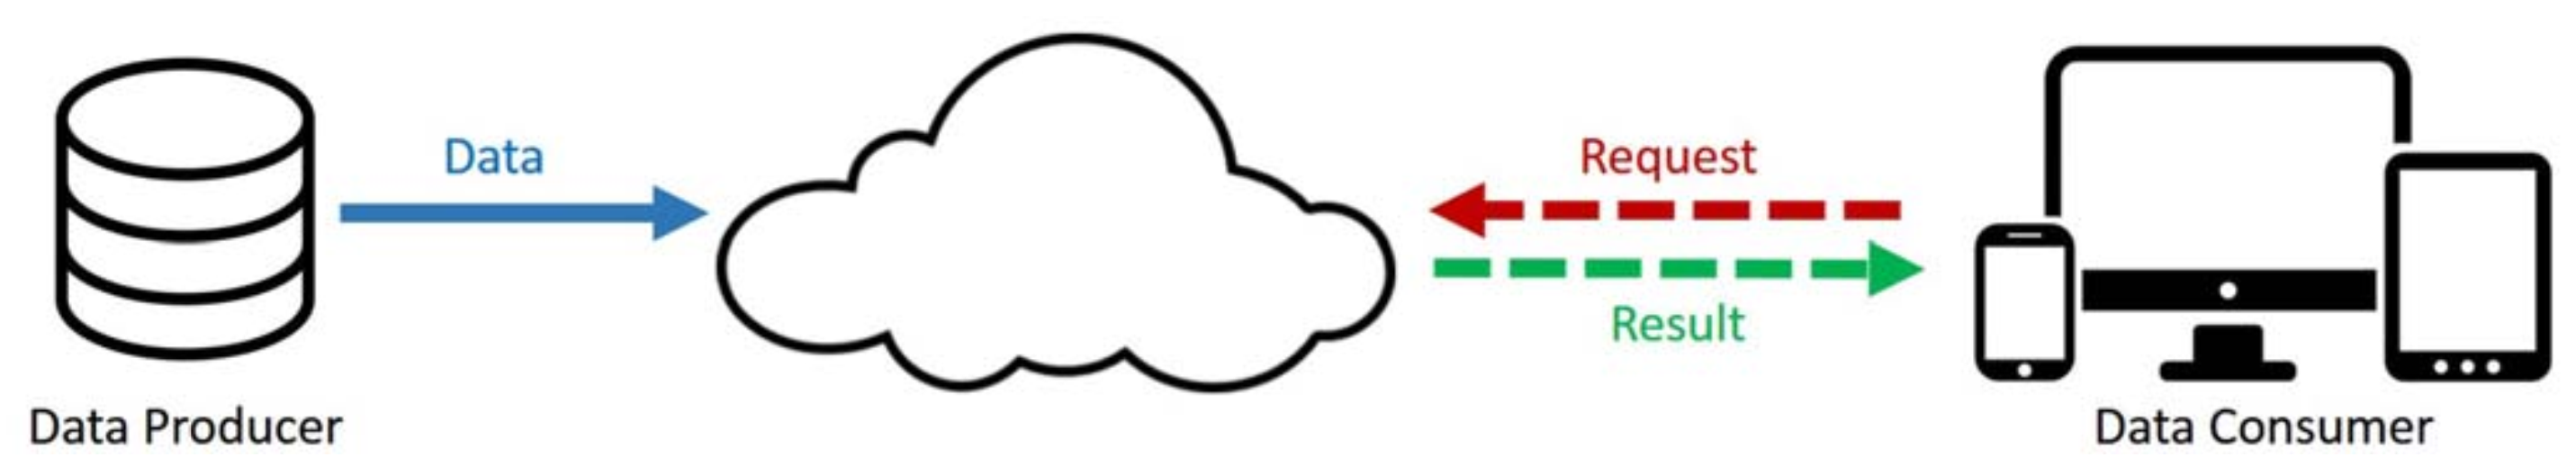
\includegraphics[width=10cm]{graphics/chapter_2/cloud_paradigm}}
            \caption{الگوی پردازش ابری \cite{shi2016edge}}
            \label{fig:chapter_2:cloud_paradigm}
          \end{figure}

        \item [تغییر از مصرف کننده داده به تولید کننده داده:]
          در الگوی پردازش ابری، دستگاه‌های انتهایی در لبه شبکه معمولا نقش مصرف کننده داده را دارند.
          به عنوان نمونه می‌توان تماشای یک ویدیو را مثال زد.
          با این حال امروزه مردم در حال تولید داده توسط دستگاه‌هایشان هستند.
          برای مثال امروزه بسیار عادی است که افراد عکس‌ها و ویدیو‌هایی که توسط خودشان ضبط شده است را در سرویس‌های اینترنتی مختلف به اشتراک بگذارند.
          در \cite{2019domo} اشاره شده است که در هر دقیقه در \lr{twitter} ۵۱۱۲۰۰ توییت جدید ارسال می‌شود و در \lr{instagram} ۵۵۱۴۰ عکس جدید بارگذاری می‌شود.
          باید توجه داشت که این تصاویر و ویدیوها می‌توانند حجم زیادی داشته باشند و پهنای باند زیادی را برای بارگذاری استفاده کنند.
          در این موارد ویدیو‌ها باید ابتدا حجمشان در لبه شبکه کاهش پیدا کند تا به وضوح تصویر\LTRfootnote{Resolution} مناسب برای بارگذاری در شبکه برسند.
          به عنوان نمونه‌ی دیگر می‌توان دستگاه‌های مربوط به سلامت را مثال زد.
          داده‌های جمع‌آوری شده توسط این دستگاه‌ها معمولا خصوصی است و پردازش این داده‌ها در لبه شبکه به جای ارسال داده‌ها برای پردازش به ابر به حفظ حریم خصوصی افراد کمک می‌کند.

      \end{description}
    
    \subsection{پردازش لبه چیست؟}
      پردازش لبه به همه تکنولوژی‌هایی اطلاق می‌شود که امکان انجام پردازش‌ داده‌ها در لبه شبکه را فراهم می‌کنند.
      در اینجا منظور از لبه، همه منابع پردازشی و شبکه ای است که بین منبع داده‌ها (جایی که داده‌ها در آن جا تولید می‌شوند) و مراکز داده‌ی ابری قرار دارند.
      برای مثال یک دروازه‌ی شبکه در یک خانه هوشمند، می‌تواند یک منبع پردازشی لبه بین اشیاء و مرکز داده‌ی ابری باشد یا یک مرکز داده‌ی کوچک، می‌تواند یک منبع پردازشی لبه بین دستگاه‌های سیار و ابر در نظر گرفته شود.
      منطق در پردازش لبه این است که پردازش داده‌ها باید در همسایگی منبع داده‌ها انجام شود.
      با این منطق پردازش لبه و پردازش مه دو مفهوم یکسان را خواهند داشت با این تفاوت که پردازش لبه تمرکزش سمت اشیاء است ولی پردازش مه تمرکزش سمت زیرساخت است.

      \begin{figure}[h]
        \centerline{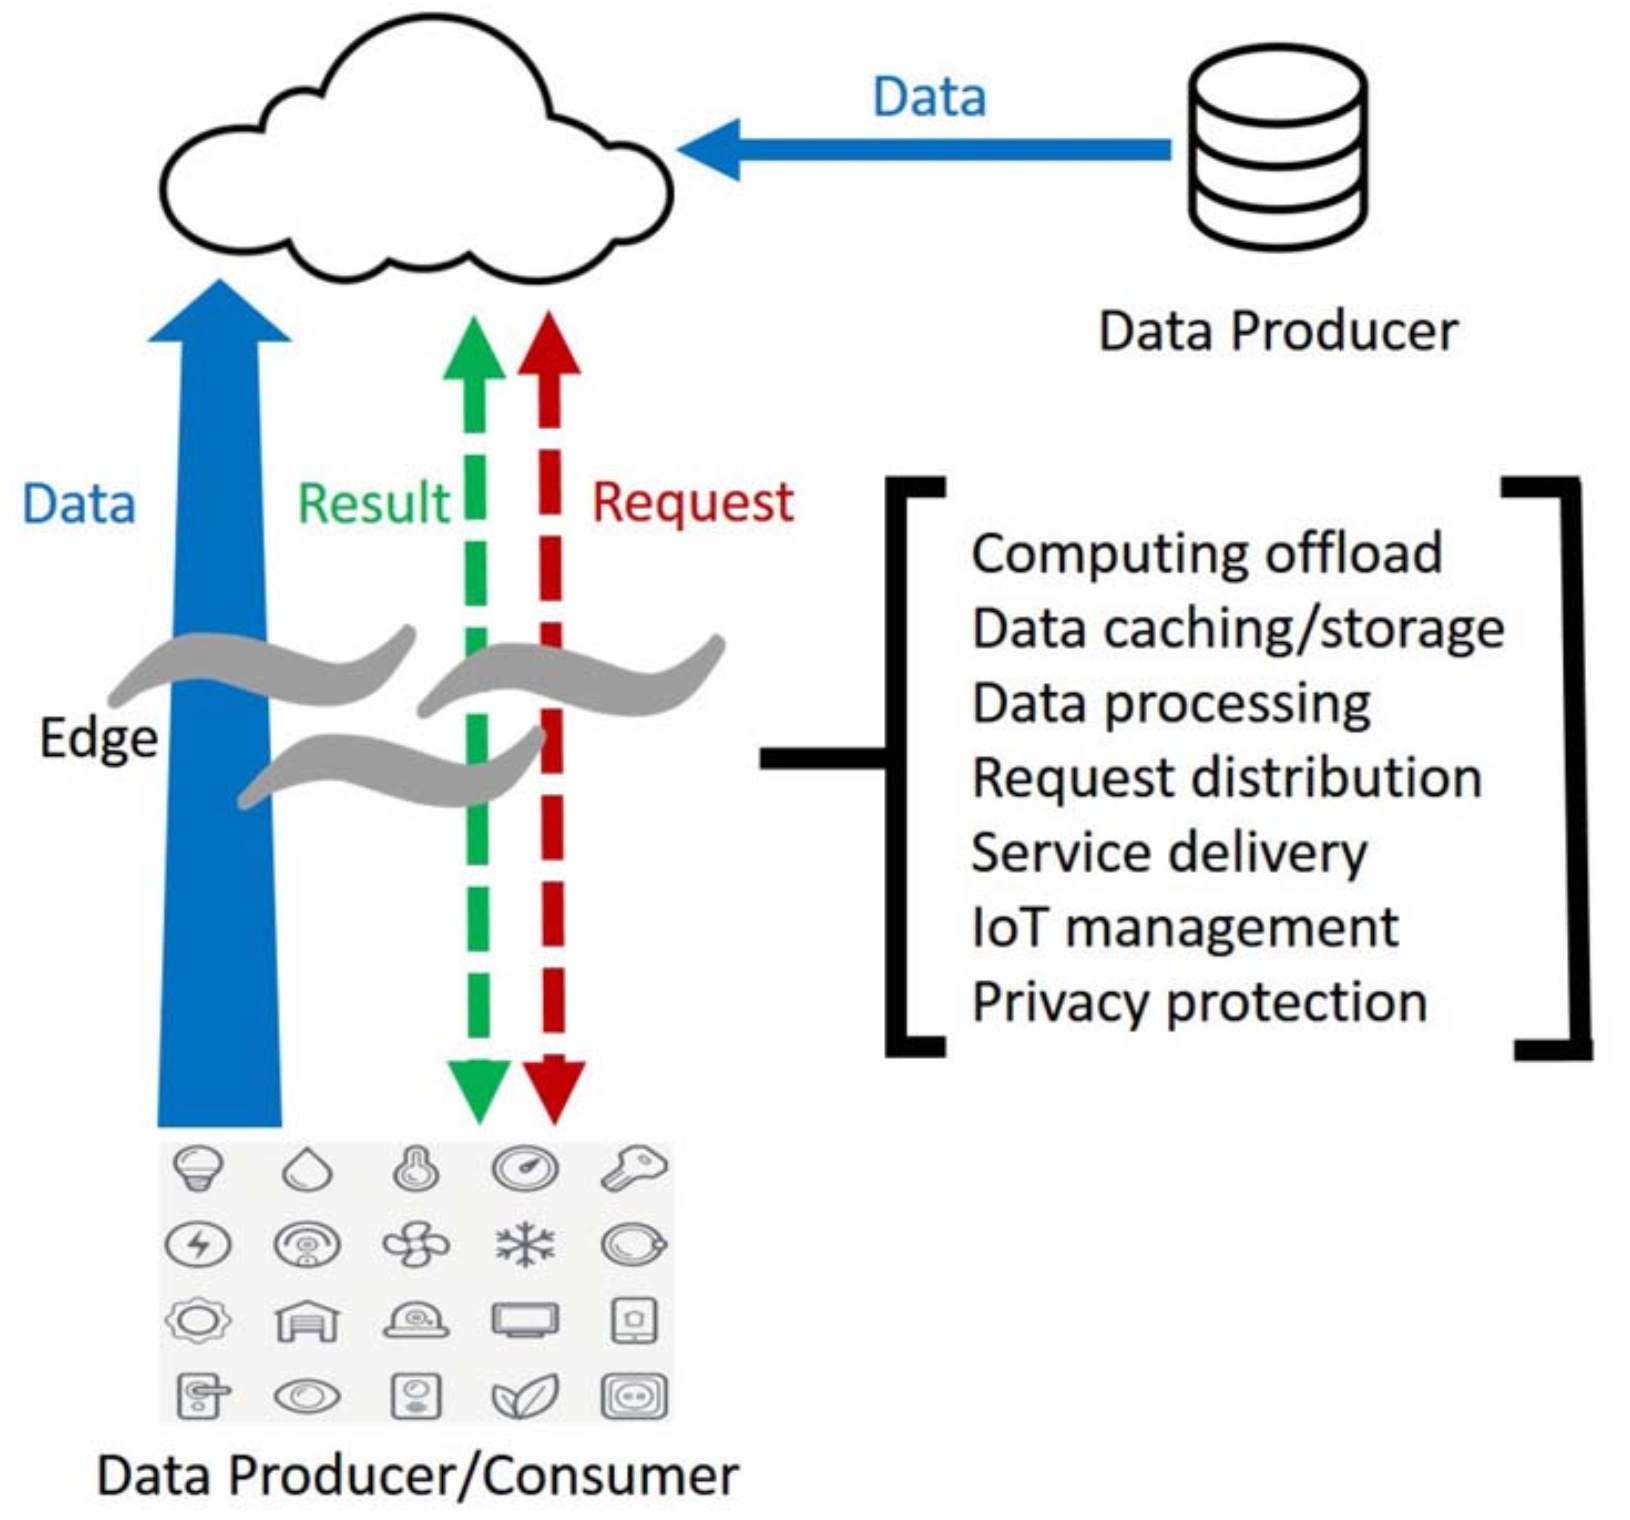
\includegraphics[width=10cm]{graphics/chapter_2/edge_paradigm}}
        \caption{الگوی پردازش لبه \cite{shi2016edge}}
        \label{fig:chapter_2:edge_paradigm}
      \end{figure}
      
      \cref{fig:chapter_2:edge_paradigm} جریان پردازش دو طرفه را در پردازش مه نشان می‌دهد.
      در الگو پردازش لبه، اشیاء نه تنها مصرف کننده داده بلکه تولید کننده‌ داده نیز هستند.
      در واقع در لبه، اشیاء نه تنها می‌توانند سرویس و محتوا از ابر درخواست نمایند بلکه می‌توانند وظایف پردازشی را هم انجام دهند.

    \subsection{مزایای پردازش لبه}
      همان طور که در بخش‌های قبل بیان شد، هدف از پردازش لبه قراردادن پردازش در مجاورت منبع تولید داده‌ها است.
      این کار مزایایی نسبت به روش‌های مبتنی بر پردازش ابری مرسوم دارد.
      در \cite{yi2015fog} برنامه‌ای برای تشخصی چهره ساخته شده است که با انتقال پردازش از ابر به لبه شبکه، زمان پاسخ برنامه از ۹۰۰ به ۱۶۰ میلی ثانیه کاهش پیدا کرده است.
      در \cite{ha2014towards} نویسندگان از واحدهای پردازشی ابری کوچک\LTRfootnote{Cloudlet} برای پردازش وظایف دستیار شناختی پوشیدنی\LTRfootnote{Wearable Cognetive Assitance} استفاده کرده اند و نتایج نشان می‌دهد که زمان پاسخ بین ۸۰ تا ۲۰۰ میلی ثانیه کاهش پیدا کرده است.
      روش ارائه شده در \cite{chun2011clonecloud} برای اجرای برنامه‌های تلفن همراه به کمک استفاده همزمان از پردازش ابری و پردازش لبه توانسته زمان اجرا و انرژی مصرفی را تا ۲۰ برابر کاهش دهد.

    \subsection{کاربرد پردازش لبه در شهر هوشمند}
      ویژگی‌های زیر باعث می‌شوند که پردازش لبه برای استفاده در شهر هوشمند مناسب باشد.
      \begin{enumerate}
        \item \textbf{حجم زیاد داده:}
          تخمین زده می‌شود که در سال ۲۰۱۹ میلادی یک شهر با جمعیت ۱ میلیون نفر، ۱۸۰ پتابایت داده در هر روز تولید می‌کند\cite{index2015forecast}.
          این داده‌ها توسط امنیت عمومی، سلامت، تجهیزات شهری و حمل و نقل تولید می‌شوند.
          ساختن مراکز داده‌ی متمرکز برای رسیدگی به همه‌ی این داده‌ها یک راهکار غیر واقعی است چرا که از این حجم از داده نیاز به قدرت پردازشی بسیار زیادی دارد.
          در این مورد پردازش لبه می‌تواند یک راه حل بهینه برای پردازش این حجم عظیم از داده‌ها باشد.

        \item \textbf{تاخیر کم:}
          برای کاربرد‌هایی که نیاز به تاخیر قابل پیشبینی و کم دارند مانند اورژانس سلامتی و امنیت عمومی، پردازش لبه یک الگوی مناسب است چرا که زمان انتقال داده‌ها را کاهش می‌دهد و ساختار شبکه را ساده‌تر می‌کند
        \item \textbf{آگاهی از مکان:}
          برای کاربرد‌های مبتنی بر موقعیت جغرافیایی مانند حمل و نقل و مدیریت تجهیزات شهری پردازش لبه به دلیل آگاهی از مکان، بهتر از پردازش ابری عمل می‌کند.
      \end{enumerate}

  \section{مجازی سازی}
    در الگوی پردازش ابری برای به اشتراک گذاری منابع از روش‌های مبتنی بر مجازی سازی\LTRfootnote{Virtualization} استفاده می‌شود و فراهم کننده‌های سرویس‌های زیرساخت ابری\LTRfootnote{Cloud Infrastructure as a Service Providers} به کمک این روش‌ها می‌تواند منابع را به صورت سریع به اشتراک بگذارد \cite{pahl2015containers} و \cite{jain2016overview}.
    در پردازش ابری ماشین‌های مجازی \LTRfootnote{Virtual Machine} به عنوان اصلی ترین روش مجازی سازی مورد استفاده قرار می‌گیرند.
    کارآمدی ماشین‌های مجازی در طول زمان با بهبود روش‌های زمان بندی، بسته بندی و ارتقاء امنیت آن‌ها بیشتر شده است.
    هر ماشین مجازی سیستم فایل بندی\LTRfootnote{File System} خود را به عنوان یک فایل مجزا روی حافظه کامپیوتر میزبان ذخیر می‌کند و به عنوان یک پردازه\LTRfootnote{Proccess} بزرگ در کامپیوتر میزبان اجرا می‌شود.
    برای حفظ امنیت هر کدام از این ماشین‌های مجازی، آن‌ها به صورت ایزوله نسبت به هم اجرا می‌شوند.

    در این روش مجازی سازی، هایپروایزر\LTRfootnote{Hypervisor} وظیفه مجازی‌سازی در سطح سخت افزار را دارد.
    به همین دلیل ماشین‌های مجازی از کامپیوتر میزبان مستقل خواهند بود.
    این استقلال از کامپیوتر میزبان باعث می‌شود که ماشین‌های مجازی با سیستم عامل متفاوت از سیستم عامل میزبان قابل اجرا باشند\cite{morabito2015hypervisors}.
    با این حال این روش دارای محدودیت‌هایی هم هست.
    یکی از این محدودیت‌ها این است که تصویر سیستم عامل میزبان به صورت کامل برای تک تک ماشین‌های مجازی نیاز است که باعث مصرف زیاد حافظه ذخیره‌سازی تصادفی و دیسک می‌شود.
    از دیگر محدودیت‌های این روش این است که شبیه سازی دستگاه‌های سخت افزاری توسط هایپروایزر باعث افزایش سربار پردازشی در کامپیوتر میزبان و کاهش بهره‌وری کلی می‌شود.
    علاوه بر این، این روش دارای زمان راه‌اندازی زیادی می‌باشد چراکه سیستم عامل تک تک ماشین‌های مجازی باید راه اندازی شود.
    از هایپروایزرهای مشهور می‌توان \lr{KVM (Kernel Based Virtual Machine)}\cite{2019kvm}, \lr{VMware ESXi}\cite{2019esxi}, \lr{Xen}\cite{2019xen} و \lr{Microsoft Hyper-V}\cite{2019hyper} نام برد.
    \cref{fig:chapter_2:vm} ساختار معماری مبتنی بر هایپروایزر را نشان می‌دهد.

    \begin{figure}[]
      \centerline{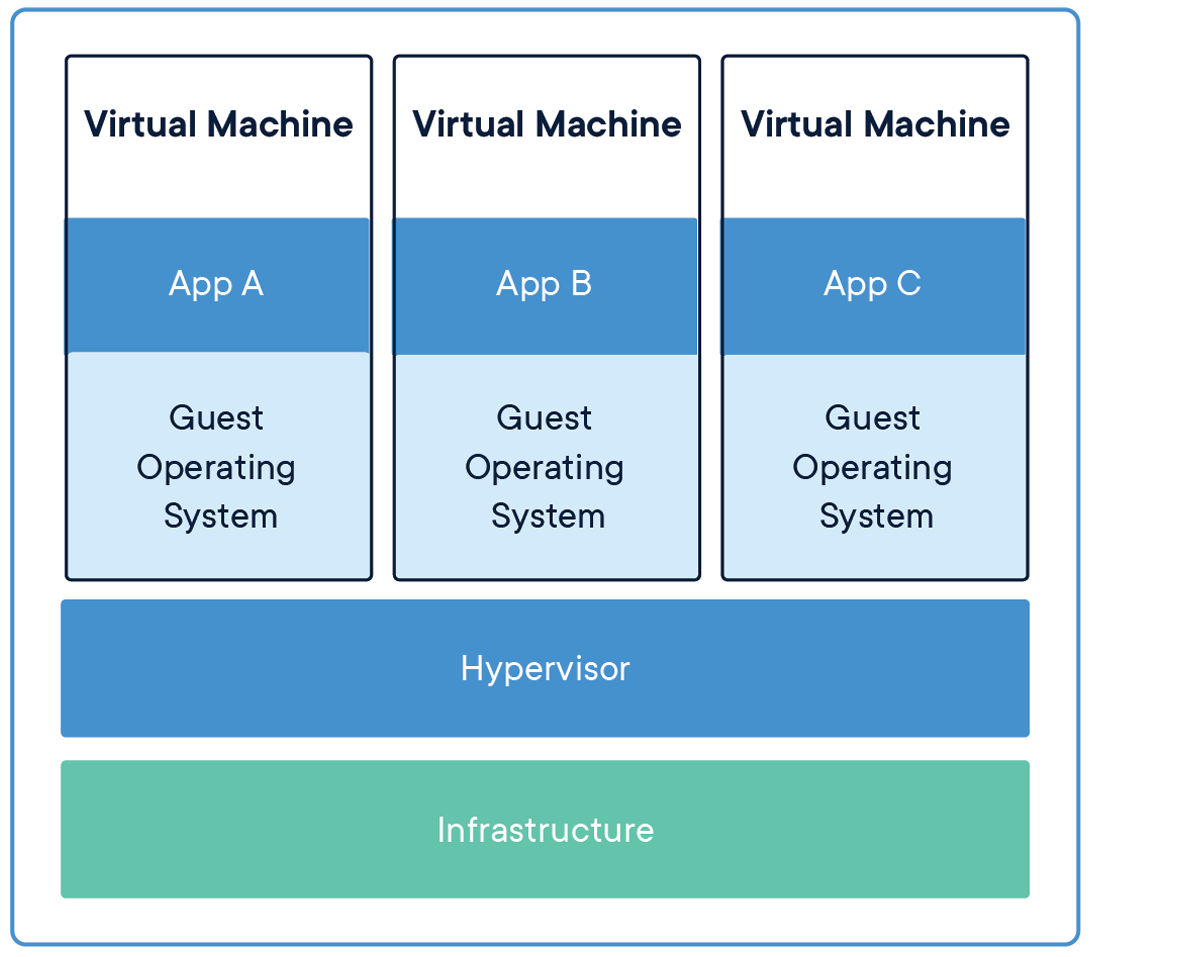
\includegraphics[width=10cm]{graphics/chapter_2/vm}}
      \caption{ساختار معماری مبتنی بر هایپروایزر \cite{2018are}}
      \label{fig:chapter_2:vm}
    \end{figure}

    روش‌های مجازی سازی مبتنی بر کانتینر\LTRfootnote{Container Based 
    Virtualization} مجازی سازی و ایزولاسیون را در سطی متفاوت از سطحی که روش‌های مبتنی بر هایپروایزر انجام می‌دهند، دنبال می‌کنند.
    درواقع می‌توان آن‌ها را جایگزین سبکی برای روش‌های مجازی سازی مبتنی برای هایپروایزر در نظر گرفت.
    در روش‌های مجازی سازی مبتنی بر هایپروایزر یک سیستم عامل مجزا به طور کامل برای هر کدام از ماشین‌های مجازی اجرا می‌شود.
    در مقابل در روش‌های مبتنی بر کانتینر، ایزولایسون پردازه‌ها در سطح سیستم عامل پیاده‌سازی می‌شود.
    برای این کار همه‌ی کانتینر‌ها بر روی یک سیستم عامل مشترک روی کامپیوتر میزبان اجرا می‌شوند و هر کانتینر می‌تواند شامل یک یا چند پردازه باشد.
    بنابراین سربار اجرای چندین سیستم عامل، راه‌انداز‌های سخت افزاری\LTRfootnote{Device Driver} و شبیه‌سازی سخت افزار‌های مختلف را از بین می‌برند.
    ساختار مجازی سازی مبتنی بر کانتیر در \cref{fig:chapter_2:container} نشان داده شده است.

    \begin{figure}[]
      \centerline{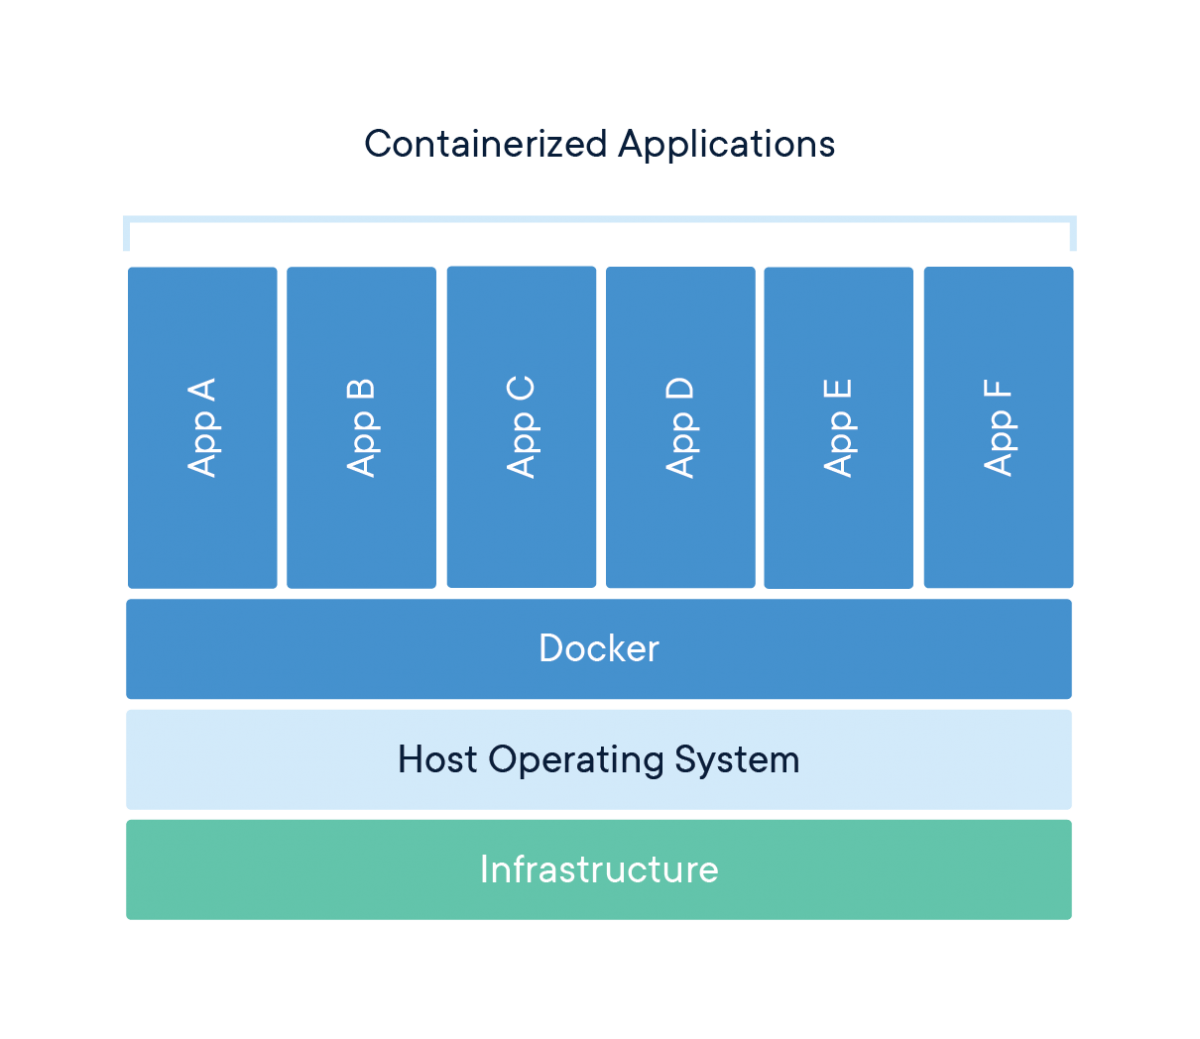
\includegraphics[width=10cm]{graphics/chapter_2/container}}
      \caption{ساختار مجازی سازی مبتنی بر کانتینر \cite{2018are}}
      \label{fig:chapter_2:container}
    \end{figure}
    
    مجازی سازی‌های مبتنی بر کانتینر در مقایسه با روش‌های مجازی سازی سخت افزاری مزایایی مانند سرعت ایجاد سریع‌تر دارند چرا که دیگر نیاز به شروع سیستم‌عامل جداگانه‌ای نیست.
    علاوه بر این سیستم‌های مبتنی بر کانتینر به دیلی حجم کم‌تر  تصویر‌ها\LTRfootnote{Image} و اجرا شدن روی هسته سیستم‌عامل\LTRfootnote{Operating System Kernel} مشترک می‌توانند تخصیص منابع بهتری داشته باشند \cite{morabito2015hypervisors}.

    با این حال استفاده از هسته‌ی سیستم عامل مشترک اشکالاتی در مقایسه با روش‌های مجازی‌سازی مبتنی بر هایپروایزر به همراه دارد.
    یکی از این اشکالات این است که کانتینر‌های سیستم عامل‌های مختلف قابل استفاده در سیستم عامل‌های دیگر نیستند.
    دیگر اشکال مجازی سازی‌های مبتنی بر کانتینر این است که ایزولاسیون در آن‌ها به خوبی روش‌های مجازی سازی مبتنی بر هایپروایزر نیست \cite{bui2015analysis} چرا که هسته سیستم عامل کامپیوتر میزبان در همه کانتینر‌ها مشترک است و این ممکن است برای امنیت در اجاره چندگانه\LTRfootnote{Multi-Tenant} مناسب نباشد.

    در ادامه به بررسی کانتینر‌ها در سیستم عامل لینوکس می‌پردازیم.
    در این سیستم عامل کانتینر‌ها به صورت عمده به وسیله‌ی گروه‌های کنترل\LTRfootnote{Control Groups (cgroups)}\cite{tejun2015Linux} و فضای نام‌ها\LTRfootnote{Name Spaces}\cite{2015Linux} پیاده‌سازی می‌شوند.

    گروه‌های کنترل در سال ۲۰۰۶ توسط مهندسان \lr{Google} توسعه داده‌شد و امکان مدیریت منابع مانند، محدودیت استفاده از منابع یا اولویت پردازه‌ها را برای گروهی از پردازه‌ها مشخص می‌کنند.
    فضای‌نام‌ها هم یک دید محدود و اختصاصی برای منابع سیستم در هر کانتینر ایجاد می‌کند.
    مجموعه‌ای از پردازه‌ها می‌توانند در یک فضای نام قرار بگیرند و محدودیت‌های یکسانی را در استفاده از منابع برای آن‌ها تعریف کرد.
    هر کامپیوتر می‌تواند چندید فضای نام داشته باشد و برای هر کدام ویژگی منابع توسط هسته‌ی سیستم عامل اعمال می‌شود.
    اختصاص منابع به هر فضای نام می‌تواند به گونه‌ای باشد که استفاده از واحد پردازنده مرکزی\LTRfootnote{Central Processing Unit (CPU)}، حافظه‌ی با دسترسی تصادفی\LTRfootnote{Random Access Memory (RAM)} و سایر منابع را برای مجموعه‌ای از پردازه‌ها محدود کند.
    با اضافه شدن ایزولاسیون گروه‌های کنترل در هسته لینوکس امکان ایجاد فضای نام‌هایی که از فضای نام‌های دیگر مستقل باشند ممکن شد.
    چند مورد از مهم‌ترین ویژگی‌های ایزولاسیون در فضای نام‌ها را ادامه بررسی می‌کنیم:
    \begin{enumerate}
      \item \textbf{فضای نام‌های شناسه پردازه‌ها\LTRfootnote{Process Identifier(PID)}:} این ویژگی باعث می‌شود که پردازه‌های یک فضای نام، از پردازه‌های فضای نام‌های دیگر با خبر نباشند.
      \item \textbf{فضای‌نام‌های شبکه:} ایزولاسیون کنترل‌کننده‌های رابط‌های‌ شبکه\LTRfootnote{Network Interface Controller (NIC)}، جدول‌های مسیریابی و ابزار‌های سطح پایین شبکه را ممکن می‌سازد
      \item \textbf{فضای نام‌های دستگاه‌های سوار شده\LTRfootnote{Mount Namespace}:} از این ویژگی برای ایزولاسیون دستگاه‌های سوار شده استفاده می‌شود که باعث می‌شود بتوان روی مصرف فضای نام‌های مختلف از دیسک محدودیت گذاشت.
      \item \textbf{فضای‌نام‌های کاربران:} کاربران یک فضای نام را به همان فضای نام محدود می‌کند و مانع تداخل شناسه‌های کاربری\LTRfootnote{User Identifier (UID)} یکسان در فضای نام‌های مختلف می‌شود.
    \end{enumerate}
    به بیان ساده‌تر این ویژگی‌ها باعث می‌شوند که هر فضای نام به عنوان کامپیوتر میزبان پردازه‌هایی که در آن اجرا می‌شوند ظاهر شود.

    از راه حل‌های مبتنی بر کانتینر می‌توان \lr{Linux-VServer}\cite{2019vserver}، \lr{OpenVZ}\cite{2019openvz}، \lr{LXC}\cite{2019containers}، \lr{Docker}\cite{2019docker} و \lr{rtk}\cite{2019rtk} را نام برد.
    در بین این راه‌حل‌ها \lr{LXC} و \lr{Docker} از بقیه مشهورتر هستند.
    \lr{LXC} یک راه حل سطح پایین‌تر ارائه می‌دهد و زمان زیادی است که موجود است.
    در واقع LXC اولین پیاده‌سازی چیزی که ما امروزه به نام کانتینر می‌شناسیم است.
    \lr{LXC} با استفاده از مزایای گروه‌های کنترل و فضای نام‌ها یک محیط مجازی درست می‌کند که پردازه‌ها به صورت جدا از هم اجرا می‌شوند.
    می‌توان این گونه برداشت کرد که \lr{LXC} امکان وجود فضا‌های کاربری\LTRfootnote{User Space} ایزوله و جدا را روی یک کامپیوتر فراهم می‌کند.
    در مقابل \lr{Docker} در سال ۲۰۰۹ معرفی شد و یک راه حل سطح بالاتر ارائه می‌دهد.
    \lr{Docker} با ترکیب کردن کانتینر‌های لینوکس با یک سیستم فایل‌بندی لایه‌لایه و ارائه ابزار‌هایی برای ساخت و بسته‌بندی برنامه‌های کاربردی به صورت تصویر کانتینر‌ها توانست محبوبیت زیادی کسب کند.
    نخستین نسخه‌های \lr{Docker} به صورت مستقیم از \lr{LXC} استفاده می‌کردند.
    در حال خاضر \lr{Docker} محبوب‌ترین تکنولوژی کانتینر می‌باشد به طوری که بیشتر افراد وقتی از تکنولوژی کانتینر نام برده می‌شود، فقط \lr{Docker} را در نظر می‌گیرند.
    با وجود تکنولوژی‌های مختلف کانتینر که در بالا اشاره شد، \lr{Docker} به عنوان یک استاندارد صنعتی برای کانتینر‌ها پذیرفته شده است.
    با این وجود داکر بر روی گروه‌های کنترل و فضای‌نام‌های هسته لینوکس بنا شده است.

    کانتینر‌های \lr{Docker} از چندین لایه از تصویر‌ها ساخته شده‌اند.
    این تصویر‌ها شامل فایل‌هایی دودویی هستند که باهم در یک بسته‌بندی قرار داده‌ شده‌اند.
    تصویر پایه سیستم عامل کانتینر را نگهداری می‌کند که می‌تواند متفاوت با سیستم عامل کامپیوتر باشد.
    سیستم عامل کانتینر، یک سیستم عامل کامل مانند سیستم عامل کامپیوتر میزبان نیست.
    تفاوت این است که تصویر تنها سیستم فایل بندی و فایل‌های دو دویی سیستم عامل را دارد ولی سیستم عامل کامپیوتر میزبان، سیستم فایل بندی، فایل‌های دو دویی و هسته سیستم عامل را دارا می‌باشد.
    روی تصویر پایه، چندین تصویر قرار می‌گیرد که هر کدام بخشی از کانتینر را می‌سازند.
    در واقع هر تغییری روی فایل‌های تصویر‌های قبلی باعث ایجاد یک لایه جدید می‌شود.
    مزیت این روش این است که باعث کاهش فضای لازم برای نگهداری تصویر کانتینر‌ها می‌شود.
    برای مثال دو کانتینر را با لایه‌های تصویر آ، ب و ث برای کانتینر اول و آ، ب و ت برای کانتینر دوم در نظر بگیرید.
    با این روش نگهداری، لایه‌های تصویر آ و ب تنها یکبار ذخیره می‌گردند ولی اگر تصویر‌ها یکپارچه بودند برای هرکانتینر باید فضا اشغال می‌کردند.

    \begin{figure}[]
      \centerline{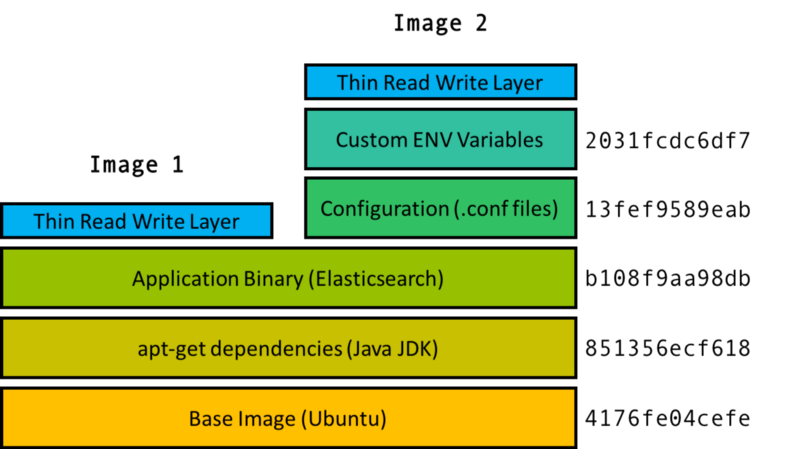
\includegraphics[width=10cm]{graphics/chapter_2/docker_image}}
      \caption{ساختار تصویر کانتینر‌ها در \lr{Docker} \cite{2019demystifying}}
      \label{fig:chapter_2:docker_image}
    \end{figure}

    در \lr{Docker} از نتیجه تابع در هم‌ساز\LTRfootnote{Hash} \lr{SHA-256} روی محتوای هر لایه به عنوان شناسه‌ی آن لایه‌ی تصویر استفاده می‌شود و هر لایه شناسه لایه‌های پایینی خود را نگهداری می‌کند و کانتینر‌ها با شناسه بالاترین تصویرشان متمایز می‌شوند.
    \cref{fig:chapter_2:docker_image}، ساختار تصویر دو کانتینر را نشان می‌دهد.
    همان طور که مشخص است این دو تصویر دارای سه لایه مشترک هستند و تصویر ۲ دارای دو لایه اضافی نیز هست.
    هنگامی که کانتینر اجرا می‌شود، \lr{Docker} ابتدا همه‌ی لایه‌های تصویر‌ها را بارگیری می‌کند.
    سپس گروه کنترل و نام‌دامنه‌های مربوط به کانتینر جدید را ایجاد می‌کند و از تصویر برای ایجاد محیط مجازی استفاده می‌کند به طوری که برای پردازه‌هایی که در آن کانتینر اجرا می‌شوند، انگار که فقط فایل‌های تصویر روی کامپیوتر قرار دارند.
    در انتها پردازه اصلی کانتینر را اجرا می‌کند.

    در \cite{ismail2015evaluation} نویسندگان، \lr{Docker} را به عنوان تکنولوژی که امکان استفاده از پردازش لبه را فراهم می‌کند بررسی کرده‌اند.
    نویسندگان، \lr{Docker} را در زمینه‌ی استقرار و پایان دادن سرویس‌ها، مدیریت منابع و سرویس‌ها، تحمل خطا و ذخیره‌سازی مورد بررسی قرار دادند و نتیجه گرفتند که \lr{Docker} به عنوان یک راه حل مناسب برای استفاده در پردازش لبه قابل استفاده است.
    در \cite{viswanath2016system} و \cite{morabito2016enabling} از تکنولوژی‌های مجازی‌سازی سبک برای طراحی دروازه‌های\LTRfootnote{Gateway} اینترنت اشیاء استفاده شده است.
    در \cite{viswanath2016system} از یک نرم‌افزار مجازی سازی برای استقرار انبوه سرویس‌ها در لبه شبکه استفاده کرده‌اند.
    نکته قابل توجه در تحلیل آن‌ها، امکان اثر متقابل بین حسگر‌های اینترنت اشیاء و دروازه‌‌ها می‌باشد.
    تحلیل آن‌ها نشان می‌دهد که تخصیص پویای سرویس‌ها با استفاده از کانتینر‌ها مزایایی از بعد کارایی در دروازه‌ها دارد.
    در \cite{morabito2016enabling} یک طراحی برای دروازه‌های اینترنت اشیاء ارائه شده است که می‌تواند به صورت بهینه در لبه شبکه استفاده شود.
    بررسی‌های انجام‌شده در این مقاله کارآمدی و انعطاف پذیری استفاده از \lr{Docker} را برای استفاده در یک سکوی‌ اینترنت اشیاء که سرویس‌های مجازی مختلفی مانند مدیریت دستگاه‌ها، پشتیبانی از شبکه‌های مبتنی بر نرم‌افزار\LTRfootnote{Software Defined Network (SDN)} و امکان مدیریت و ساماندهی داده‌ها را ارائه دهد، نشان می‌دهد.

    در \cite{novo2015capillary} از \lr{Docker} برای بسته‌بندی، استقرار و اجرای نرم‌افزار‌ها در ابر و دستگاه‌های با منابع محدود مانند دروازه‌های خاصی استفاده شده است.
    هدف این دروازه‌ها فراهم کردن اتصال شبکه‌های با برد کوتاه با شبکه‌های سلولی و فراهم کردن اجزاء نرم‌افزار‌های مختلف برای مدیریت دستگاه‌ها و پردازش‌های ابری توزیع‌شده می‌باشد.
    در \cite{celesti2016exploring} مجازی سازی مبتنی بر کانتینر و کامپیوتر‌های تک بردی\LTRfootnote{Single Board Computer (SBC)} به عنوان تکنولوژی‌هایی که امکان فراهم سازی سرویس‌های اینترنت اشیاء ابری را مهیّا می‌کنند، شناخته شده‌اند.
    مقاله \cite{krylovskiy2015internet} به شناسایی و بررسی نیازمندی‌های طراحی دروازه اینترنت اشیاء پرداخته است.
    نویسندگان کانتینر‌های \lr{Docker} را به عنوان تکنولوژی مناسب که این نیازمندی‌ها را برطرف می‌کند در نظر گرفتند.
    در این مطالعه، برای برآورد سربار لایه مجازی سازی از چند معیار ترکیبی و کاربردی استفاده شده است.
    با این حال، در این مطالعه، کارایی فقط برای برد \lr{Raspberry Pi} انجام شده و بررسی جامع مصرف توان و بهره‌وری انرژی در آن وجود ندارد.

    معماری ابر کوچک که در \cite{satyanarayanan2009case} معرفی شده است، یک روش کارآمد برای پردازش ابری سیار\LTRfootnote{Mobile Cloud Computing} ارائه می‌دهد که برخلاف مقالات قبلی از ماشین مجازی برای مجازی سازی استفاده کرده است.
    در \cite{pahl2016container} نویسندگان یک سکوی به عنوان سرویس\LTRfootnote{Platform as a Service (PaaS)} مبتنی بر کانتینر با استفاده از \lr{Raspberry Pi} معرفی کرده‌اند که در آن از تکنولوژی‌های کانتینری برای استفاده در معماری ابری لبه استفاده شده است.
    به طور مشابه در \cite{bellavista2017feasibility} از \lr{Docker} و \lr{Raspberry Pi} برای ایجاد یک شبکه پردازش لبه استفاده کرده‌اند.
    نویسندگان سربار استفاده از \lr{Docker} برای کامپیوتر‌های تک بردی را بررسی کرده و آن را ناچیز ارزیابی کرده‌اند.
    \cite{hajji2016understanding} به بررسی جزئی کارایی یک معماری ابری مبتنی بر \lr{Raspberry Pi} و \lr{Docker} برای استفاده در کاربرد‌های کلان داده\LTRfootnote{Big Data} می‌پردازد.
    در انتها، \cite{morabito2017virtualization} به بررسی کارآیی تکنولوژی‌های کانتینری روی کامپیوتر‌های تک بردی مختلف می‌پردازد.
    در همه این مقالات نتیجه گیری بر این است که با استفاده از کانتینر‌ها در دستگاه‌های مورد نظر، سربار پردازشی قابل چشم پوشی می‌باشد.

  \section{نو‌آوری‌های پایان نامه}
    دستاورد‌های این پایان‌نامه را می‌توان به صورت زیر خلاصه کرد:

    در بخش اول، برای صورت مسئله تخصیص منابع به صورت یک سرویس به یک منبع پردازشی، مدل ریاضی ارائه شده‌است و مسئله به صورت یک بهینه سازی نوشته شده‌است که هدف آن کمینه کردن مجموع هزینه سرویس‌ها است. برای حل این مسئله یک روش تخصیص منابع مبتنی بر مزایده استفاده است که امکان حل این مسئله به صورت موازی را دارد که برای شبکه‌های بزرگ مناسب است.

    در بخش دوم، برای صورت مسئله تخصیص منابع به صورت چند سرویس به چند منبع پردازشی، مدل ریاضی ارائه شده و به صورت یک مسئله بهینه سازی فرمول بندی شده که نرخ ارسال داده‌ی حسگر‌ها و بیشترین تاخیر سرویس را در تابع هزینه سرویس‌ها دخیل می‌کند و مجموع هزینه سرویس‌ها را کمینه می‌کند.
    ارائه الگوریتم برای حل این مسئله و بررسی تاثیر نرخ انتخابی در تاخیر سرویس‌ها از دیگر نو‌آوری‌های این پایان نامه است.

  \section{ساختار پایان‌نامه}
    ساختار پایان‌نامه به شرح زیر است.

    \cref{chap:literature_review} به مروری بر مطالعات انجام شده در زمینه تخصیص منابع اینترنت اشیاء می‌پردازد.

    \cref{chap:one_to_one_allocation} به بررسی مسئله اختصاص منابع پردازشی به صورت یک به یک در شبکه اینترنت اشیاء اختصاص دارد.
    در این فصل فرض بر این است که سرویس‌ها، می‌توانند از یک منبع پردازشی استفاده کنند و منابع پردازشی هم می‌توانند به یک سرویس اختصاص پیدا کنند.
    تخصیص منابع به صورت یک مسئله بهینه سازی فرمول بندی می‌شود که حل بهینه‌ی آن پیچیده است.
    برای حل مسئله از یک روش مبتنی بر مزایده استفاده شده که جواب قابل قبولی برای مسئله ارائه می‌دهد.

    در \cref{chap:many_to_many_allocation} مسئله تخصیص منابع پردازشی به صورت چند به چند در شبکه اینترنت اشیاء مورد بررسی قرار گرفته است.
    در این فصل بر خلاف فصل قبل منابع پردازشی می‌توانند به چند سرویس اختصاص پیدا کنند و سرویس‌ها هم می‌توانند از چند منبع پردازشی استفاده کنند.
    مانند فصل قبل مسئله تخصیص منابع به صورت یک مسئله بهینه سازی فرمول‌بندی شده است که حل بهینه پیچیده‌ای دارد و برای حل آن الگوریتمی پیشنهاد شده که در زمان کوتاه‌تری مسئله را حل می‌کند.

    در انتها در \cref{chap:conclusion} به بیان نتیجه‌گیری و کار‌های آینده می‌پردازیم.


\chapter{اختصاص منابع پردازشی در شبکه اینترنت اشیاء به صورت یک منبع پردازشی به یک سرویس}\label{chap:one_to_one_allocation}
  \thispagestyle{empty}
  \section{مقدمه}
    در این فصل ابتدا مدل ریاضی مربوط به تخصیص منابع پردازشی به صورت یک به یک در شبکه‌ی اینترنت اشیاء را شرح می‌دهیم. 
    در این نوع تخصیص منابع، تعدادی سرویس و منبع پردازشی داریم که سرویس‌ها باید برای پردازش داده‌های جمع‌آوری شده توسط حسگر‌های خود از منابع پردازشی موجود در شبکه استفاده کنند.
    یک به یک بودن در این نوع تخصیص منابع به این معنی است که هر سرویس حداکثر می‌تواند از یک منبع پردازشی استفاده کند و هر منبع پردازشی می‌تواند تنها پردازش لازم برای یک سرویس را انجام دهد.
    دستگاه‌هایی که دارای توان پردازشی بزرگی هستند، با استفاده از تکنولوژی کانتینر‌، توان پردازشی خود را به چند منبع پردازشی تقسیم می‌کنند و آن‌ها را به صورت جداگانه به اشتراک می‌گذارند.
    باید توجه کرد که، با توجه به توضیحات \cref{chap:literature_review} سربار پردازشی تقسیم قدرت پردازشی دستگاه‌ها، قابل نادیده گرفتن است.
    پس از معرفی و فرمول بندی مسئله، چالش‌ها و دلایل پیچیدگی حل این مسئله را بررسی می‌کنیم.
    سپس به معرفی راه‌حل مبتنی بر مزایده برای این مسئله می‌پردازیم.
  \section{مدل سیستم}
    \begin{figure}[h]
      \centerline{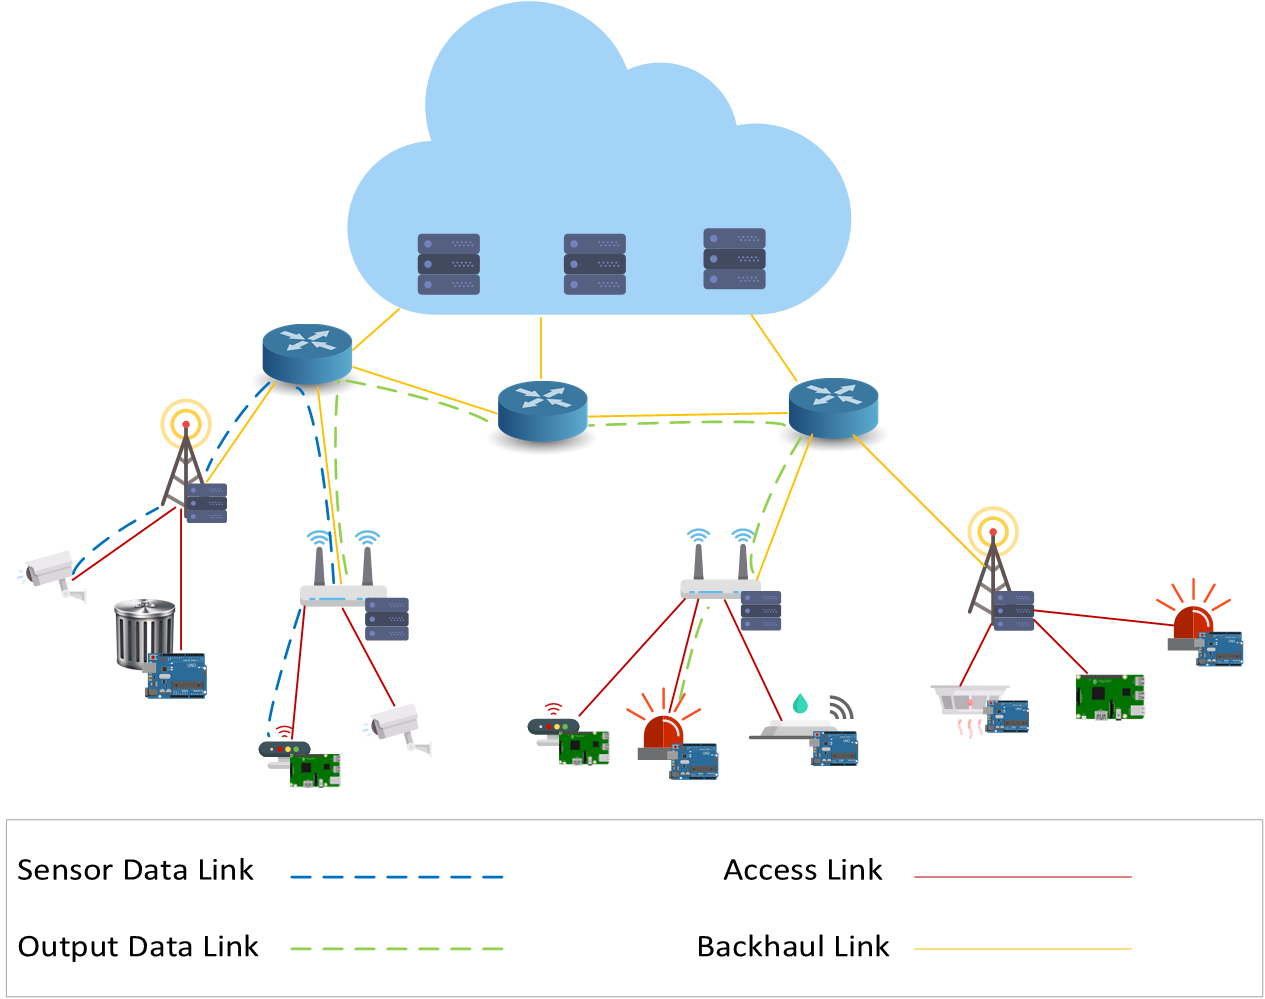
\includegraphics[width=12cm]{graphics/one_to_one/system_model}}
      \caption{دید کلی از مدل سیستم \cref{chap:one_to_one_allocation}}
      \label{fig:ono_to_one_system_model}
    \end{figure}

    \cref{fig:ono_to_one_system_model} مثالی از مدل سیستم این فصل را برای یک سرویس که دارای دو حسگر می‌باشد نشان می‌دهد.
    در یک منطقه جغرافیایی تعداد $N$ عدد سرویس و $M$ عدد فراهم کننده زیرساخت\LTRfootnote{Infrastructure Provider} پردازشی در نظر گرفته می‌شود.
    مجموعه سرویس‌ها را با $S$ و مجموع منابع پردازشی را با $C$ نمایش می‌دهیم.
    فراهم‌کننده‌های زیرساخت علاقه دارند که توان پردازشی اضافی خود را با دیگران به اشتراک بگذارند.
    در این فصل از $\phi_i$ برای بیان توان پردازشی فراهم‌کننده زیرساخت $i$ و از $\nu_i$ برای بیان درصدی از توان پردازشی که فراهم‌کننده زیرساخت پردازشی $i$ مایل به اشتراک‌گذاری آن است، استفاده می‌کنیم.
    در نتیجه، فراهم‌کننده زیرساخت پردازشی $i$ام، مایل به اشتراک‌گذاری توان پردازشی برابر با $\varphi_i = \phi_i \nu_i$ خواهد بود.
    در اینجا، گره‌های لبه\LTRfootnote{Edge Nodes}، گره‌هایی هستند که زیرساخت پردازشی را در لبه شبکه فراهم می‌کنند.
    در مقابل، فراهم‌کننده‌های زیرساخت ابری، منابع پردازشی را در فاصله‌ای دورتر از سرویس‌ها فراهم می‌کنند.
    بنابراین،‌ گره‌های لبه، توان پردازشی کم‌تر با تاخیر کم‌تر را در مقایسه با فراهم‌کننده‌های زیرساخت ابری مهیا می‌کنند.
    بده‌بستان\LTRfootnote{Trade-off}، بین میزان توان پردازشی و تاخیر در پردازش، باعث پیچیده‌شدن انتخاب گره‌های پردازشی برای سرویس‌ها می‌شود.
    
    \cref{tbl:one_to_one:notation} به صورت خلاصه پارامتر‌ها و متغیر‌های استفاده شده در این فصل را معرفی می‌کند.
    \begin{table}[h]
      \caption{نماد‌های استفاده شده در \cref{chap:one_to_one_allocation}}
      \begin{tabularx}{\textwidth}{|c|C|} \hline
        نشانه                & توضیح                                                                                     \\ \hline
        $N$                  & تعداد سرویس‌های شبکه                                                                       \\ \hline
        $M$                  & تعداد منابع پردازشی شبکه                                                                  \\ \hline
        $S$                  & مجموعه‌ی سریس‌های شبکه                                                                      \\ \hline
        $C$                  & مجموعه‌ی منابع پردازشی شبکه                                                                \\ \hline
        $d_{i,s}^\text{CPU}$ & تاخیر پردازشی سرویس $s$ در صورتی که از منبع پردازشی $i$ استفاده کند                       \\ \hline
        $d_{i,s}^\text{net}$ & تاخیر انتقال داده‌ها سرویس $s$  در صورتی که از منبع پردازشی $i$ استفاده کند                \\ \hline
        $\mu_{i,s}$         & نرخ سرویس منبع پردازشی $i$ برای سرویس $s$                                                  \\ \hline
        $r_s$               & نرخ انتخابی ارسال نمونه‌های سرویس $s$                                                       \\ \hline
        $R_s$               & نرخ مطلوب ارسال نمونه‌ها برای سرویس $s$                                                     \\ \hline
        $\omega_s$          & ضریب وزن دهی برای مشخص کردن نسبت اهمیت تاخیر نسبت به اختلاف نرخ انتخابی و نرخ مطلوب برای سرویس‌ها \\ \hline
        $\delta_{i,s}$      & متغیر دودویی که مشخص می‌کند سرویس $s$ منبع پردازشی $i$ را استفاده می‌کند یا خیر              \\ \hline
        $f_r$               & تابع مشخص کننده تاثیر اختلاف نرخ انتخابی با نرخ مطلوب در ارزش سرویس                         \\ \hline
        $f_d$               & تابع مشخص کننده تاثیر تاخیر در ارزش سرویس                                                  \\ \hline
        $U_{i,s}$           & ارزش سرویس $s$ در صورتی که از منبع پردازشی $i$ استفاده کند                                 \\ \hline
        $U_s$               & ارزش سرویس $s$                                                                             \\ \hline
        $U$                 & مجموع ارزش سرویس‌ها                                                                         \\ \hline
        $\eta$              & پارامتر محدود کننده‌ی بهره برداری از منابع پردازشی                                          \\ \hline
        $\epsilon$          & حداقل مقدار افزایش قیمت منابع پردازشی توسط سرویس‌ها در هر پیشنهاد                           \\ \hline
        $p_i$               & قیمت استفاده از منبع پردازشی $i$                                                           \\ \hline
        $\iota_s$           & منبع پردازشی با بیش‌ترین سود برای سرویس $s$                                                 \\ \hline
        $v_s$               & سود بهترین منبع پردازشی برای سرویس $s$                                                     \\ \hline
        $w_s$               & سود دومین بهترین منبع پردازشی برای سرویس $s$                                               \\ \hline
        $\gamma_s$          & میزان افزایش قیمت برای بهترین منبع پردازشی سرویس $s$                                       \\ \hline
      \end{tabularx}
      \label{tbl:one_to_one:notation}
    \end{table}

    در ابتدا تاخیر سرویس‌ها را بررسی می‌کنیم.
    تاخیر سرویس $s$ زمانی که از منبع پردازشی $i$ استفاده می‌کند، از دوبخش تشکیل می‌شود.
    یکی مربوط به تاخیر شبکه‌ است که آن را با $d^\text{net}$ نمایش می‌دهیم.
    دیگری مربوط به تاخیر پردازش است که آن را با $d^\text{CPU}$ نمایش می‌دهیم.
    تاخیر شبکه ،$d^\text{net}$، زمانی است که لازم است تا حسگر‌‌های یک سرویس داده‌ها را برای منبع پردازشی اختصاص یافته ارسال کنند به علاوه زمانی که لازم است تا گره پردازشی نتیجه را برای مقصد ارسال کند.
    تاخیر پردازشی ،$d^\text{CPU}$، زمانی است که طول می‌کشد تا داده‌ها در منبع پردازشی، پردازش شوند.
    
    در این‌جا فرض می‌کنیم که تاخیر شبکه ثابت است و تنها تابع فاصله جغرافیایی و ادوات شبکه بین فرستنده و گیرنده است.
    همانند \cite{optimial_price_cloud_valerio} از تئوری صف برای مدل کردن تاخیر پردازشی استفاده می‌کنیم.
    در این روش، پردازنده مانند یک سرویس دهنده عمل می‌کند و درخواست‌ها در یک صف قرار می‌گیرند تا نوبت پردازش آن‌ها فرار برسد.
    چون در این فصل هر گره پردازشی تنها به یک سرویس اختصاص پیدا می‌کند، از مدل $M/D/1$ استفاده می‌کنیم.
    در این مدل، فرایند ورود به صف بدون حافظه بوده و نرخ سرویس‌ مقدار ثابتی دارد.
    برای یک صف $M/D/1$ با نرخ ورود $\lambda$ و نرخ سرویس  $\mu$ میانگین تاخیر $\omega$ از رابطه زیر بدست می‌آید\cite{basic_queueing_sztrik}
    \begin{equation}\label{eqn:md1_queue_responsetime}
      \omega = \frac{1}{\mu} + \frac{\lambda}{2\mu(\mu-\lambda)}.
    \end{equation}
    
    نرخ ارسال نمونه‌های حسگر‌های سرویس $s$ را $r_s$ می‌نامیم.
    در صورتی که سرویس $s$ از منبع پردازشی $i$ استفاده کند نرخ ورود در مدل $M/D/1$ برای منبع پردازشی $i$ برابر $r_s$ خواهد بود.
    همان‌گونه که قبلا توضیح داده شد، $\varphi_i$ بیان‌گر ظرفیت پردازشی است که منبع پردازشی $i$ مایل به اشتراک گذاری آن است.
    این عدد در واقع تعداد دستور العمل‌های پردازنده مرکزی\LTRfootnote{CPU Instructions} که این منبع پردازشی در یک ثانیه می‌تواند اجرا کند را بیان می‌دارد.
    اگر فرض کنیم $F_s$ تعداد دستور العمل‌های لازم برای پایان یافتن پردازش‌های یک نمونه از داده‌های حسگر های سرویس‌ $s$ را نشان دهد، نرخ سرویس منبع پردازشی $i$ برای سرویس $s$ از رابطه زیر بدست می‌آید
    \begin{equation}
      \mu_{i,s} = \frac{\varphi_i}{F_s}.
    \end{equation}
    با جایگذاری این مقدار در \cref{eqn:md1_queue_responsetime} تاخیر پردازشی سرویس $s$ وقتی از منبع پردازشی $i$ استفاده می‌کند به صورت زیر دست می‌آید:
    \begin{equation}
      d_{i,s}^{\text{CPU}} = \frac{2\mu_{i,s}-r_s}{2\mu_{i,s}(\mu_{i,s}-r_s)}.
    \end{equation}

    در این جا فرض می کنیم که ارزش منبع پردازشی $i$ برای سرویس $s$ از دو بخش تشکیل شده است.
    بخش اول، تابع نرخ ارسال نمونه‌ها توسط حسگر‌های سرویس $s$ به منبع پردازشی $i$ است.
    این تابع را $f_r$ نام‌گذاری می‌کنیم و فرض می‌کنیم که $f_r$ تابعی از نرخ ارسال نمونه‌ها توسط حسگر‌های سرویس $s$ و نرخ مطلوب آن سرویس می‌باشد.
    در واقع $f_r$ بیان کننده‌ی تاثیر $r_s$ در ارزش بدست آمده از پردازش اطلاعات برای سرویس‌ها است.
    بخش دوم هم تابعی از تاخیر ایجاد شده (مجموع تاخیر شبکه و تاخیر پردازش) است که آن را با $f_d$ نمایش می‌دهیم.
    اگر فرض کنیم $R_s$ نرخ ارسال مطلوب نمونه‌ها برای سرویس $s$ و $r_s$ نرخ ارسال نمونه‌های سرویس $s$ باشد، ارزشی که سرویس $s$ با استفاده از منبع پردازشی $i$ بدست می‌آورد را به صورت زیر می‌توان نوشت
    \begin{equation}
      U_{i,s}(r_s) = \alpha_s \left (\omega_s f_r(r_s, R_s) + (1-\omega_s) f_d(d_{i,s}^{\text{net}} + d_{i,s}^{\text{CPU}}) \right ) .
    \end{equation}
    نکته قابل توجهه در این رابطه این است که $\omega_s \in [0,1]$ یک ضریب وزن دهنده است که تعیین کننده نسبت تاثیر $f_r$ به $f_d$ است.
    اگر $\omega = 1$ باشد ضریب $f_d$ صفر خواهد بود، در نتیجه تاخیر اثری در ارزش بدست‌آمده برای سرویس نقشی نخواهد داشت.
    اما $\omega = 0$ بیان‌گر این است که نرخ اختصاص یافته برای سرویس اهمیتی ندارد و فقط تاخیر برای سرویس مهم است.
    واضح است که اگر $\omega = 0$ باشد، نرخی که ارزشی بدست آمده برای سرویس را بیشینه می‌کند $r_s = 0$ است.
    در نتیجه $\omega = 0$ نتیجه قابل قبولی نخواهد داشت.
    $\alpha_s$ برای اثر دادن ارزش ذاتی سرویس‌ها است.
    پس $\alpha_s$ برای سرویس با ارزش بالاتر، باید مقدار بیشتری داشته باشد.
    در ادامه برای نشان دادن اختصاص منبع پردازشی $i$ به سرویس $s$ از $\delta_{i,s}$ که به صورت زیر تعریف می‌شود استفاده می‌کنیم
    \begin{equation*}
      \delta_{i,s} = 
      \begin{cases}
        1, & \text{اگر منبع پردازشی $i$ به سرویس $s$ اختصاص پیدا کرده باشد} \\
        0, & \text{در غیر این صورت}
      \end{cases}.
    \end{equation*}
    با این تعریف ارزش بدست آمده برای سرویس $s$ از تخصیص منابع را می‌توان به صورت زیر بیان کرد
    \begin{equation}
      U_{s} =  \alpha_s \left (\omega_s  f_r(r_s, R_s) + (1-\omega_s) \sum_{i=1}^M \delta_{i,s} f_d(d_{i,s}^{\text{net}} + d_{i,s}^{\text{CPU}}) \right).
    \end{equation}
    در این رابطه به دلیل ضرب $\delta_{i,s}$ در $f_d$ فقط $f_d$ مربوط به منبع پردازشی اختصاص یافته به سرویس $s$ در $U_s$ تاثیر گذار خواهد بود.

    هدف ما تخصیص منابع پردازشی است به طوری که مجموع ارزش بدست آمده برای سرویس‌ها را بیشینه شود.
    ارزشی که همه سرویس‌ها از تخصیص منابع بدست می‌آورند را $U$ نام‌گذاری می‌کنیم که به صورت زیر تعریف می‌شود
    \begin{equation}
      U = \sum_{s=1}^N \alpha_s \left (\omega_s f_r(r_s, R_s) + (1-\omega_s) \sum_{i=1}^M \delta_{i,s} f_d(d_{i,s}^{\text{net}} + d_{i,s}^{\text{CPU}}) \right).
    \end{equation}
    در واقع $U$ تابع هدف مسئله است و می‌توانیم مسئله تخصیص منابع را به صورت مسئله بهینه سازی زیر بنویسیم
    \begin{subequations}
      \begin{align}
        \underset{r_s, \delta_{i,s}}{\text{maximize}} \qquad & \sum_{s=1}^N \alpha_s \left (\omega_s f_r(r_s, R_s) + (1-\omega_s) \sum_{i=1}^M \delta_{i,s} f_d(d_{i,s}^{\text{net}} + d_{i,s}^{\text{CPU}}) \right ) \\
        \text{\lr{subject  to}} \qquad & \nonumber \\
        & 0 \le r_s, \forall s \in S\label{eqn:rate_positiveness} \\
        & r_s \le \eta \sum_{i=1}^M \mu_{i,s}, \forall s \in S\label{eqn:rate_saturation}\\
        & \sum_{s=1}^N \delta_{i,s} \le 1, \forall i \in C \label{eqn:one_to_one:resource_quota}\\
        & \sum_{i=1}^M \delta_{i,s} \le 1, \forall s \in S \label{eqn:one_to_one:service_quota}\\
        & \delta_{i,s} \in \{0, 1\}, \forall s \in S, i \in C
      \end{align}
    \end{subequations}
    قید \eqref{eqn:rate_positiveness} بیان می‌کند که نرخ ارسال انتخاب شده برای سرویس‌ها باید مثبت باشد.
    قید \eqref{eqn:rate_saturation} برای جلوگیری از اشباع شدن منابع پردازشی است.
    در این قید، $0 < \eta < 1$ حداکثر مقدار بهره‌برداری از منابع پردازشی اختصاص یافته به سرویس‌ها را محدود می‌کند.
    نکته حائز اهمیت این است که در صف‌های $M/D/1$ واریانس تاخیر با افزایش بهره‌برداری از منابع افزایش می‌یابد \cite{basic_queueing_sztrik}.
    به همین دلیل با افزایش $\eta$ واریانس تاخیر سرویس‌ها افزایش پیدا می‌کند که خود می‌تواند باعث افزایش نا اطمینانی در سرویس‌ها شود.
    در نتیجه ممکن برای بعضی سرویس‌ها لازم باشد که $\eta$ به طور جداگانه بر حسب نیازشان محاسبه شود.
    همان‌گونه که قبلا بیان شد در این فصل فرض بر این است که تخصیص منابع یک به یک است یعنی هر سرویس می‌تواند حداکثر از یک منبع پردازشی استفاده کند و هر منبع پردازشی هم حداکثر به یک سرویسی اختصاص پیدا می‌کند.
    قید‌های \eqref{eqn:one_to_one:resource_quota} و \eqref{eqn:one_to_one:service_quota} وظیفه دارند این شرایط را برقرار سازند.
        
    تابع‌های $f_r$ و $f_d$ در تابع هدف بهینه‌سازی باید شرایط خاصی داشته باشند تا بتوان آن‌ها را مورد قبول دانست.
    $f_r$ باید تابع اختلاف $r_s$ و $R_s$ باشد و با افزایش این اختلاف، مقدار آن کاهش پیدا کند.
    $f_d$ هم باید با افزایش تاخیر‌ کاهش پیدا کند.
    در ادامه‌ی این فصل فرض می‌کنیم:
    \begin{align}
      f_r(r_s, R_s) & = -|R_s - r_s| \label{eqn:one_to_one:f_r}\\
      f_d(d^\text{CPU}_{i,s} + d^\text{net}_{i,s}) & = - d^\text{CPU}_{i,s} - d^\text{net}_{i,s}
    \end{align}
    واضح است که این توابع، شرایطی که در بالا بیان شده است را دارند.

    مسئله بهینه سازی معرفی شده در این بخش یک مسئله برنامه‌ریزی غیرخطی عدد صحیح مخلوط \LTRfootnote{Mixed Integer Nonlinear Programming} می‌باشد.
    این نوع مسائل به طور کلی به سختی حل می‌شوند \cite{bertsimas1997introduction}.
    تعداد زیاد متغیر‌های موجود در این مسئله به دلیل تعداد فراوان سرویس‌ها و منابع پردازشی در سناریو‌های مربوط به اینترنت اشیاء پیدا کردن جواب بهینه این مسئله را غیر عملی می‌کنند.
    به همین دلیل یک جواب زیر بهینه که به صورت عملی قابل محاسبه باشد مطلوب است.
    در بخش بعدی روشی مبتنی بر مزایده را معرفی می‌کنیم که پاسخ زیر بهینه این مسئله را به صورت عملی محاسبه می‌کند.

  \section{تخصیص منابع با استفاده از مزایده}
    در روش‌ تخصیص منابع مبتنی بر مزایده فرض می‌شود که یک سرویس باید مقدار پول $p_i$ را به منبع $i$ بپردازد تا بتواند از آن استفاده کند.
    در این روش برای هر سرویس سود را اختلاف بین ارزشی که آن منبع برای سرویس ایجاد می‌کند و پولی که برای بدست آوردن آن پرداخت می‌کند، تعریف می‌کنیم.
    از این رو هرکدام از سرویس‌ها تلاش می‌کنند تا منبعی را بدست بیاورند که بیشترین سود را برای آن‌ فراهم می‌کند.
    باید توجه داشت که در این جا منظور از منابع، همان منابع پردازشی می‌باشد.
    \subsection{مروری بر روش مزایده}
      اگر $\iota_s$ منبعی باشد که بیشترین سود را برای سرویس $s$ فراهم کند، در این صورت رابطه زیر برای سرویس $s$ و منابع پردازشی برقرار خواهد بود:
      \begin{align}\label{eqn:maximal_net_value}
        U_{\iota_s,s}^* - p_{\iota_s} \ge \max_i \{U_{i,s}^* - p_i\}.
      \end{align}
      اگر \cref{eqn:maximal_net_value} برای همه سرویس‌ها برقرار باشد، به آن تعادل اقتصادی\LTRfootnote{Economic Equilibrium} می‌گویند\cite{auction_algorithms_bertsekas}.
      در این نوع تعادل، تمام طرف‌های درگیر، از منابع اختصاص یافته راضی هستند چرا که هیچکدام نمی‌توانند سود خود را افزایش دهند.
      در نتیجه هیچ‌کس انگیزه‌ای برای تغییر منابع اختصاص یافته ندارد.
      با این وجود، پیدا کردن این تعادل عملی نیست.
      دلیل عملی نبودن پیدا کردن این تعادل این است که حالت‌هایی وجود دارد که در فرایند پیدا کردن این تعادل حلقه به وجود می‌آید و فرایند خاتمه پیدا نمی‌کند.
      به عبارت دیگر حالت‌هایی ممکن است وجود داشته باشد که دو یا چند سرویس، ارزش یکسانی برای تعدادی از منابع قائل باشند.
      این حالت مانع افزایش قیمت منابع می‌شود.
      در نتیجه فرایند حراج هیچ وقت پایان نمی‌یابد.
      برای حل این مشکل، \cite{auction_algorithms_bertsekas} الگوریتمی ارائه کرد که تلاش می‌کند یک تعادل تقریبی\LTRfootnote{Almost Equilibrium} راپیدا کند.
      
      در یک تعادل تقریبی، تفاوت بین سود هریک از سرویس‌ها از بهینه بودن،باید حداکثر به اندازه‌ی $\epsilon$ باشد.
      در نتیجه در یک تعادل تقریبی رابطه زیر برای همه سرویس‌ها برقرار است
      \begin{equation}\label{eqn:almost_equilibrium}
        U_{\iota_s,s}^* - p_{\iota_s} \ge \max_i \{U_{i,s}^* - p_i\} - \epsilon.
      \end{equation}
      این رابطه برای هر سرویسی که برقرار باشد آن سرویس تقریبا راضی\LTRfootnote{Almost Happy} است.
      در واقع آن سرویس با تغییر منبعی که انتخاب کرده نمی‌تواند سود خود را بیشتر از $\epsilon$ افزایش دهد.
      این شرط با نام \lr{$\epsilon$ - complementary~slackness} شناخته می‌شود و در صورتی که $\epsilon = 0$ باشد، نتایج مانند تعادلی که توسط \cref{eqn:maximal_net_value} معرفی شد، خواهد داشت.
      الگوریتم معرفی شده، یک روش مبتنی بر تکرار است که بالاخره یک تعادل تقریبی را پیدا می‌کند.

      در ابتدا هرکدام از سرویس‌ها، منبع پردازشی که بیشترین سود را برایش فراهم می‌کند برمی‌گزیند.
      همان طور که قبلا هم بیان شد، $\iota_s$ بهترین منبع پردازشی را برای سرویس $s$ مشخص می‌کند.
      بنابراین رابطه زیر برای $\iota_s$ برقرار است:
      \begin{equation}\label{eqn:argmax_benefit}
        \iota_s = \argmax{i}\{U_{i,s}^* - p_i\}.
      \end{equation}
      سپس پیشنهاد دهنده (در این جا سرویس $s$) مبلغ پیشنهادی را برای منبع پردازشی $\iota_s$ به اندازه $\gamma_s$ بالا می‌برد
      \begin{equation}\label{eqn:bid_increase_1}
        \gamma_s = v_s - w_s + \epsilon,
      \end{equation}
      به طوری که $v_s$ بیشترین سودی است که سرویس $s$ می‌تواند بدست آورد
      \begin{equation}\label{eqn:bid_increase_2}
        v_s = \max_i\{U_{i,s}^* - p_i\},
      \end{equation}
      و $w_s$ بیشترین سودی است که سرویس $s$ بدست می‌آورد وقتی که $\iota_s$ از لیست منابع پردازشی حذف شود
      \begin{equation}\label{eqn:bid_increase_3}
        w_s = \max_{i \ne \iota_s}\{U_{i,s}^* - p_i\}.
      \end{equation}
      باید توجه کرد که $\gamma_s$ بیشترین مقداری است که قیمت منبع پردازشی $\iota_s$ می‌تواند افزایش پیدا کند به طوری که با اختصاص منبع پردازشی $\iota_s$ به سرویس $s$، آن سرویس تقریبا راضی باشد.
      بنابراین قیمت پیشنهادی جدید از رابطه زیر بدست می‌آید:
      \begin{equation}\label{eqn:bid_increase_4}
        p_{\iota_s} = p_{\iota_s} + \gamma_s.
      \end{equation}
      پس از این افزایش قیمت، سود بهترین منبع پردازشی (منبع پردازشی $\iota_s$) قبل از افزایش قیمت به اندازه‌ی $\epsilon$ کم‌تر از سود دومین منبع پردازشی قبل از افزایش قیمت خواهد بود.
      نکته‌ی قابل توجه در این افزایش قیمت این است که در حالتی که $\epsilon = 0$ باشد، پس از افزایش قیمت تفاوتی بین منبع پردازشی اول و منبع پردازشی دوم از لحاظ سود حاصل شده وجود ندارد.

      بعد از هر پیشنهاد قیمت، منبع پردازشی قیمت جدید را به همه اعلام می‌کند.
      در نتیجه سرویسی که قبلا بیشترین قیمت را پیشنهاد داده بود متوجه می‌شود که دیگر بیشترین پیشنهاد دهنده برای منبع پردازشی مربوطه نیست.
      این روش تاجایی ادامه پیدا می‌کند که قیمت منابع تاجایی بالا برود که فقط یک سرویس مایل به پرداخت آن قیمت برای بدست‌آوردن منبع پردازشی متناظر بشود.
      همان‌گونه که در \cite{auction_algorithms_bertsekas} بیان شده، $\gamma_s$ می‌تواند هر مقداری بزرگ‌تر از $\epsilon$ باشد ولی باید توجه داشت که مقادیر کوچکتر برای $\gamma_s$ موجب می‌شود که قیمت‌ها با قدم‌های کوچک‌تری در هر مرحله افزایش پیدا کنند.
      در نتیجه، افزایش قیمت پیشنهادی با میزانی کم‌تر از $\gamma_s$ باعث افزایش تعداد تکرار مراحل مزایده می‌شود.

    \subsection{معرفی الگوریتم تخصیص منابع مبتنی بر مزایده}
      در این جا از یک الگوریتم تکرار شونده برای اختصاص منابع پردازشی به سرویس‌ها استفاده می‌کنیم.
      در مرحله اول هر سرویس باید ارزشی که هر منبع پردازشی برایش دارد را محاسبه کند.
      برای این منظور باید نرخ بهینه ارسال اطلاعات را برای هر کدام از منابع پردازشی پیدا کند.
      فرض کنید $r_{i,s}^*$ نرخ بهینه برای سرویس $s$ وقتی از منبع پردازشی $i$ استفاده می‌کند باشد.
      در لم (\ref{lem:optimal_rate}) این نرخ بهینه را برای هر سرویس و هر منبع پردازشی پیدا می‌کنیم.
      اما ابتدا نیاز به لم زیر داریم.
      به کمک این لم می‌توانیم قدر مطلق را از \cref{eqn:one_to_one:f_r} حذف کنیم.
      \begin{lemma}\label{lem:optimal_rate_positive}
        برای سرویس $s$ وقتی از منبع پردازشی $i$ استفاده می‌کند, نرخ بهینه کم‌تر از $R_s$ است.
      \end{lemma}
      \begin{proof}
        برای اثبات از برهان خلف استفاده می‌کنیم.
        فرض کنید که $r_{i,s}^* \ge R_s$ نرخ بهینه سرویس $s$ وقتی از منبع پردازشی $i$ استفاده می‌کند باشد.
        باید توجه داشت که تابع ارزش هرکدام از منابع پردازشی برای سرویس‌ها ($U_{i,s}$) یک تابع نزولی نسبت به $r_{i,s}$ برای $r_{i,s} \ge R_s$ می‌باشد.
        چراکه هر دو بخش تشکیل دهنده این تابع برای $r_{i,s} \ge R_s$ با افزایش $r_{i,s}$ کاهش پیدا می‌کند.
        در نتیجه برای هر $\hat{r}_{i,s}$ به طوری که $r_{i,s}^* \ge \hat{r}_{i,s} \ge R_s$ رابطه $U(\hat{r}_{i,s}) \ge U(r_{i,s}^*)$ برقرار است که در تناقض با فرض اولیه است.
        در نتیجه نرخ بهینه کم‌تر از $R_s$ است.
      \end{proof}
      لم بعد، نرخ بهینه را برای سرویس $s$ وقتی از منبع پردازشی $i$ استفاده می‌کند را مشخص می‌کند.
      \begin{lemma}\label{lem:optimal_rate}
        اگر سرویس $s$ از منبع پردازشی $i$ استفاده کند نرخ بهینه از رابطه زیر بدست می‌آید:
        \begin{equation}\label{eqn:optimal_rate}
          r_{i,s}^* = \max\left\{0,\min\left\{R_s, \eta \mu_{i,s}, \mu_{i,s}-\frac{1}{2}\sqrt{2(1-\omega_s)/\omega_s}\right\}\right\}.
        \end{equation}
      \end{lemma}
      \begin{proof}
        با توجه به لم (\ref{lem:optimal_rate}) تابع ارزش منبع پردازشی $i$ برای سرویس $s$ با رابطه زیر قابل جایگزینی است:
        \begin{equation}
          (R_s - r_{i,s}) + \beta_s(d_{i,s}^{\text{net}} + d_{i,s}^{\text{cpu}}),
        \end{equation} 
        که در این رابطه $\beta_s=(1-\omega_s)/\omega_s$.
        این تابع یک تابع محدب است.
        پس برای پیدا کردن مقدار بهینه آن کافی است مشتق آن را مساوی صفر قرار دهیم و نتیجه را روی قید‌ها تصویر کنیم.
        \begin{align*}
          & \frac{\partial U_{i,s}}{\partial r_{i,s}} = 0 \\
          \Rightarrow &\frac{\partial}{\partial r_{i,s}}\{(R_s - r_{i,s}) + \beta_s(\sum_{i=1}^M d_{i,s}^{\text{net}} + d_{i,s}^{\text{cpu}})\} = 0 \\
          \Rightarrow & 1 + \beta_s[ \frac{1}{2\mu_{i,s}(\mu_{i,s}-r_{i,s}^*)} - \frac{2\mu_{i,s}-r_{i,s}^*}{2\mu_{i,s}(\mu_{i,s}-r_{i,s}^*)^2}] = 0 \\
          \Rightarrow & 2 {r_{i,s}^*}^2 - 4 \mu_{i,s} r_{i,s}^* + 2 \mu_{i,s}^2 - \beta_s = 0 \\
          \Rightarrow & r_{i,s}^* = \frac{4 \mu_{i,s} - \sqrt{16 \mu_{i,s}^2 - 8(2\mu_{i,s}^2 - \beta_s)}}{4} = \mu_{i,s} - \frac{\sqrt{2\beta_s}}{2}
        \end{align*}
        با تصویر کردن این رابطه روی قید‌های مسئله (\cref{eqn:rate_saturation,eqn:rate_positiveness}) به \cref{eqn:optimal_rate} می‌رسیم.
      \end{proof}  

      مراحل الگوریتم ارائه شده، در \cref{alg:one_to_one:auction} به صورت خلاصه بیان شده است.
      در ابتدا، هرکدام از منابع پردازشی، مقدار اولیه صفر را به عنوان قیمت برای خود انتخاب می‌کنند.
      سپس مراحل الگوریتم شروع می‌شود.
      در هر مرحله همه منابع کامپیوتری قیمت‌های خود را به سرویس‌ها اعلام می‌کنند.
      با استفاده از قیمت‌های اعلام شده هر سرویس بررسی می‌کند که هنوز بیشترین پیشنهاد را برای منبع پردازشی که در مرحله قبل انتخاب کرده دارد یا نه.
      اگر قیمت منبع پردازشی تغییر کرده بود یعنی دیگر بیشترین پیشنهاد را برای منبع پردازشی ندارد و باید منبع پردازشی و پیشنهاد جدید را دوباره انتخاب کند.
      برای این منظور با استفاده از \cref{eqn:argmax_benefit} و قیمت‌های جدید، منبع پردازشی با بیشترین سود را انتخاب می‌کند.
      سپس با استفاده از \crefrange{eqn:bid_increase_1}{eqn:bid_increase_4} قیمت پیشنهادی برای منبع پردازشی انتخاب شده را افزایش می‌دهد و آن را برای منبع پردازشی مربوطه ارسال می‌نماید.
      منابع پردازشی هم پس از دریافت پیشنهاد قیمت جدید، قیمت خود را به روزرسانی کرده و در مرحله بعد قیمت جدید را به اطلاع سرویس‌ها می‌رسانند.
      
      \begin{latin}
        \begin{algorithm}[tp]
          \caption{Auction ‌Based Resource Assignment Algorithm}
          \label{alg:one_to_one:auction}
          \begin{algorithmic}[1]
            \State{All computation resourcaes initialize their price with 0.} \label{state:auction_iteration:price_initialization}
            \While{There is atleast an unassigned service}
              \For {r in Computation Resources}
                \State{resource r broadcast its price to services}
              \EndFor
              \For {s in Services}
                \parState{Check the price of computation resource to see if the highest bidder of any resource. If not, change status to not assigned.} \label{state:service_iteration:check_assignment}
                \If{Not assigned to any computation resource}
                  \State{Find the computation resource having maximum benefit according to eq. \eqref{eqn:argmax_benefit}} \label{state:service_iteration:find_max}
                  \State{Compute new bid by using the eqs. \eqref{eqn:bid_increase_1} to \eqref{eqn:bid_increase_4}} \label{state:service_iteration:compute_new_bid}
                  \State{send the bid to the computation resource $I_s$} \label{state:service_iteration:send_bid}
                \EndIf
              \EndFor
              \For {r in Computation Resources}
                \If{received new bids}
                  \State{Update the price by the maximum bid.}
                \EndIf
              \EndFor
            \EndWhile
          \end{algorithmic}
        \end{algorithm}
      \end{latin}

    \subsection{بررسی هم‌گرایی}
      نویسنده در \cite{auction_algorithms_bertsekas} نشان داده که الگوریتم اختصاص منابع مبتنی بر مزایده بعد از تعداد محدودی تکرار، پایان می‌یابد.
      برای اثبات همگرایی باید توجه کرد که تا زمانی که سروریس‌ها به یک منبع پردازشی اختصاص پیدا کرده‌اند، تقریبا راضی هستند.
      واضح است که سرویس‌ها به محض بدست‌آوردن منبع پردازشی تقریبا راضی هستند چرا که منبع پردازشی را با این شرط انتخاب می‌کنند.
      همچنین سرویس‌ها تا زمانی که یک منبع پردازشی را در اختیار دارند هم تقریبا راضی هستند.
      دلیل این موضوع این است که قیمت منابع پردازشی در هر مرحله کاهش پیدا نمی‌کند (یا ثابت باقی می‌ماند یا افزایش پیدا می‌کند).
      در نتیجه سود منابع پردازشی برای سرویس‌ها هرگز افزایش پیدا نمی‌کند.
      تا زمانی که قیمت یک منبع پردازشی تغییر نکند، سرویس مربوطه آن را در اختیار دارد و سود بقیه منابع پردازشی هم هرگز افزایش پیدا نمی‌کند،‌ پس تا زمانی که سرویس مربوطه آن منبع پردازشی را در اختیار دارد، \cref{eqn:almost_equilibrium} برقرار است.

      از مطالبی که در بالا بیان شد می‌توان نتیجه گرفت که منابع پردازشی پس از دریافت اولین پیشنهاد در همه مراحل به یک سرویس اختصاص دارند و تا پایان مزایده، آزاد نمی‌شوند.
      همچنین در هنگام پایان مزایده \cref{eqn:almost_equilibrium} برای همه سرویس‌ها برقرار است.
      پس در پایان، سرویس‌ها در یک تعادل تقریبی قرار دارند.
      بنا بر این، در حالتی که $N<M$، وقتی که $N$ گره‌ی پردازشی پیشنهاد دریافت کنند، هرکدام از سرویس‌ها به یکی از گره‌های پردازشی اختصاص پیدا کرده‌اند.
      پس شرط پایان الگوریتم برقرار می‌شود و الگوریتم پایان می‌یابد.

      با توجه به \cref{eqn:bid_increase_1} در هر مرحله وقتی یکی از منابع پردازشی یک پیشنهاد دریافت می‌کند، قیمتش حداقل به اندازه $\epsilon$ افزایش پیدا می‌کند.
      پس می‌توان نتیجه گرفت که پس از $m$ بار دریافت پیشنهاد جدید، قیمت منبع پردازشی مربوطه حداقل به اندازه‌ی $m\epsilon$ افزایش پیدا کرده است.
      برای مقادیر $m$ به اندازه کافی بزرگ، قیمت منبع پردازشی به اندازه‌ای افزایش پیدا کرده است که بعضی از سرویس‌ها پیشنهاد دادن به آن را متوقف کنند و شروع به پیشنهاد دادن به منابع پردازشی دیگر بکنند.
      همان طور که در بالا بیان شد وقتی این افزایش قیمت‌ها باعث شود که به $N$ منبع پردازشی پیشنهاد داده شود، الگوریتم پایان می‌یابد.
    \subsection{بررسی بهینگی الگوریتم}
      در \cite{distributed_auction_algorithms_zavlanos} نویسندگان ثابت کرده‌اند که نتیجه این الگوریتم حداکثر در فاصله $N\epsilon$ از مقدار بهینه قرار دارد.
      اگر $\alpha$ نشان دهنده نگاشت بین سرویس‌ها و گره‌های پردازشی باشد به طوری که $\alpha: \{1, \hdots, N\} \rightarrow \{1, \hdots, M\}$ , $\alpha(i) = \alpha_i$ آنگاه رابطه زیر برقرار است:
      \begin{equation}\label{eqn:auction_optimality_1}
        \sum_{i=1}^N U_{i,\alpha(i)}^* - \sum_{j=1}^M p_j \le \sum_{i=1}^N U_{i,\alpha(i)}^* - p_{\alpha(i)}.
      \end{equation}
      هم‌چنین واضح است که رابطه زیر برقرار است:
      \begin{equation}\label{eqn:auction_optimality_2}
        \sum_{i=1}^N U_{i,\alpha(i)}^* - p_{\alpha(i)} \le \sum_{i=1}^N \max_j\{U_{i,j}^* - p_j\}.
      \end{equation}
      با استفاده از \cref{eqn:auction_optimality_1,eqn:auction_optimality_2} می‌توان به رابطه زیر رسید:
      \begin{equation}\label{eqn:auction_optimality_3}
        \sum_{i=1}^N U_{i,\alpha(i)}^* \le \sum_{j=1}^M p_j + \sum_{i=1}^N \max_j\{U_{i,j}^* - p_j\}.
      \end{equation}
      تاکید می‌شود که \cref{eqn:auction_optimality_3} برای همه‌ی $\alpha \in \{1,\hdots,M\}$ و همه‌ی مجموعه قیمت‌های $\{p_j\}_{j=1}^M$ برقرار است.
      اگر مجموع ارزش حاصل از تخصیص منابع بهینه را $A^*$ بنامیم، برای $A^*$ رابطه زیر برقرار است:
      \begin{equation}\label{eqn:auction_optimality_A_defenition}
        A^* \triangleq \max_{\alpha(i),~i=1, \hdots, N} \sum_{i=1}^N U_{i, \alpha(i)}^*.
      \end{equation}
      اگر $D^*$ را به صورت زیر تعریف ‌کنیم:
      \begin{equation}\label{eqn:auction_optimality_D_defenition}
        D^* \triangleq \min_{p_j,~j=\{1, \hdots, m\}} \sum_{j=1}^M p_j + \sum_{i=1}^N \max_j\{U_{i,j}^* - p_j\}،
      \end{equation}
      آن‌گاه با توجه به \cref{eqn:auction_optimality_3} می‌توان نتیجه گرفت که $A^*<D^*$ است.
      
      همان‌طور که گفته شد در هنگامی که الگوریتم مزایده به پایان می‌رسد، تخصیص منابع و قیمت‌های حاصل شده از الگوریتم، در تعادل تقریبی قرار دارند.
      اگر $\hat \alpha$ را تخصیص منابع حاصل از الگوریتم در نظر بگیریم، \cref{eqn:almost_equilibrium} را می‌توان به صورت زیر باز‌نویسی کرد:
      \begin{equation}\label{eqn:auction_almost_equilibrium2}
        U_{i, \hat \alpha(i)}^* - p_{\hat \alpha(i)} \ge \max_j \{U_{i,j}^*-p_j\}-\epsilon.
      \end{equation}
      از این رو می‌توان نتیجه گرفت که
      \begin{align}
        D^* & \le \sum_{i=1}^N \left(p_{\hat \alpha (i)}+\max_j\{U_{i,j}^*-p_j\}\right) \\
            & \le \sum_{i=1}^N U_{i, \hat \alpha (i)}^* + N \epsilon \label{eqn:auction_D_upper_bound}.
      \end{align}

      از این که $A^* \le D^*$ و \cref{eqn:auction_D_upper_bound} می‌توان نتیجه گرفت که
      \begin{equation}
        A^* - N \epsilon \le \sum_{i=1}^N U_{i, \hat \alpha (i)}^*.
      \end{equation}
      این رابطه بیان کننده یک حد پایین برای مجموع ارزش منابع اختصاص یافته توسط اگوریتم مزایده می‌باشد.
      درواقع این رابطه بیان می‌کند که نتیجه حداکثر در فاصله $N \epsilon$ مقدار بیشینه قرار دارد.
    \subsection{بررسی پیچیدگی الگوریتم}
      نویسندگان در \cite{distributed_auction_algorithms_zavlanos} پیچیدگی الگوریتم مزایده را بررسی کرده‌اند.
      برای بررسی پیچیدگی الگوریتم مزایده، بدترین حالت را در نظر می‌گیریم که در آن تمام سرویس‌ها قیمت پیشنهادی را در هر مرحله به اندازه $\epsilon > 0$ افزایش می‌دهند (تا جایی که منبع پردازشی برایشان جذاب نباشد).
      برای این منظور، فرض کنید $\delta > 0$ و $T_j>0$ و رابطه زیر برای $U_{i,j}^*, j=1,\hdots,M$ برقرار باشد
      \begin{gather}
        \max_i U_{i,j}^* - \min_i U_{i,j}^* < \delta \\
        \min_i U_{i,j}^* - \max_i U_{i,(j-1)}^* = T_j
      \end{gather}
      فرض کنید منبع پردازشی $N$ در ابتدا جذاب‌ترین منبع برای همه‌ی سرویس‌ها باشد.
      اگر $\delta$ به اندازه‌ی کافی کوچک باشد، قیمت آن باید حداقل به اندازه‌ی $T_N$ افزایش پیدا کند تا دیگر تنها منبع پردازشی جذاب نباشد.
      این مقدار افزایش قیمت نیاز به $\lceil T_N / \epsilon \rceil$ پیشنهاد توسط هر سرویس دارد.
      در نتیجه $N \lceil T_N / \epsilon \rceil$ تکرار طول می‌کشد تا دومین منبع پردازشی هم برای سرویس‌ها جذاب شود.
      حال که دو منبع پردازشی جذاب برای سرویس‌ها وجود دارد، هر سرویس باید $2 \lceil T_{N-1} / \epsilon \rceil$ پیشنهاد بدهد تا قیمت این دو منبع پردازشی به اندازه‌ای افزایش پیدا کند که منبع پردازشی سوم هم برای سرویس‌ها جذاب شود.
      واضح است این کار نیاز به $2N \lceil T_{N-1} / \epsilon \rceil$ تکرار الگوریتم دارد.
      به همین ترتیب می‌توان نتیجه گرفت که منبع پردازشی $N-k+1$ نیاز به $kN \lceil T_{N-k+1} / \epsilon \rceil$ تکرار الگوریتم دارد.
      با توجه به این که الگوریتم زمانی پایان خواهد یافت که حداقل $N$ منبع پردازشی پیشنهاد دریافت کنند، رابطه زیر را برای تعداد تکرار‌های الگوریتم می‌توان نوشت
      \begin{equation}
        N\sum_{k=1}^N k \left \lceil \frac{T_{N+k-1}}{\epsilon} \right\rceil < N ^ 2 \left \lceil \frac{\max_{i,j} \{U_{i,j}^*\} - \min_{i,j} \{U_{i,j}^*\}}{\epsilon} \right\rceil.
      \end{equation}
  \section{نتایج شبیه‌سازی}
    در این قسمت نتایج شبیه‌سازی را بیان می‌کنیم.
    در همه موارد شبیه‌سازی برای ۲۰۰ بار اجرا شده و نتایج میانگین آورده شده‌اند.
    یک شبکه با تعداد $N$ سرویس و $M$ منبع پردازشی که در داخل یک دایره به شعاع $R=\text{\lr{1Km}}$ به صورت تصادفی پراکنده ‌شده‌اند را در نظر می‌گیریم.
    برای هر سرویس عددی در بازه $[1,10]$ برای تعداد مقصد‌ها و در بازه $[1,5]$ برای تعداد منبع‌ها به صورت تصادفی در نظر می‌گیریم و فرض می‌کنیم منبع‌ها و مقصد‌های سرویس‌ها به صورت تصادفی در شعاع $20m$ از نقطه‌ی انتخاب شده برای سرویس پخش شده‌اند.
    فرض می‌کنیم شبکه از تعدادی دستگاه مسیریابی که به صورت سلسله مراتبی سازمان یافته اند،‌تشکل شده‌است.
    هر کدام از این دستگاه‌های مسیر‌یابی از نزدیک ترین دستگاه مسیریابی سطح بالاتر برای اتصال به شبکه استفاده می‌کند و دستگاه‌های مسیر یابی در بالاترین لایه با توپولوژی مش به هم متصل هستند.
    مبدأ‌ها و مقصدهای سرویس‌ها و منابع پردازشی که در لبه شبکه قرار دارند از نزدیک‌ترین مسیریاب در پایین ترین لایه استفاده می‌کنند.
    در مقابل، منابع پردازشی ابری از نزدیک‌ترین مسیریاب در بالاترین لایه استفاده می‌کنند.
    برای تاخیر مسیریاب‌ها فرض می‌کنیم که به صورت میانگین عبور بسته‌ها از مسیریاب‌های لایه ۱، ۱ میلی ثانیه، مسیریاب‌های لایه ۲، ۲ میلی ثانیه و مسیریاب‌های لایه ۳، ۳ میلی ثانیه طول می‌کشد.
    \cref{fig:network} توپولوژی شبکه را که در شبیه‌سازی استفاده شده‌است نشان می‌دهد.
    
    \begin{figure}[h]
      \centerline{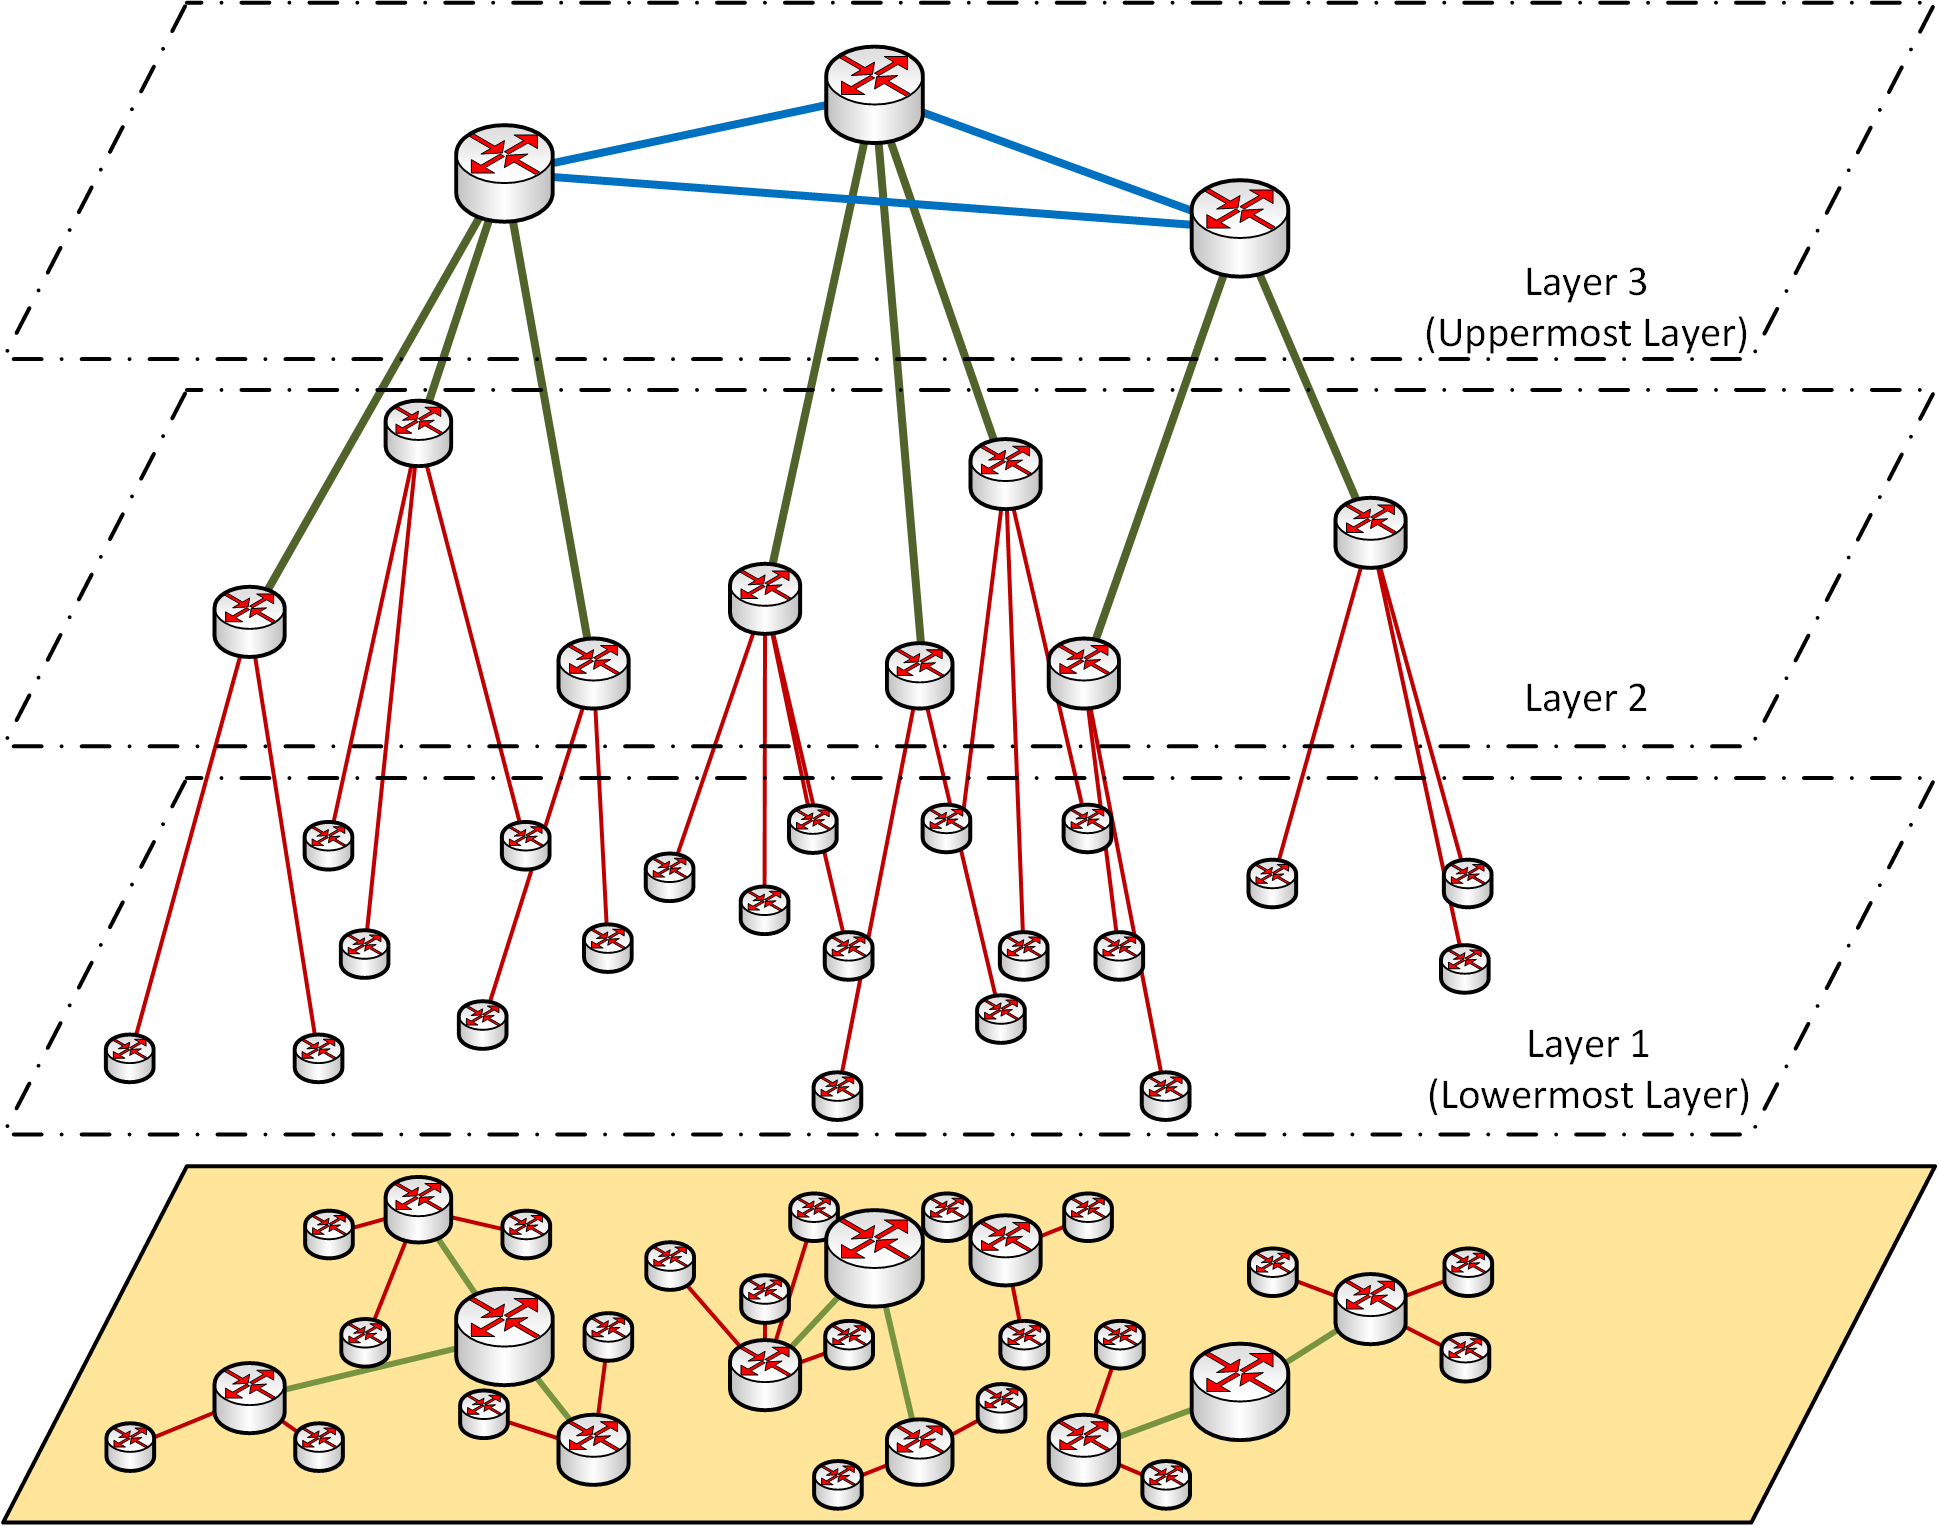
\includegraphics[width=15cm]{graphics/one_to_one/network}}
      \caption{دید کلی از توپولوژی شبکه}
      \label{fig:network}
    \end{figure}

    برای مقدار $\eta$ هم ۰٫۹ را در نظر می‌گیریم و فرض می‌کنیم ظرفیت پردازشی منابع پردازشی لبه شبکه به صورت تصادفی در محدوده‌ی $[1200, 1400]$ توزیع شده‌اند.
    برای ظرفیت پردازشی منابع پردازشی ابری هم مقدار ثابت $1000$ را در نظر می‌گیریم.
    علاوه بر این $\alpha_s$ به صورت تصادفی در بازه $[1, 10]$ توزیع شده است.
    در این فصل، برای هر سرویس تاخیر در حدود چند میلی ثانیه خواهد بود.
    در نتیجه برای رسیدن به نتایج معنی دار فرض می‌کنیم که $\beta_s = (1-\omega_s)/\omega_s$ به صورت یکنواخت در بازه $[30,70]$ توزیع شده اند.
    
    فرض می‌کنیم که تعداد سرویس‌ها $N=300$ باشد و تعداد منابع پردازشی لبه شبکه ($M$) از ۳۹۰ تا ۱۰۰۰ تغییر کند.
    در این قسمت هزینه سرویس $s$ را $-U_s$ تعریف می‌کنیم. 
    در نتیجه میانگین هزینه سرویس‌ها برابر خواهد بود با $-U/N$.
    دو سناریو را در نظر می‌گیریم.
    در سناریو‌ی اول فرض می‌کنیم که فقط منابع پردازشی لبه شبکه وجود دارند ولی در سناریو دوم یک فراهم کننده ابری با ۴۰ منبع پردازشی هم در شبکه حضور دارد.
    
    \begin{figure}
      \centerline{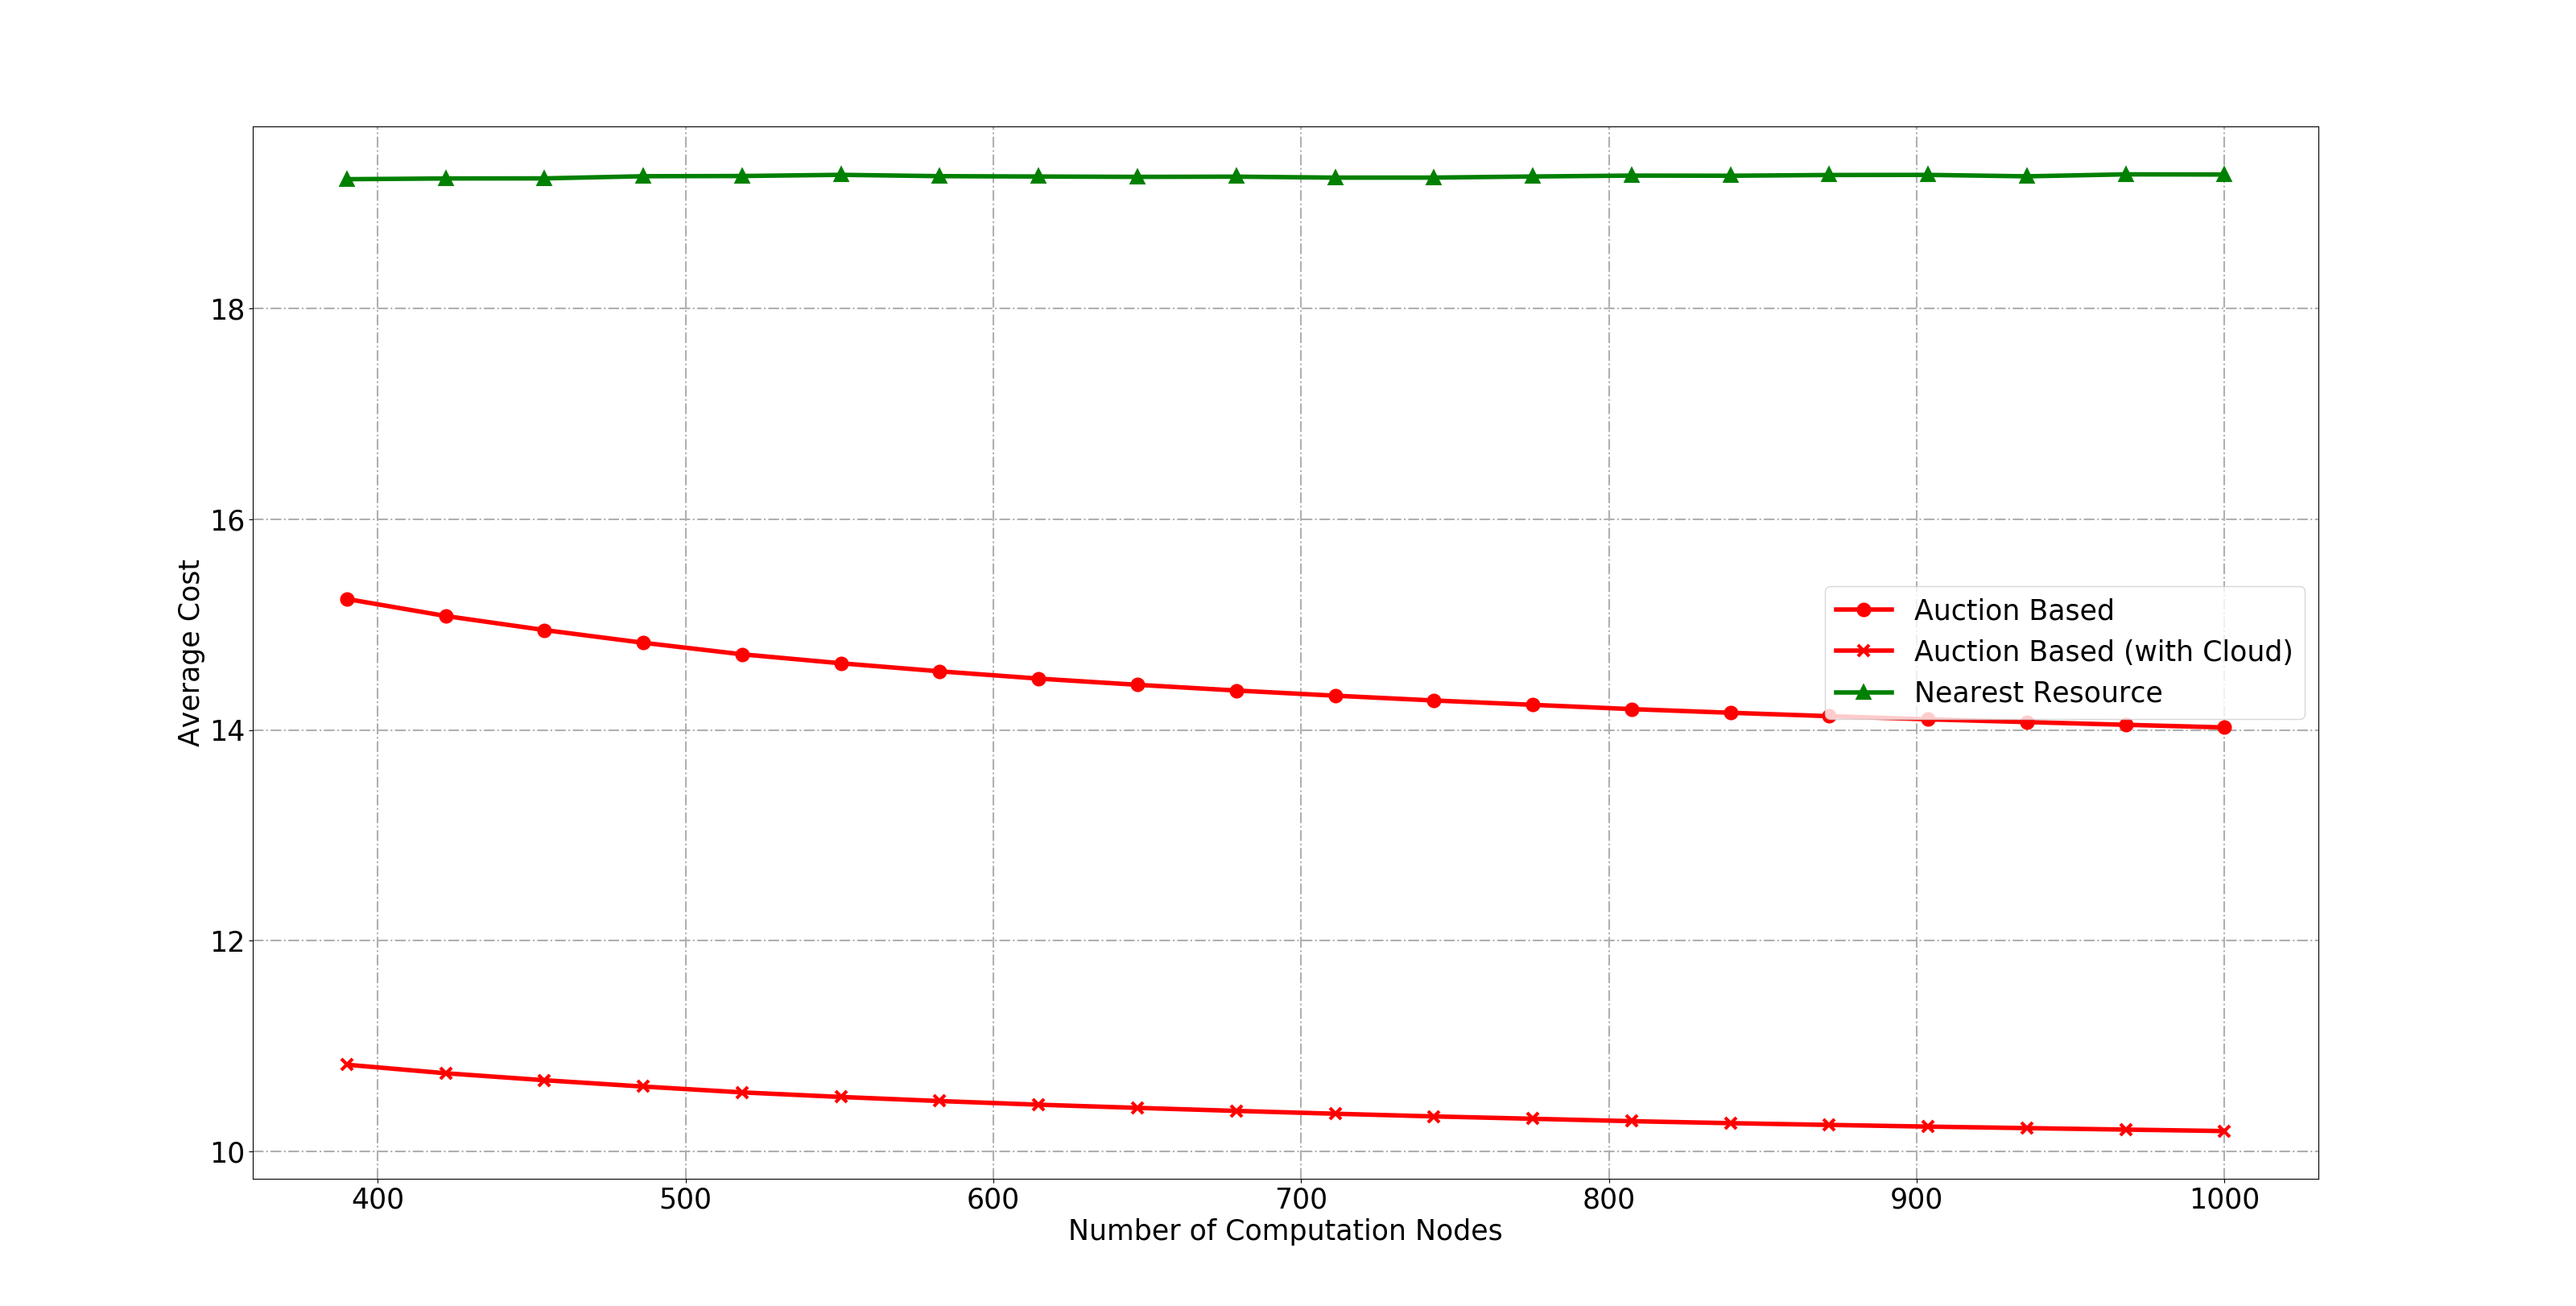
\includegraphics[width=17cm]{graphics/one_to_one/sim_1}}
      \caption{میانگین هزینه سرویس‌ها در برابر تعداد منابع پردازشی در لبه شبکه}
      \label{fig:ono_to_one:sim1}
    \end{figure}

    \cref{fig:ono_to_one:sim1} نتیجه شبیه سازی را برای سناریو‌های بیان شده نشان می‌دهد.
    برای مقایسه، نتیجه حاصل از اختصاص نزدیک‌ترین منبع پردازشی هم در شکل آورده شده است.
    در اختصاص نزدیک‌ترین منبع پردازشی، هر سرویس از نزدیک‌ترین منبع پردازشی به خود استفاده می‌کند.
    همان‌طور که از شکل مشخص است، تخصیص منابع مبتنی بر مزایده نتیجه بهتری نسبت به اختصاص نزدیک‌ترین منبع دارد.
    همان‌گونه که قبلا اشاره شد، زمانی که الگوریتم تخصیصی منابع پردازشی مبتنی بر حراج پایان می‌یابد، $U$ حداکثر به اندازه‌ی $N\epsilon$ با مقدار بیشینه فاصله دارد.
    بنابراین در هنگامی که الگوریتم پایان می‌یابد میانگین هزینه سرویس‌ها حداکثر به اندازه $\epsilon$ با مقدار کمینه فاصله دارد.
    در نتیجه برای مقادیر کوچک $\epsilon$ میانگین هزینه‌ها مقداری نزدیک به بهینه را خواهد داشت.

    از \cref{fig:ono_to_one:sim1} می‌توان استنباط کرد که با افزایش تعداد منابع پردازشی، میانگین هزینه‌ی سرویس‌ها کاهش پیدا می‌کند.
    افزایش تعداد منابع پردازشی باعث افزایش احتمال یافتن منبع پردازشی بهتر برای هر سرویس می‌شود.
    پس کاهش هزینه، نتیجه‌ای قابل قبول برای افزایش تعداد منابع پردازشی می‌باشد.
    نکته‌ی دیگری که می‌توان از این شکل برداشت کرد این است که با افزایش تعداد گره‌های پردازشی، فاصله‌ی بین میانگین هزینه سرویس‌ها در سناریو‌ای که فراهم کننده منابع پردازشی ابری حضور دارد با سناریو‌ای که فراهم کننده منابع پردازشی ابری حضور ندارد کم می‌شود.
    دلیلی که می‌توان برای آن تصور کرد این است که با افزایش تعداد گره‌های پردازشی لبه شبکه احتمال اینکه سرویس‌ها، گره‌های پردازشی لبه شبکه را انتخاب کنند بیشتر می‌شود در نتیجه سرویس‌های کمتری از منابع پردازشی ابری استفاده خواهند کرد.
    با کاهش تعداد سرویس‌هایی که از منابع پردازشی ابری استفاده می‌کنند، اثر آن‌ها در میانگین هزینه سرویس‌ها کاهش پیدا می‌کند.
    در نتیجه تفاوت دو سناریو کاهش پیدا می‌کند.

    \begin{figure}
      \centerline{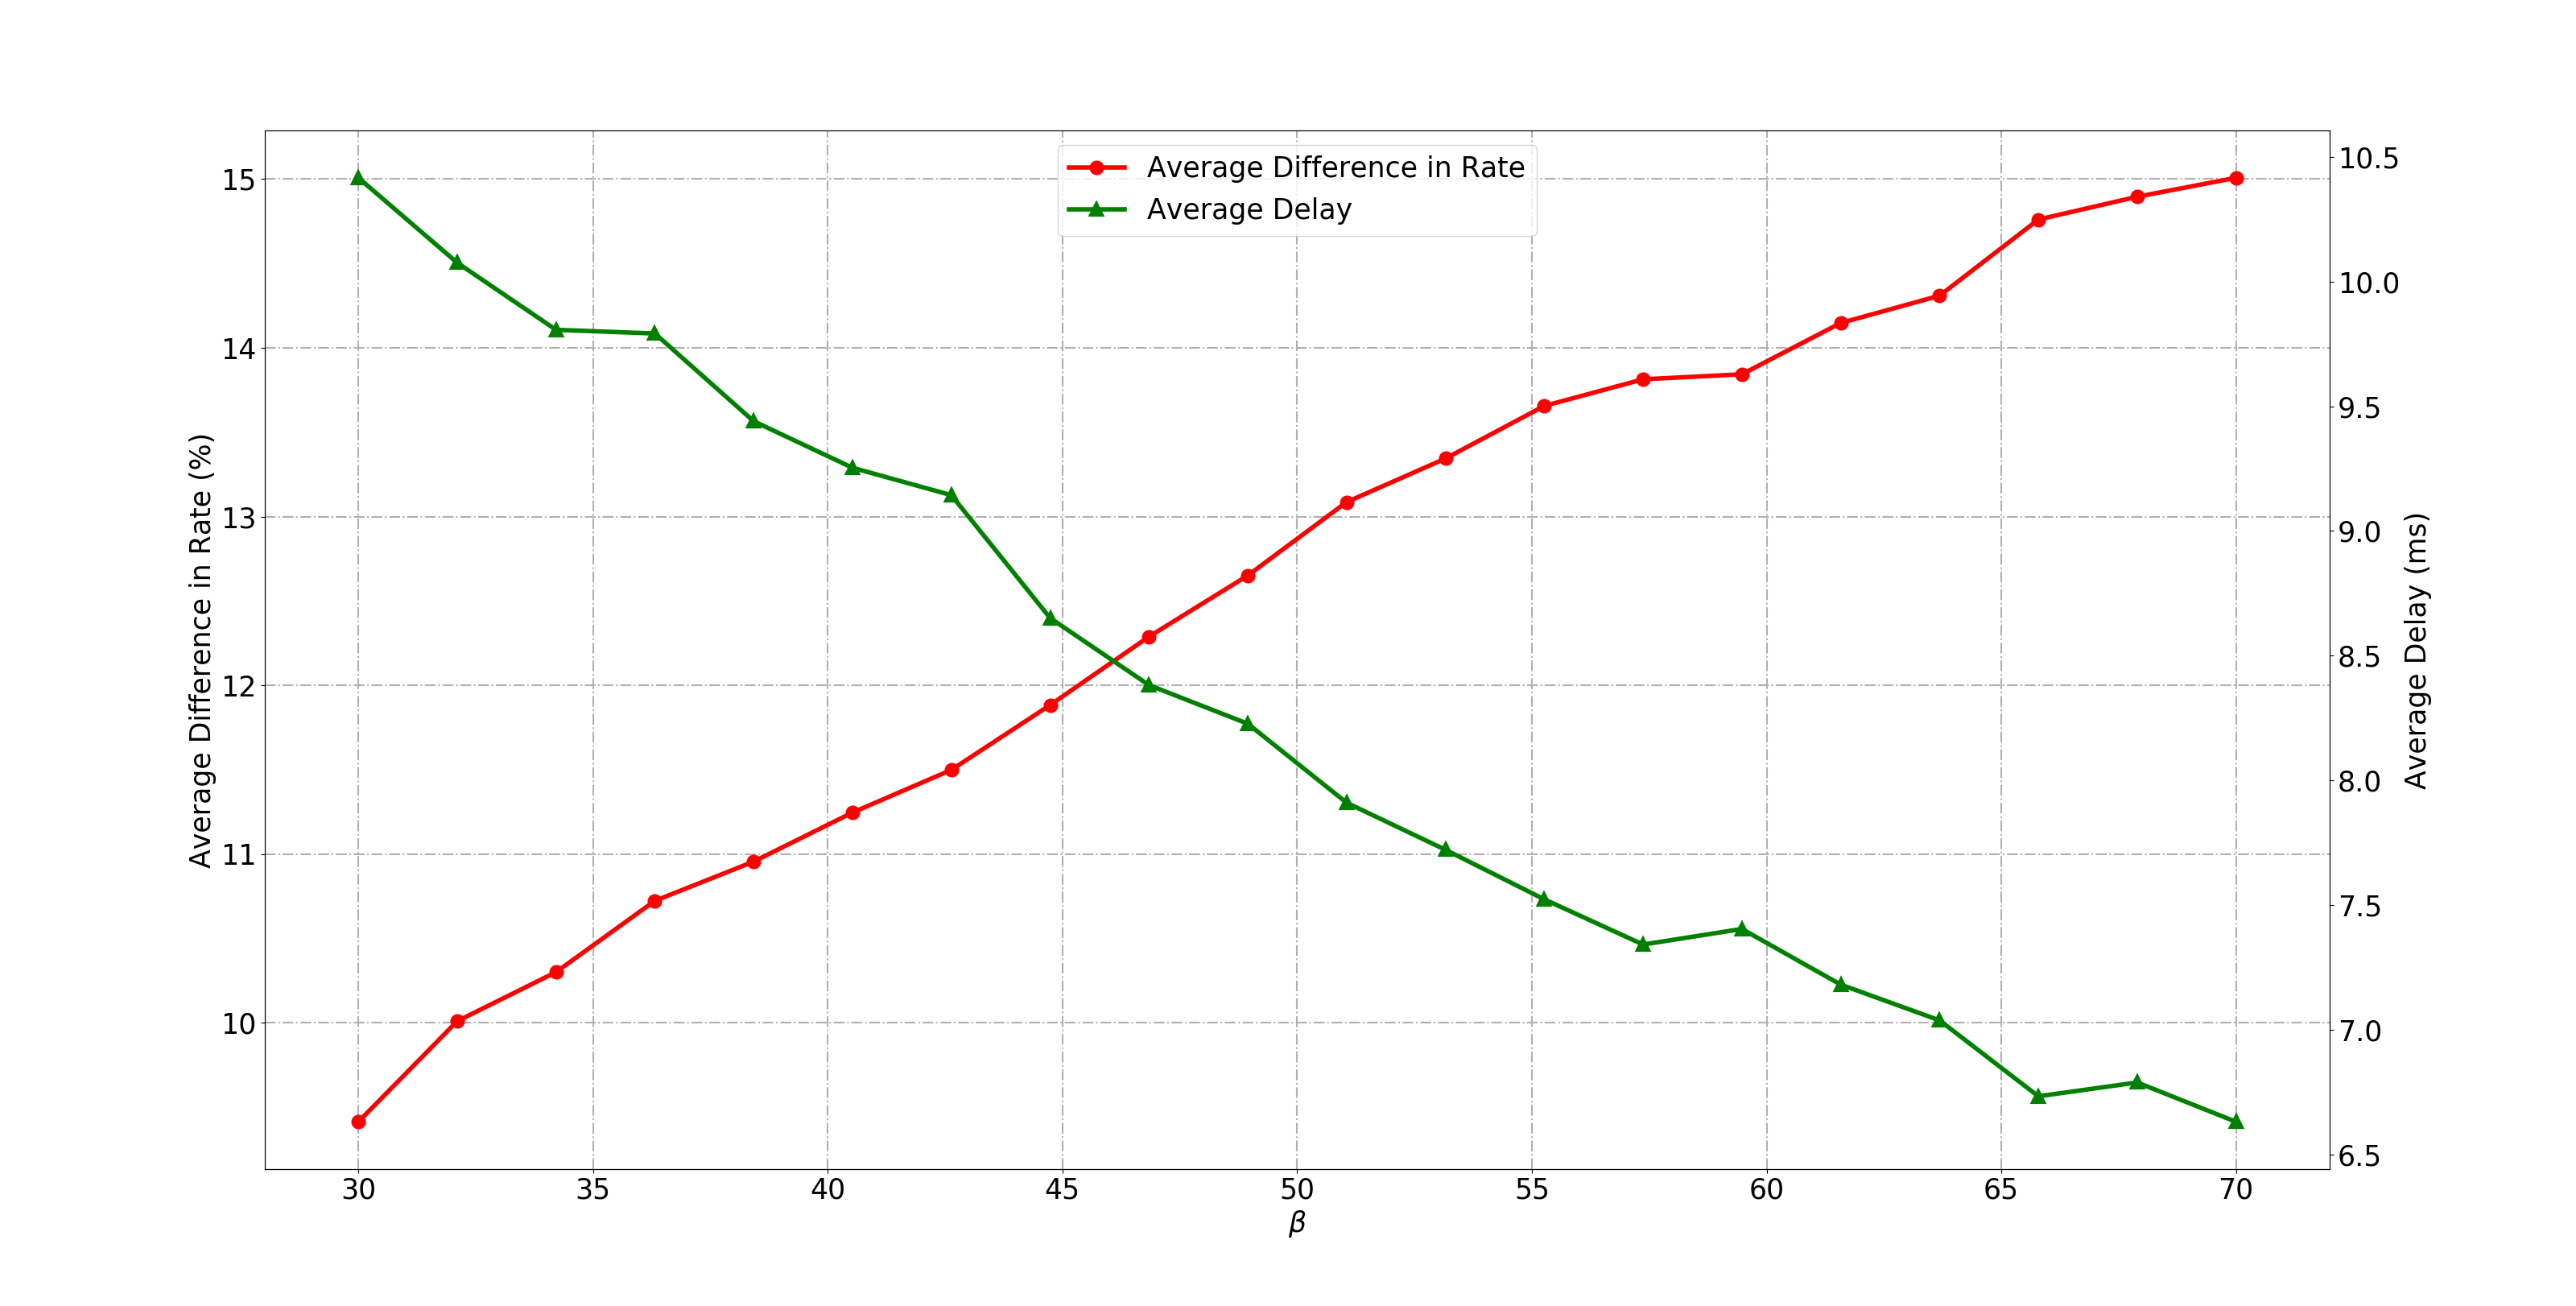
\includegraphics[width=17cm]{graphics/one_to_one/sim_2}}
      \caption{تاثیر $\beta$ بر تاخیر و اختلاف نرخ بهینه با نرخ مطلوب برای یک سرویس}
      \label{fig:ono_to_one:sim2}
    \end{figure}

    \cref{fig:ono_to_one:sim2} اثر $\beta$ روی میانگین تاخیر و میانگین اختلاف بین نرخ مطلوب و نرخ بهینه را برای یک سرویس نشان می‌دهد.
    در این شکل پارامتر‌های یاد شده برای $\beta \in [30, 70]$ رسم شده‌اند.
    در این‌جا فرض شده که همه پارامتر‌ها مانند قسمت قبل هستند و فرض شده که تأمین کننده‌ی منابع پردازشی ابری در شبکه حضور دارد.
    همان طور که قبلا بیان شد، $\beta$ بیان کننده نسبت اهمیت تاخیر به اختلاف نرخ مطلوب با نرخ بهینه است.
    به همین دلیل با افزایش $\beta$، اختلاف نرخ افرایش و تاخیر کاهش پیدا می‌کند.
    
    \begin{figure}
      \centerline{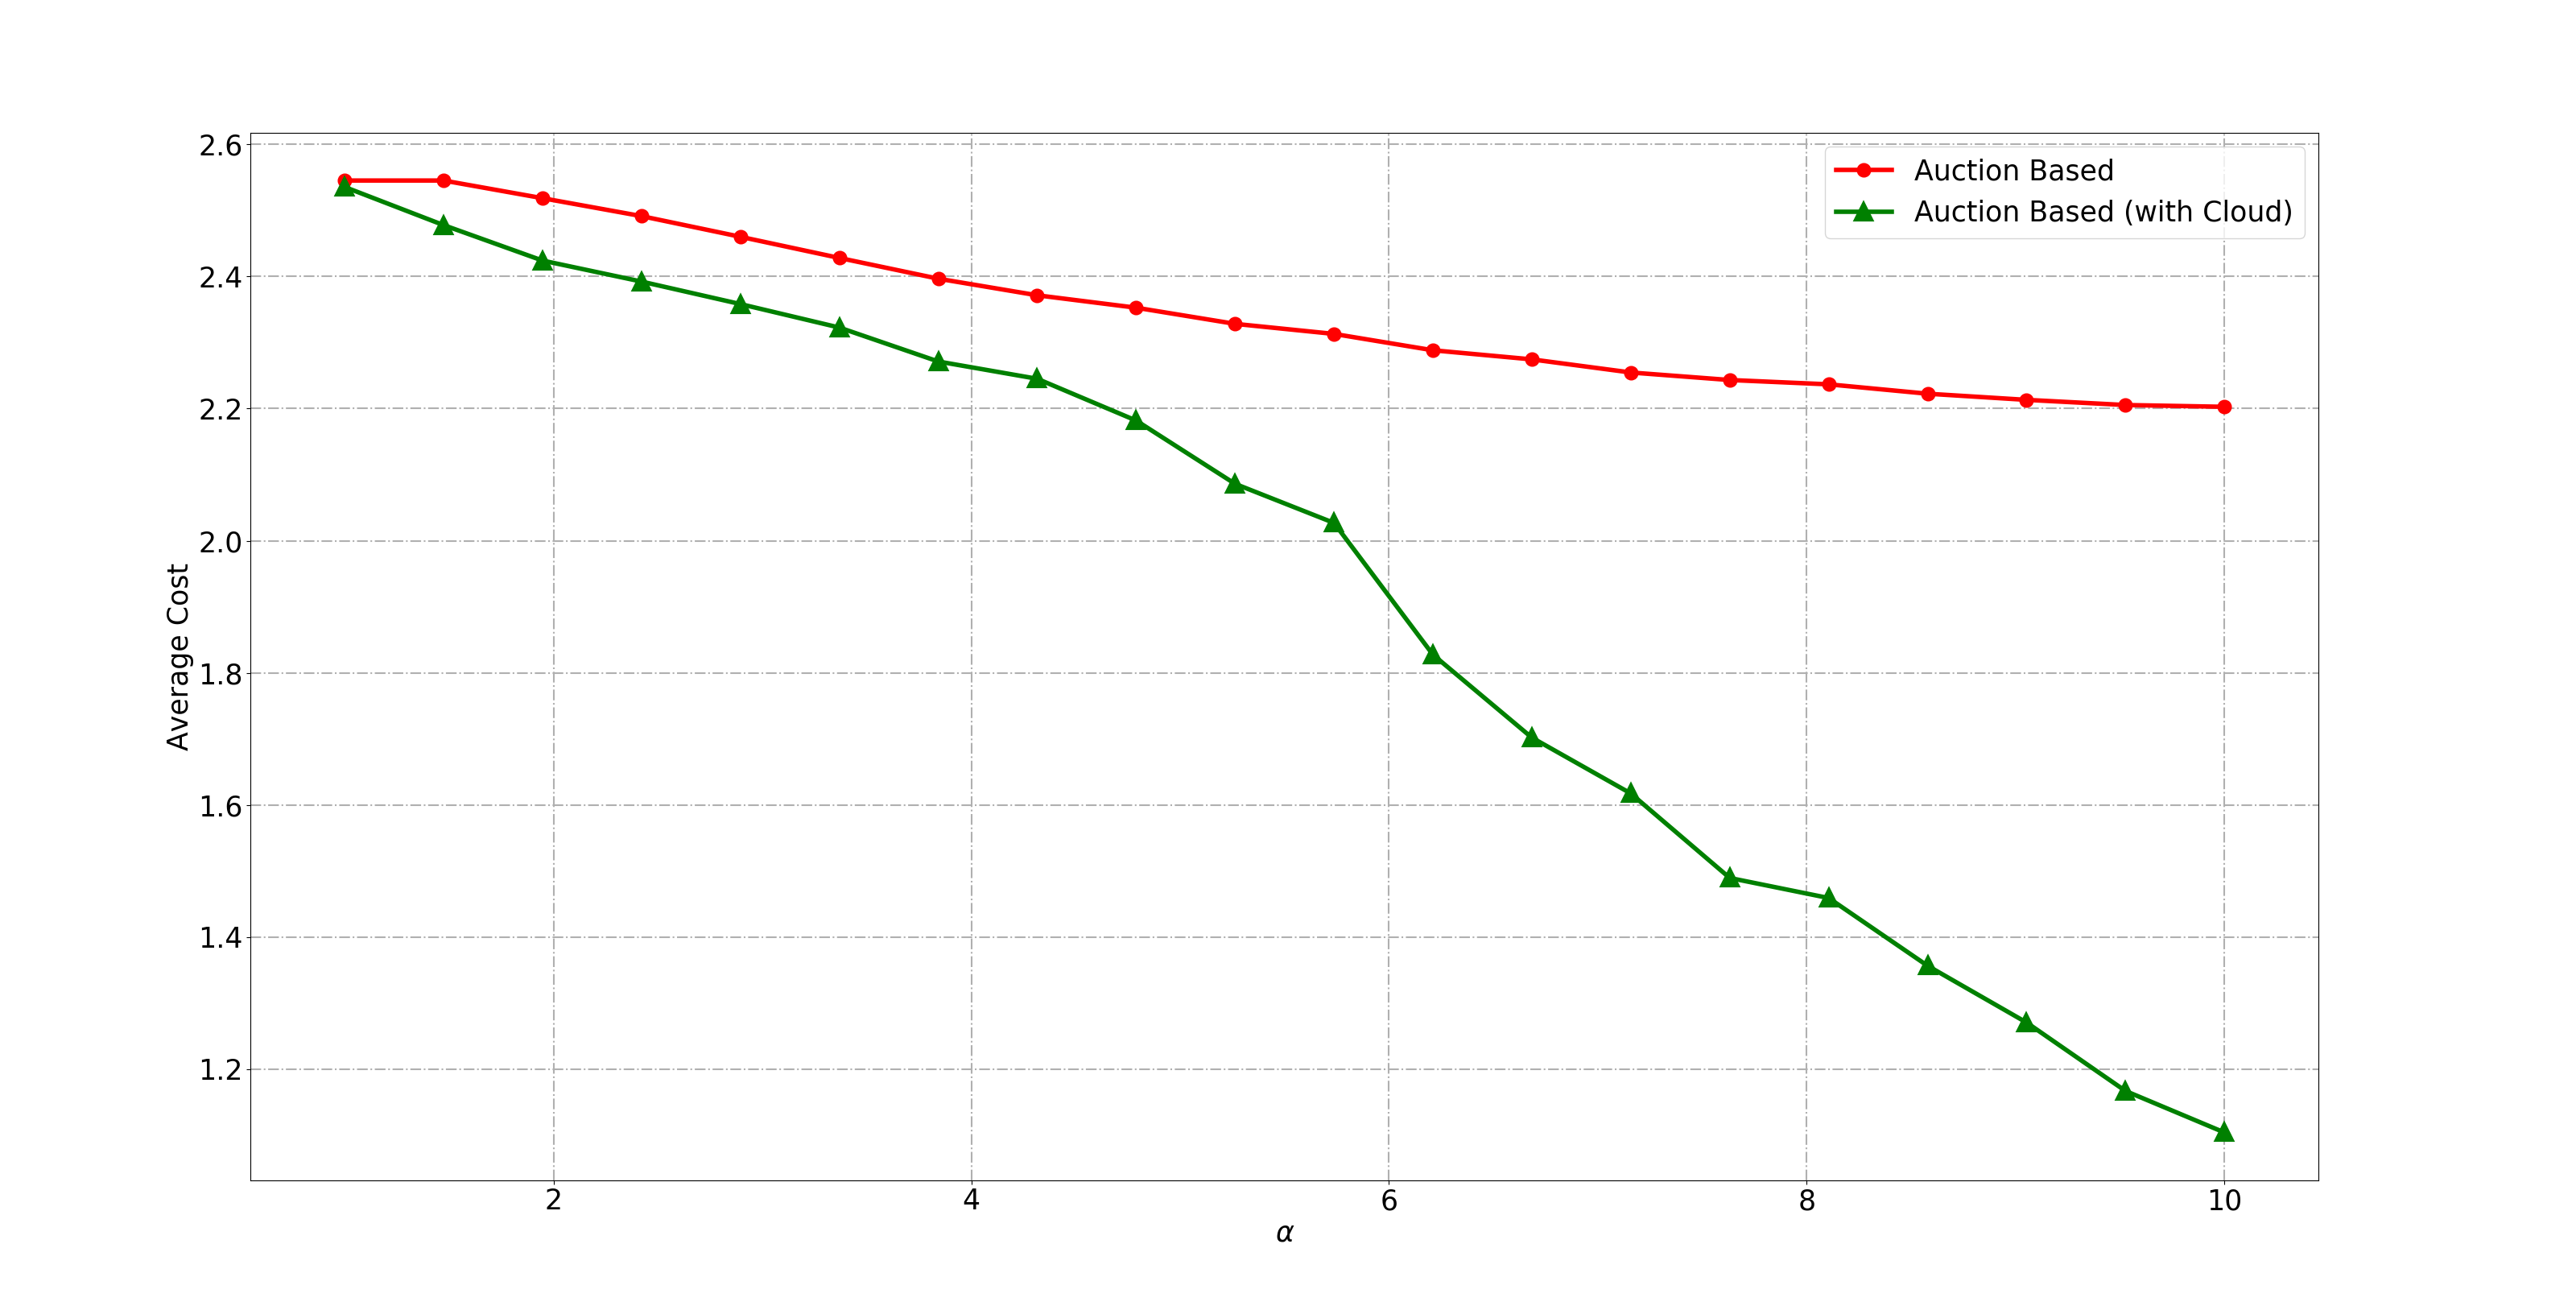
\includegraphics[width=17cm]{graphics/one_to_one/sim_3}}
      \caption{تاثیر $\alpha$ بر میانگین هزینه سرویس‌ها}
      \label{fig:ono_to_one:sim3}
    \end{figure}

    در \cref{fig:ono_to_one:sim3} تاثیر تغییر $\alpha_s$ بر روی هزینه یک سرویس‌ بررسی شده‌است.
    برای مقایسه، به جای رسم $-U_s$ برای سرویس، $-U_s/\alpha_s$ رسم شده‌است.
    واضح است که افزایش $\alpha_s$، باعث افزایش اثر تاخیر و اختلاف نرخ مطلوب و نرخ بهینه سرویس $s$ در تابع هدف بهینه سازی می‌شود.
    در نتیجه انتظار داریم با افزایش $\alpha_s$، $U_s/\alpha_s$ افزایش پیدا کند که \cref{fig:ono_to_one:sim3} این موضوع را تایید می‌کند.

    \begin{figure}
      \centerline{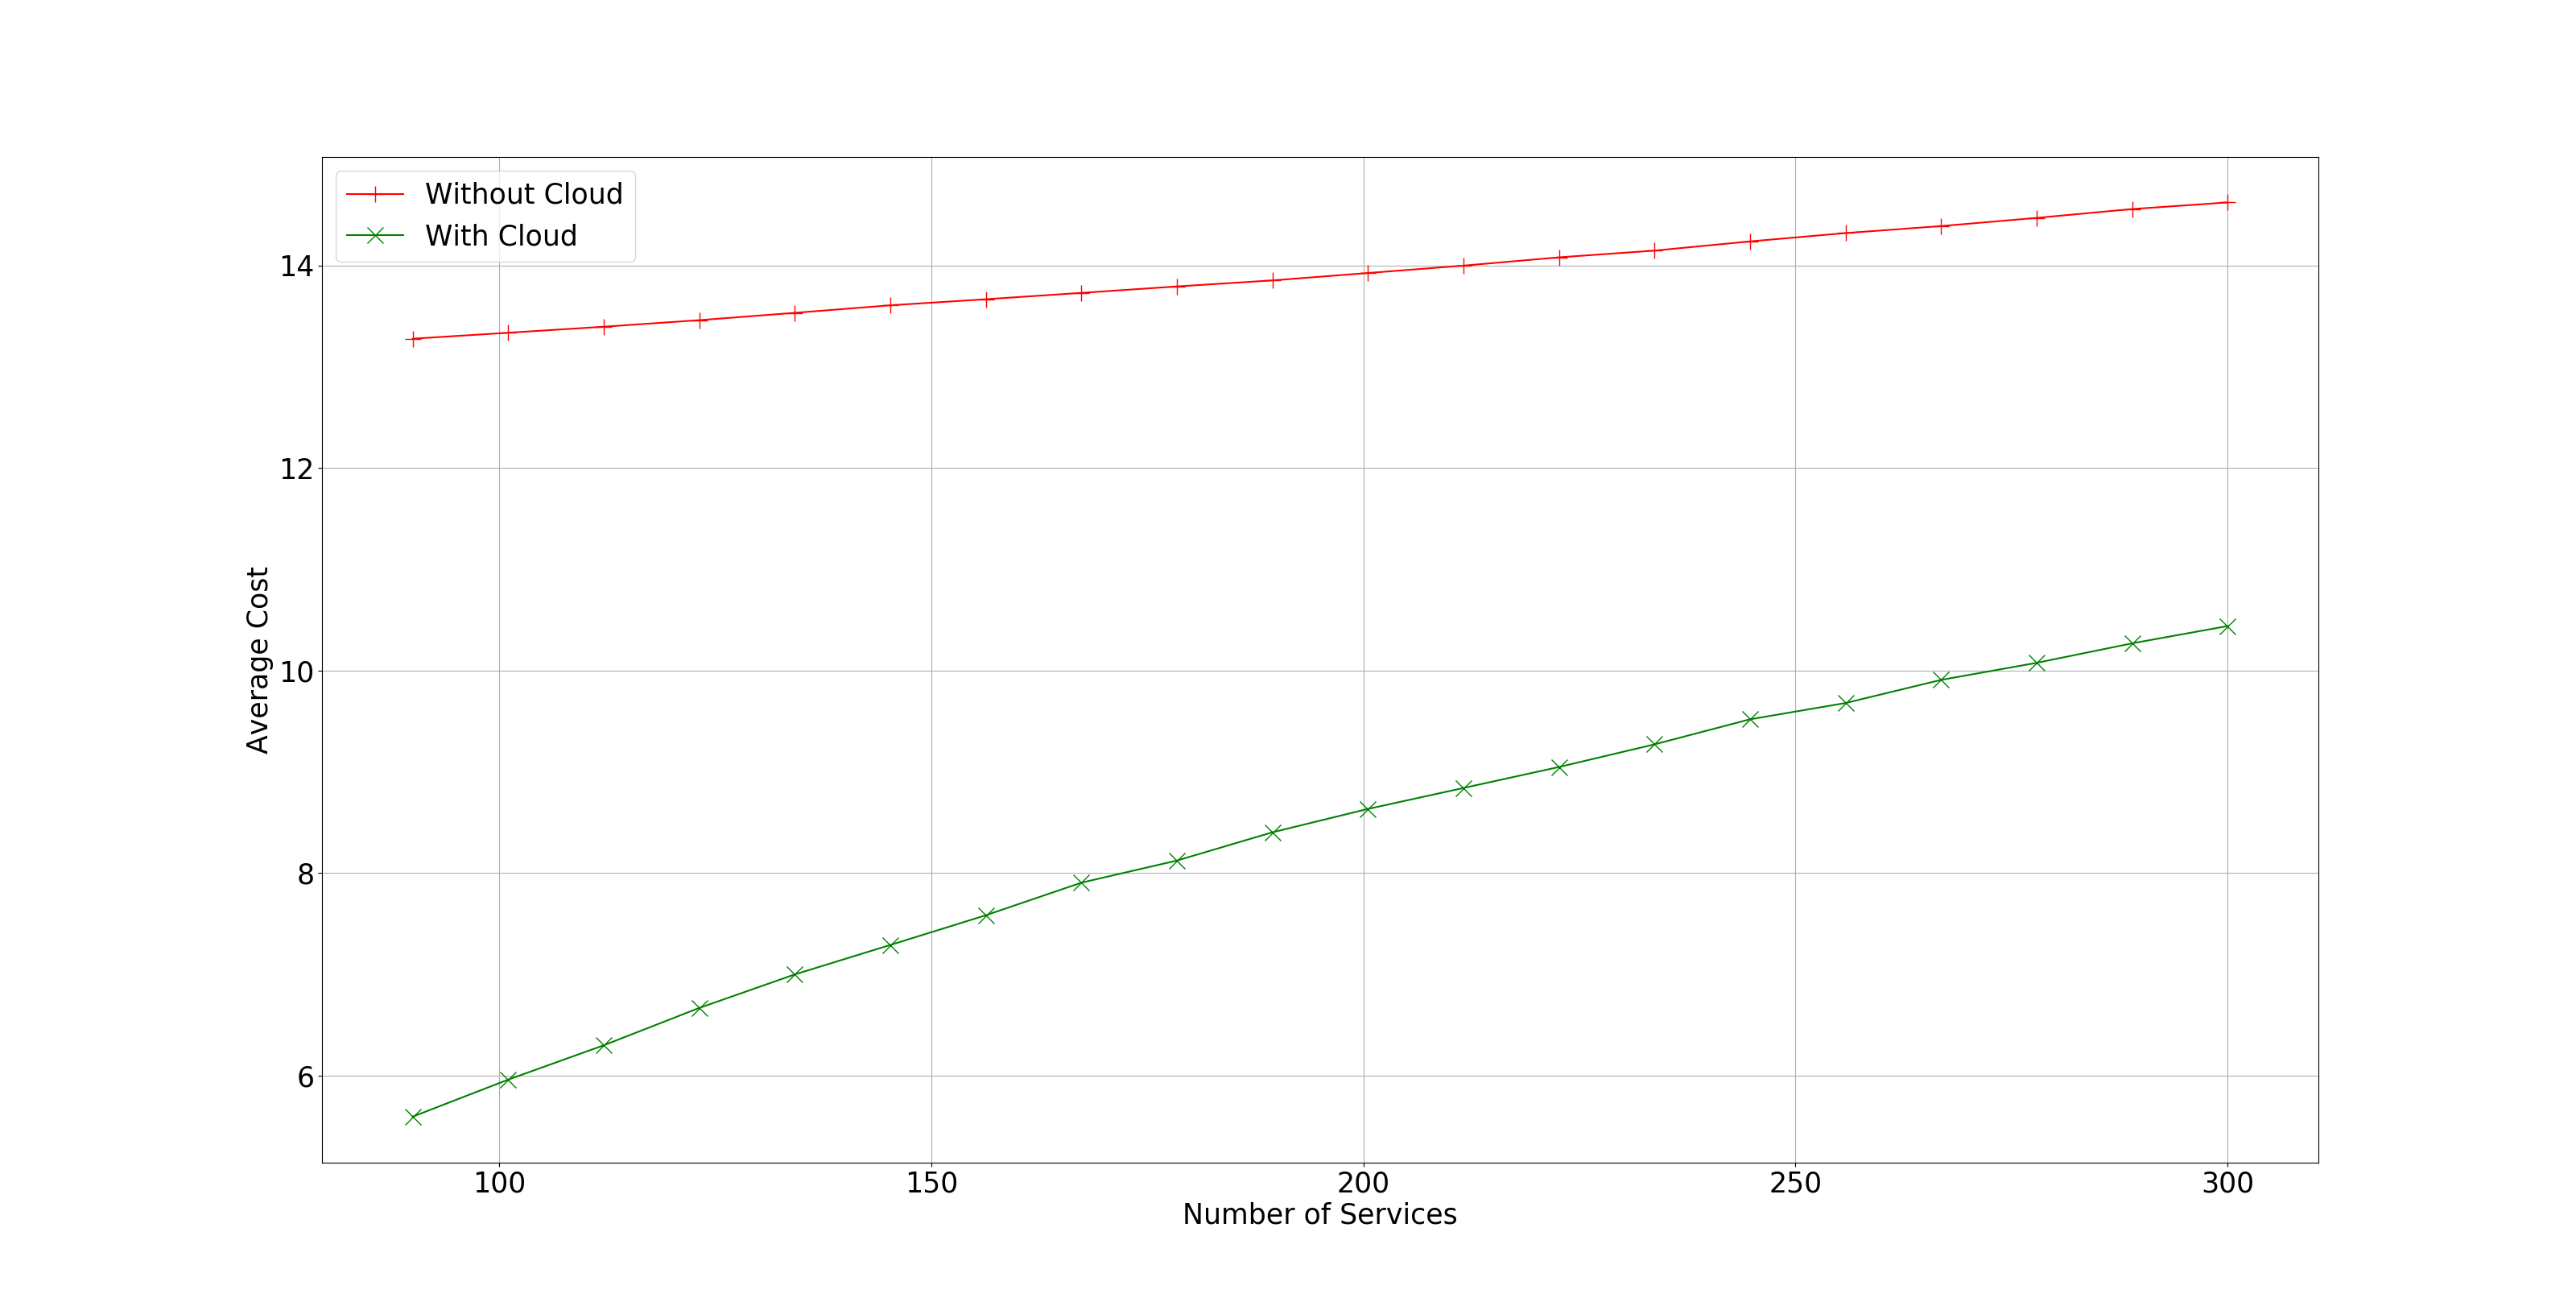
\includegraphics[width=17cm]{graphics/one_to_one/sim_4}}
      \caption{تاثیر تعداد سرویس‌ها بر میانگین هزینه سرویس‌ها}
      \label{fig:ono_to_one:sim4}
    \end{figure}

    \cref{fig:ono_to_one:sim4} تاثیر تعداد سرویس‌ها بر روی میانگین هزینه سرویس‌ها را وقتی تعداد منابع پردازشی ثابت است،‌نشان می‌دهد.
    واضح است که با ثابت بودن منابع پردازشی، افزایش تعداد سرویس‌ها باعث افزایش رقابت برای یافتن بهترین منبع پردازشی می‌شود.
    در نتیجه احتمال دریافت بهترین منبع توسط منابع پردازشی کم‌ می‌شود.

    \begin{figure}[H]
      \centerline{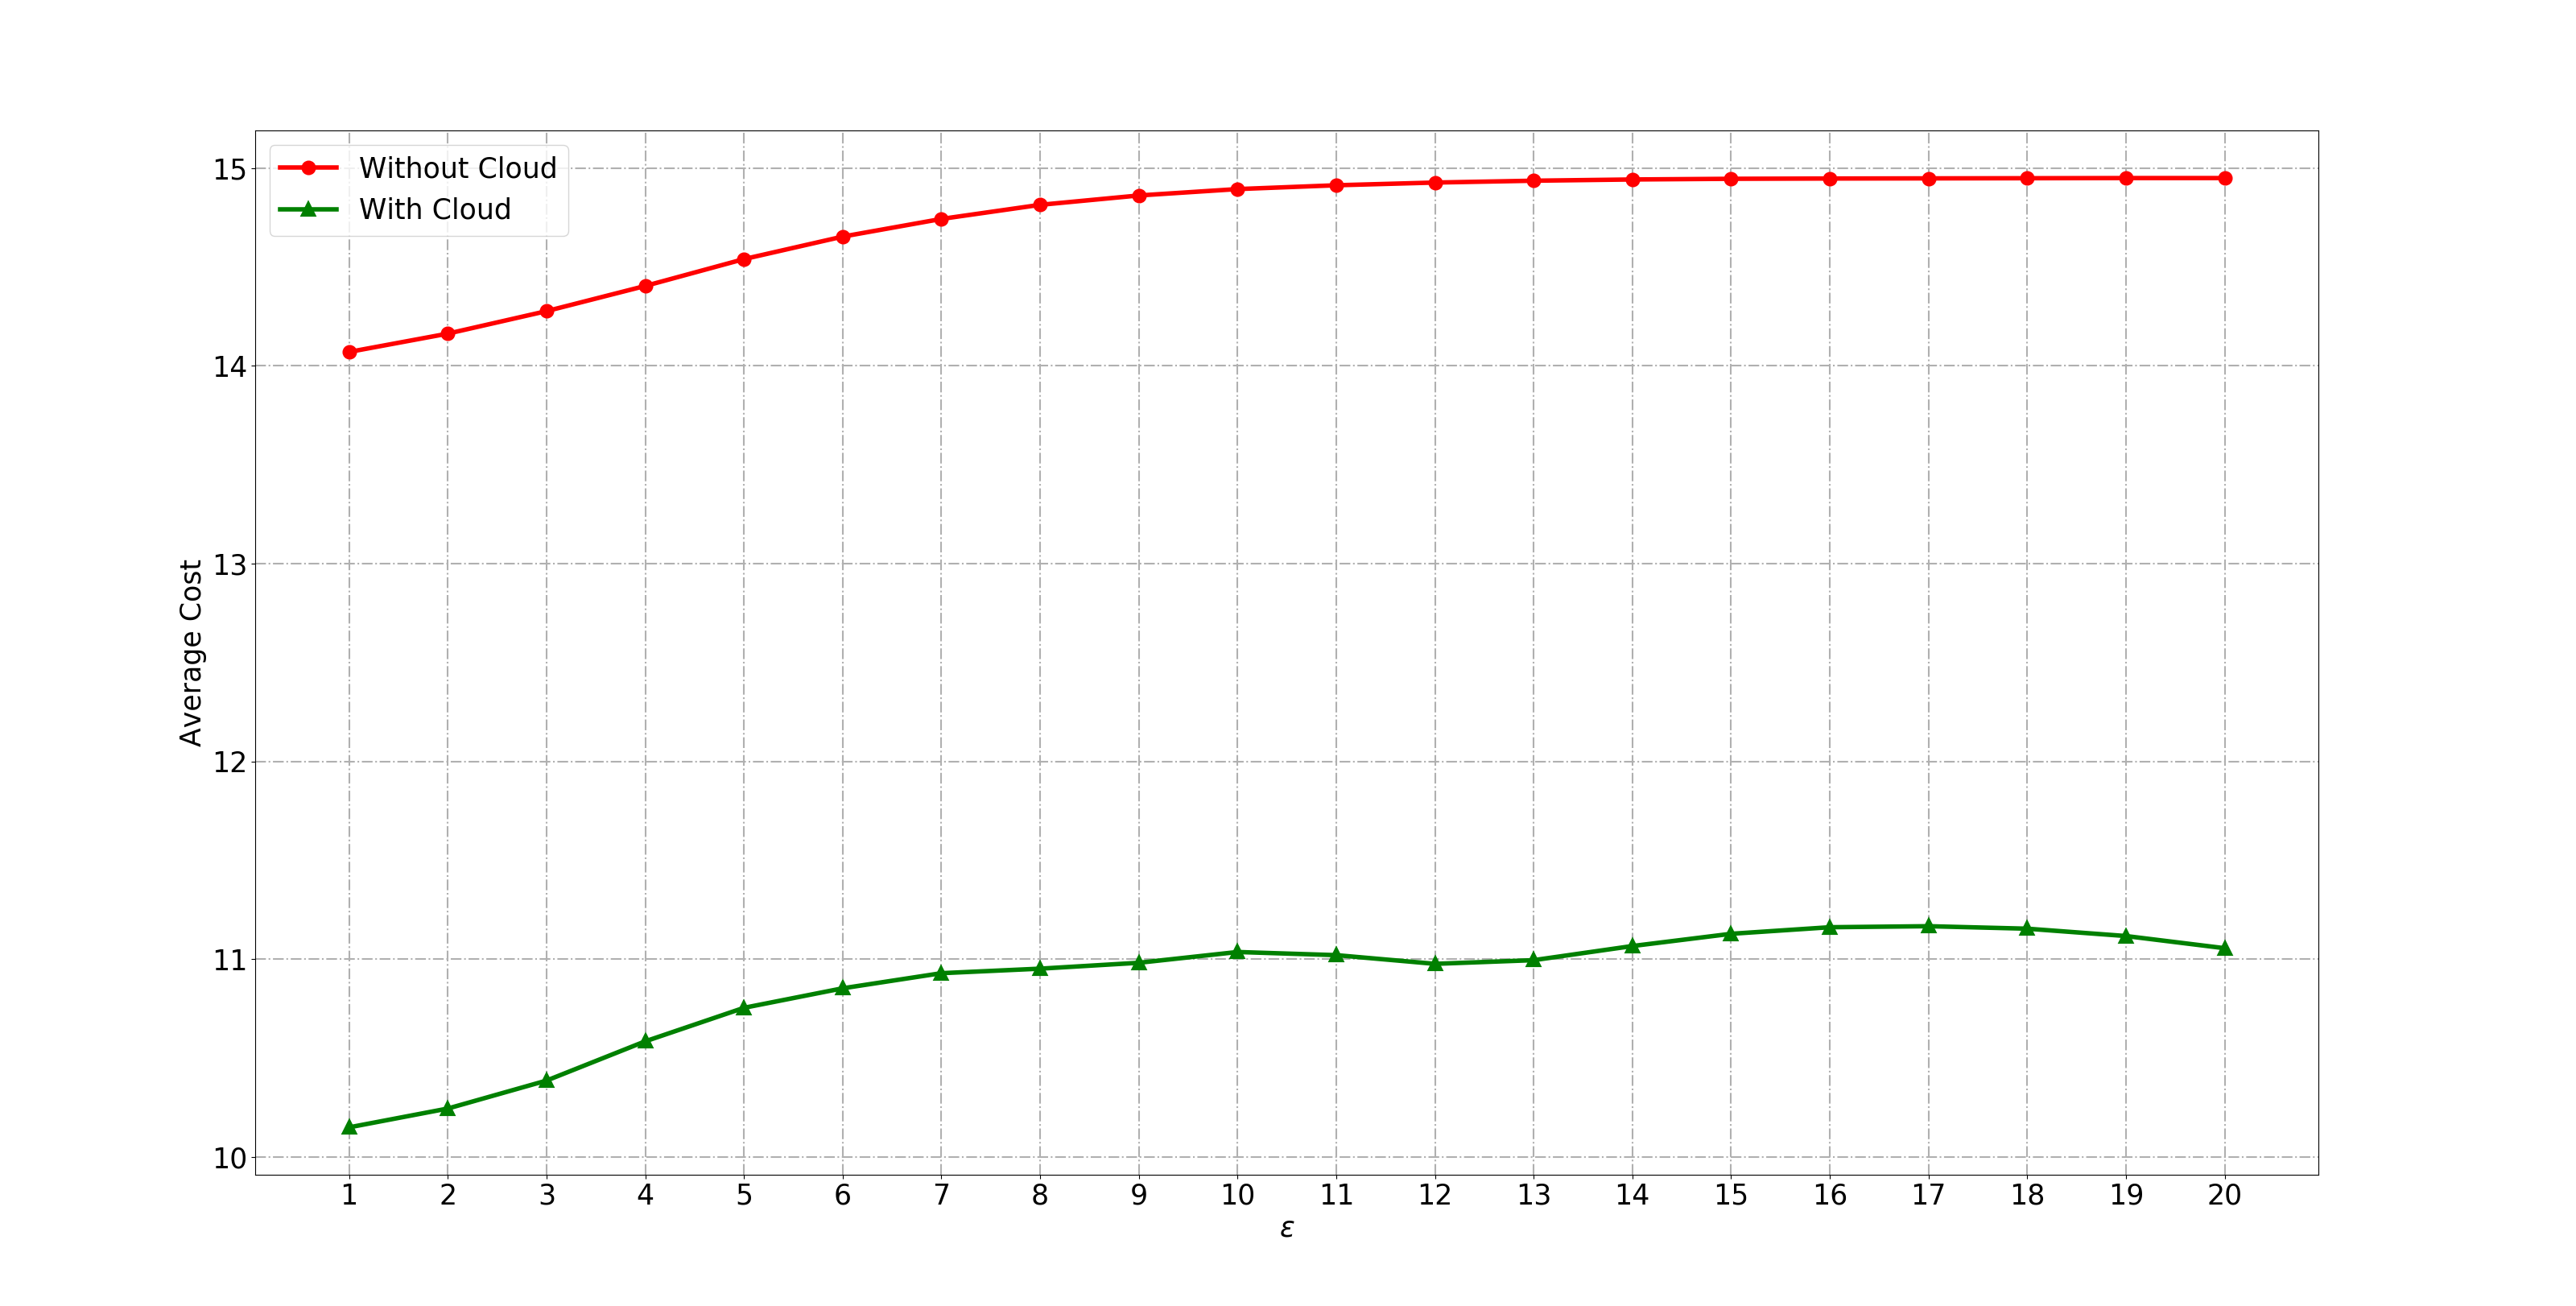
\includegraphics[width=17cm]{graphics/one_to_one/sim_5}}
      \caption{تاثیر $\epsilon$ بر میانگین هزینه‌ی همه‌ی سرویس‌ها}
      \label{fig:ono_to_one:sim5}
    \end{figure}

    در انتها در \cref{fig:ono_to_one:sim5} تاثیر $\epsilon$ بر نتیجه تخصیص منابع مشاهده می‌شود.
    مطابق مطالب بیان شده درباره‌ی روش تخصیص منابع مبتنی بر حراج با افزایش $\epsilon$ حد اکثر فاصله‌ی تخصیص منابع با مقدار بهینه بیشتر می‌شود و \cref{fig:ono_to_one:sim5} این موضوع را تأیید می‌کند.

  \section{جمع‌بندی و نتیجه‌گیری}
    در این فصل صورت مسئله تخصیص منابع پردازشی به صورت یک به یک برای سرویس‌های اینترنت اشیاء در یک شبکه بررسی شد.
    سپس الگوریتمی مبتنی بر مزایده معرفی  شد که مسئله فوق را در زمان قابل قبول حل می‌کند.
    پس از آن همگرایی، پیچیدگی و بهینگی الگوریتم مبتنی بر مزایده بررسی شد که نشان می‌داد این الگوریتم، الگوریتم مناسبی برای استفاده در تخصیص منابع در شبکه اینترنت اشیاء است.
    در انتها نتیجه شبیه‌سازی‌ برای بررسی کارایی تخصیص منابع پردازشی توسط مزایده ارائه شد.

\chapter{تخصیص منابع پردازشی در شبکه اینترنت اشیاء به صورت چند به چند}\label{Chap:many_to_many_allocation}
  \thispagestyle{empty}
  \section{مقدمه}
    در \cref{chap:one_to_one_allocation} تخصیص منابع پردازشی در شبکه اینترنت اشیاء به صورت یک به یک را بررسی کردیم.
    روش معرفی شده در \cref{chap:one_to_one_allocation} برای شرایطی مناسب است که ظرفیت پردازشی مورد نیاز سرویس‌ها با ظرفیت پردازش ارائه شده توسط منابع پردازشی در یک مرتبه باشند.
    واضح است که این شرط در شبکه‌‌های واقعی اینترنت اشیاء قابل قبول نیست.
    علاوه بر این در \cref{chap:one_to_one_allocation} فرض بر این بود که منابع پردازشی ابری با دارای ظرفیت‌های از پیش تعیین شده‌ای هستند که این فرض هم ممکن است در بعضی حالت‌ها قابل قبول نباشد.
    برای حل این مشکلات،‌ در این فصل به بررسی تخصیص منابع پردازشی در شبکه اینترنت اشیاء به صورت چند به چند می‌پردازیم.
    در این نوع از تخصیص منابع، سرویس ها می‌توانند از چند منبع پردازشی برای پردازش داده‌های سنسور‌های خود استفاده کنند و منابع پردازشی هم می‌توانند به چند سرویس اختصاص پیدا کنند.

    در ادامه ابتدا مدل سیستم را توضح می‌دهیم و تفاوت آن را با تخصیص منابع یک به یک مشخص می‌کنیم.
    سپس مانند فصل قبل مسأله تخصیص منابع را به صورت یک مسأله بهینه سازی فرمول بندی می‌کنیم.
    در ادامه یک الگوریتم برای حل این مسأله بهینه سازی معرفی کرده و در انتها نتایج شبیه‌سازی الگوریتم ارائه شده را بررسی می‌کنیم.
  \section{مدل سیستم}
    \begin{figure}[]
      \centerline{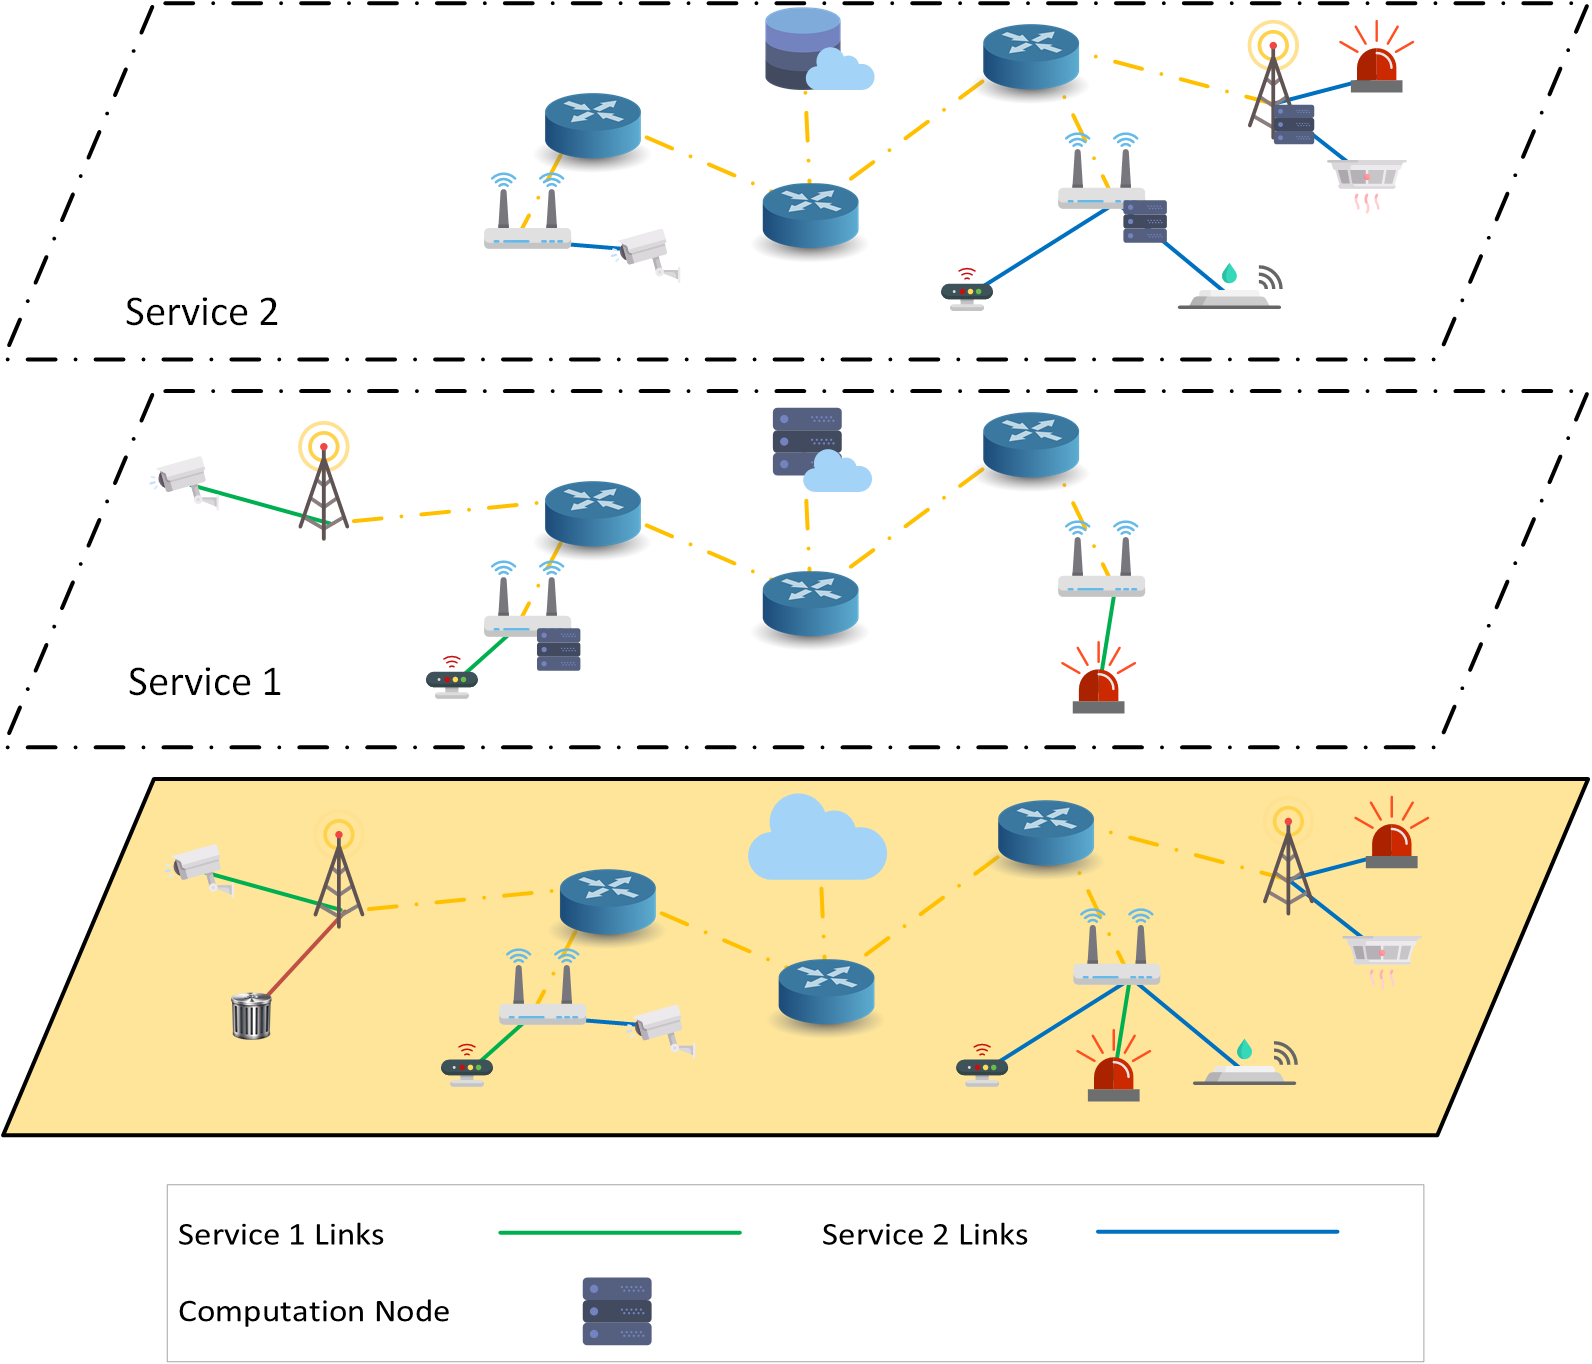
\includegraphics[width=15cm]{graphics/many_to_many/system_model}}
      \caption{مدل سیستم}
      \label{fig:many_to_many:system_model}
    \end{figure}
    در این بخش مدل سیستم برای تخصیص منابع پردازشی در شبکه اینترنت اشیاء به صورت چند به چند را توضیح می‌دهیم.
    \cref{fig:many_to_many:system_model} مدل سیستم این فصل را نشان می‌دهد که دارای دو سرویس است.
    سرویس اول از یک منبع پردازشی لبه شبکه به همراه منابع پردازشی ابری و سرویس دوم از دو منبع پردازشی لبه شبکه برای پردازش استفاده می‌کند و یکی از مقاصد نتایج پردازش‌ها ابر است.

    \cref{tbl:many_to_many:notation} به صورت خلاصه پرامتر‌های استفاده شده در این فصل را معرفی می‌کند.
    از تکرار معرفی پارامتر‌هایی که در  \cref{chap:one_to_one_allocation} استفاده شده‌اند، صرف نظر شده‌است.
    \begin{table}[h]
      \caption{نماد‌های استفاده شده در این فصل}
      \begin{tabularx}{\textwidth}{|c|C|} \hline
        نشانه             & توضیح                                                                  \\ \hline
        $I_s$             & مجموعه منابع پردازشی که سرویس $s$ از آن‌ها استفاده می‌کند                \\ \hline
        $I_i$             & مجموعه سرویس‌هایی که منبع پردازشی $i$ به آن‌ها اختصاص پیدا کرده‌است       \\ \hline
        $C_s$             & مجموعه منابع پردازشی که سرویس $s$ می‌تواند از آن‌ها استفاده می‌کند        \\ \hline
        $S_i$             & مجموعه سرویس‌هایی که منبع پردازشی $i$ می‌تواند به آن‌ها اختصاص پیدا کند   \\ \hline
        $Q_s$             & حداکثر تعداد منابع پردازشی که سرویس $s$ مجاز به استفاده از آن‌ها است    \\ \hline
        $Q_i$             & حداکثر تعداد سرویس‌هایی که منبع پردازشی $i$ می‌تواند به آن‌ها اختصاص پیدا کند  \\ \hline
        $d_{i,s}$         & تأخیر منبع پردازشی $i$ برای سرویس $s$                                       \\ \hline
        $d_s^\text{max}$  & بیش‌ترین تاخیر سرویس $s$ بین منابع پردازشی اکه از آن‌ها استفاده می‌کند         \\ \hline
        $r_{i,s}$         & نرخی که سرویس $s$ برای پردازش به منبع پردازشی $i$ می‌فرستد                   \\ \hline
        $u_{i,s}$         & بخشی از ضرفیت پردازشی منبع پردازشی $i$ که توسط سرویس $s$ استفاده می‌شود      \\ \hline
      \end{tabularx}
      \label{tbl:many_to_many:notation}
    \end{table}
    مانند فصل قبل تابع هدف بهینه سازی از دو قسمت تشکیل می‌شود که قسمت اول تابع نرخ انتخابی سرویس‌ها و قسمت دوم مربوط به تاخیر‌ها است
    \begin{equation}
      U_s = \alpha_s \left ( \omega_s f_r(r_s, R_s) + (1-\omega_s) f_d(d_s^\text{max}) \right ) .
    \end{equation}
    در این رابطه $r_s$ مجموع نرخی است که توسط منابع پردازشی برای سرویس $s$ پردازش می‌شود.
    در نتیجه رابطه زیر برای $r_s$ برقرار است
    \begin{equation}
      r_s = \sum_{i \in C_s}^M r_{i,s} .
    \end{equation}
    چون در این فصل فرض بر این است که هر سرویس می‌تواند از چند منبع پردازشی استفاده کند، بیشترین تاخیر منابع پردازشی مورد استفاده سرویس‌ها را به عنوان تاخیر آن سرویس در نظر می‌گیریم.
    اگر فرض کنیم $d_{i,s}$ تاخیر پردازش سرویس $s$ در منبع پردازشی $i$ و $d_s^\text{max}$ بیشترین تاخیر سرویس $s$ باشد، قید زیر برای همه منابع پردازشی انتخاب شده توسط سرویس $s$ باید برقرار باشد
    \begin{equation}\label{eqn:max_delay}
      d_{i,s} < d_s^{max}; \forall s \in S, i \in C_s, \delta_{i,s} = 1.
      این تاخیر مانند فصل قبل برای هر منبع پردازشی از دو قسمت تشکیل شده‌است.
    \end{equation}
    قسمت اول آن مربوط به تاخیر شبکه است که برابر است با زمانی که طول می‌کشد تا نمونه‌ها به منبع پردازشی برسند به علاوه زمانی که طول می‌کشد نتیجه به مقصد برسد.
    قسمت دوم تاخیر پردازش نمونه‌ها در منابع پردازشی است.
    این تاخیر برابر زمانی است که طول می‌کشد تا نمونه‌ها پس از رسیدن به منابع پردازشی، پردازششان پایان یابد.
    همانند فصل قبل برای محاسبه تاخیر پردازشی از تئوری صف استفاده می‌کنیم.
    به دلیل این‌که در این فصل فرض بر این است که منابع پردازشی بین چند سرویس ممکن است تقسیم شوند، از مدل $M/M/1$ استفاده می کنیم.
    در مدل $M/M/1$ میانگین تاخیر $\omega$ از رابطه زیر بدست می‌آید\cite{basic_queueing_sztrik}
    \begin{equation}
      \omega = \frac{1}{\mu-\lambda}.
    \end{equation}
    مانند فصل قبل، ظرفیت پردازشی منبع پردازیش $i$ را با $\varphi_i = \phi_i \nu_i$ است.
    در این فصل متغیر $u_{i,s}$ تعیین می‌کند که چه مقدار از ظریفیت پردازشی منبع پردازشی $i$ تخصیص پیدا می‌کند.
    واضح است که سرویس‌ها نمی‌توانند بیش‌تر از ظرفیت منابع پردازشی از آن‌ها استفاده کنند.
    در نتیجه رابطه زیر برای مقادیر ظرفیت‌های پردازشی تخصیص یافته به سرویس‌ها برای همه منابع پردازشی باید برقرار باشد:
    \begin{equation}
      \sum_{s \in S_i} u_{i,s} \le 1, \forall i \in C.
    \end{equation}
    مانند \cref{chap:one_to_one_allocation} نرخ سرویس برای سرویس $s$ در منبع پردازشی $i$ از رابطه زیر بدست خواهد آمد
    \begin{equation}
      \mu_{i,s} = \frac{\varphi_i}{F_s} u_{i,s} = \zeta_{i,s} u_{i,s}, \forall s \in S, i \in C_s.s
    \end{equation}
    با این تفاسیر رابطه‌ی زیر را برای تاخیر پردازشی سرویس $s$ در منبع پردازشی $i$ وقتی از آن منبع پردازشی استفاده می‌کند می‌توان نوشت
    \begin{equation}
      d_{i,s}^\text{CPU} = \frac{1}{\zeta_{i,s} u_{i,s} - r_s}.
    \end{equation}
    درنتیجه رابطه زیر برای تاخیر سرویس $s$ در منبع پردازشی $i$ برقرار است
    \begin{equation}
      d_{i,s} = d_{i,s}^\text{net} + \frac{1}{\zeta_{i,s} u_{i,s} - r_s}.
    \end{equation}
    این رابطه به عنوان قید در یک بهینه سازی محدب قابل استفاده نیست.
    به همین دلیل سعی میی‌کنیم تغییراتی در آن ایجاد کنیم تا به یک قید محدب تبدیل شود.
    با توجه به وجود $d_{i,s}^\text{max}$ در تابع هدف بهینه سازی، شرایط بیان شده برای تابع $f_d$ در \cref{chap:one_to_one_allocation} و \cref{eqn:max_delay} جزء قید‌های مسئله است، می‌توانیم علامت = را با علامت $\le$ جایگزین کنیم
    \begin{equation}
      \frac{1}{\zeta_{i,s} u_{i,s} - r_s} \le d_{i,s} - d_{i,s}^\text{net}.
    \end{equation}
    چون لگاریتم یک تابع صعودی است، می‌توان بدون مشکلی از دو طرف نامساوی، لگاریتم گرفت و علامت تغییری نکند.
    با لگاریتم گرفتن از طرفین می‌توان قید مناسب برای استفاده در بهینه سازی محدب را بدست آورد.
    \begin{equation}\label{eqn:delay_inequality}
      - \log (\zeta_{i,s} u_{i,s} - r_s) - \log (d_{i,s} - d_{i,s}^\text{net}) \le 0.
    \end{equation}
    دلیل محدب بودن \cref{eqn:delay_inequality} این است که $\zeta_{i,s} u_{i,s} - r_s$ و $d_{i,s} - d_{i,s}^\text{net}$ هر دو تابع محدب هستند.
    همچنین تابع $-\log$ هم یک تابع محدب است.
    با توجه به قضیه ترکیب توابع محدب \cite{boyd2004convex}، \cref{eqn:delay_inequality} یک قید محدب است.

    با توجه به آنچه که تا این جا گفته شد،‌ می‌توان مسئله بهینه سازی را به صورت زیر نوشت
    \begin{subequations}
      \begin{align}
        \underset{r_{i,s}, u_{i,s}, \delta_{i,s}}{\text{maximize}} \qquad & \sum_{s=1}^N \alpha_s \left (\omega_s f_r(r_s, R_s) + (1-\omega_s) f_d(d_{i,s}^\text{max}) \right ) \\
        \text{\lr{subject  to}} \qquad & \nonumber \\
        & r_s = \sum_{i \in S_i} r_{i,s}, \forall s \in S \\
        & 0 \le r_{i,s}, \forall s \in S, i \in C_s \label{eqn:rate_positiveness2} \\
        & r_{i,s} \le \eta \zeta_{i,s} u_{i,s}, \forall s \in S, i \in C_s \label{eqn:rate_saturation2} \\
        & u_{i,s} \le \delta_{i,s}, \forall s \in S, i \in C_s \label{eqn:u_le_delta} \\
        & d_{i,s} \le d_{i,s}^\text{max}, \forall s \in S, i \in C_s, \delta_{i,s}=1 \\
        &- \log \left((\zeta_{i,s} u_{i,s} - r_s) (d_{i,s} - d_{i,s}^\text{net}) \right ) \le 0, \forall s \in S, i\in C_s, \delta_{i,s}=1 \\
        & \sum_{s \in S_i} u_{i,s} \le 1, \forall i \in C \label{eqn:sum_of_utiliztion} \\
        & \sum_{s \in S_i} \delta_{i,s} \le Q_i, \forall i \in C \label{eqn:computation_quota} \\
        & \sum_{i \in C_s} \delta_{i,s} \le Q_s, \forall s \in S \label{eqn:service_quota} \\
        & \delta_{i,s} \in \{0, 1\}, \forall s \in S, i \in C_s
      \end{align}
    \end{subequations}
    در این مسئله
    قید \eqref{eqn:u_le_delta} باعث می‌شود که زمانی که سرویس $s$ از منبع پردازشی $i$ استفاده نمی‌کند $u_{i,s}=0$ باشد و در صورت استفاده $u_{i,s}<1$ باشد.
    باید توجه کرد که قیدهای \cref{eqn:rate_positiveness2} و \cref{eqn:rate_saturation2} باعث می‌شوند که $u_{i,s}$ها مثبت باشند.
    قید \eqref{eqn:sum_of_utiliztion} برای این در بهینه سازی حظور دارد که میزان استفاده از منابع پردازشی نمی‌تواند بیشتر از ظرفیت آن‌ها باشد.
    قید \eqref{eqn:computation_quota} نشان دهنده‌ی حداکثر تعداد سرویس‌هایی است که یک منبع پردازشی می‌تواند به آن‌ها اختصاص پیدا کند.
    قید \eqref{eqn:service_quota} برای محدود کردن حداکثر تعداد منابع پردازشی که یک سرویس می‌تواند استفاده کند است.
    
    مانند فصل قبل، این مسئله بهینه سازی هم یک مسئله برنامه‌ریزی غیرخطی عدد صحیح مخلوط می‌باشد که پیدا کردن جواب بهینه آن ساده نیست.
    به همین دلیل در بخش بعدی یک الگوریتم برای پیدا کردن جواب زیر بهینه آن معرفی می‌کنیم.

  \section{معرفی الگوریتم زیر بهینه}
    این الگوریتم، یک الگوریتم مبتنی بر تکرار است.
    در هر تلکرار الگوریتم، برای هر سرویس، یک تغییر در منابع پردازشی اختصاص یافته به آن سرویس ایجاد می‌کنیم.
    این تغییر می‌توان حذف کردن، اضافه کردن یا جابه‌جایی منابع پردازشی آن سرویس باشد به شرطی که پس از تغییر قید‌های حداکثر تعداد سرویس‌های منابع پردازشی و حداکثر تعداد منابع پردازشی سرویس برقرار باشند.
    این کار را در هر تکرار برای همه‌ی سرویس‌ها انجام می‌دهیم.
    برای هر سرویس هم همه حالت‌های تغییر در یک منبع پردازشی را در نظر می‌گیریم.
    پس انجام این کار، تغییری که بیشترین افزایش را در تابع هدف بهینه‌سازی دارد به تخصیص منابع اعمال می‌کنیم.
    این الگوریتم تا زمانی که مقدار افزایش تابع هدف بهینه سازی بیشتر از مقدار مشخص $\epsilon$ باشد ادامه می‌یابد.
    \cref{alg:suboptimal_algorithm} به صورت خلاصه این الگوریتم را نشان می‌دهد.

    \begin{latin}
      \begin{algorithm}[t]
        \caption{Auction ‌Based Resource Assignment Algorithm}
        \label{alg:suboptimal_algorithm}
        \begin{algorithmic}[1]
          \While{$\nu > \epsilon$}
            \For {$s \in S$}
              \For {$(c_1,c_2) \in (I_s \cup \{\_\}) \times ((C_s \setminus I_s) \cup \{\_\}) $}
                \If{$s \in S_{c_2}$}
                  \State{$I_s \gets (I_s \setminus \{c_1\}) \cup \{c_2\}$}
                  \State{$I_{c_1} \gets I_{c_1} \setminus \{s\}$}
                  \State{$I_{c_2} \gets I_{c_2} \cup \{s\}$}
                  \If{$|I_s| \le Q_s|$ and $|I_{c_2}| \le Q_{c_2}|$}
                    \State{$\nu' = $ Obtimization Objective Value}
                    \If {$\nu' > \nu$}
                      \State{$\nu \gets \nu'$}
                      \State{$s^\text{new} \gets s$}
                      \State{$c_1^\text{new} \gets c_1$}
                      \State{$c_1^\text{new} \gets c_2$}
                    \EndIf
                  \EndIf
                  \State{$I_s \gets (I_s \setminus \{c_2\}) \cup \{c_1\}$}
                  \State{$I_{c_2} \gets I_{c_2} \setminus \{s\}$}
                  \State{$I_{c_1} \gets I_{c_1} \cup \{s\}$}
                \EndIf
              \EndFor
            \EndFor
            \State{$I_s^\text{new} \gets (I_s^\text{new} \setminus \{c_1^\text{new}\}) \cup \{c_2^\text{new}\}$}
            \State{$I_{c_1}^\text{new} \gets I_{c_1}^\text{new} \setminus \{s^\text{new}\}$}
            \State{$I_{c_2}^\text{new} \gets I_{c_2}^\text{new} \cup \{s^\text{new}\}$}
          \EndWhile
        \end{algorithmic}
      \end{algorithm}
    \end{latin}

    \subsection{بررسی الگوریتم}
      در ابتدای‌شروع الگوریتم نرخ انتخابی همه‌ی سرویس‌ها صفر می‌باشد و هیچ منبع پردازشی اختصاص پیدار نکرده‌است.
      در نتیجه مقدار تابع هدف بهینه سازی $-\sum_{s=1}^N \alpha_s \omega_s R_s$ می‌باشد.
      علاوه براین تابع هدف بهینه‌سازی همواره یک عدد منفی است.
      با در نظر گرفتن این‌که در هر تکرار مقدار تابع هدف حداقل به اندازه‌ی $\epsilon$ افزایش پیدا می‌کند، تعداد تکرار‌های الگوریتم نمی‌تواند بیش از $\sum_{s=1}^N  \alpha_s \omega_s R_s / \epsilon$  باشد.
      
      اگر فرض کنیم در مرحله‌ای دلخواه از این الگوریتم سرویس $s$ به $m$ منبع پردازشی اختصاص پیدار کرده باشد و $m'$ تعداد منابع پردازشی اختصاص پیدا نکردده به سرویس $s$ باشد، باید $(m+1) \times (m'+1) - 1$ بار مسئله بهینه‌سازی حل شود.
      در نتیجه می‌توان نتیجه گرفت که تعداد دفعاتی که مسئله بهینه سازی در هر بار تکرار الگوریتم حل می‌شود، کم‌تر از $N(M+1)^2$ است.
      در نتیجه تعداد دفعاتی که مسئله بهینه سازی در کل الگوریتم حل می‌شود کم‌تر از $N(M+1)^2 \sum_{s=1}^N  \alpha_s \omega_s R_s / \epsilon$ است.
      از این رابطه واضح است که با افزایش $\epsilon$ انتظار می‌رود الگوریتم زود‌تر پایان یابد.

  \section{نتایج شبیه‌سازی}
    برای شبیه سازی این قسمت از محیطی مانند فصل قبل کمک گرفتیم.
    در همه موارد، شبیه سازی‌ها ۵ بار تکرار شده‌اند و نتایج میانگین آورده شده‌است.
    فرض شده‌است که سرویس‌ها و منابع پردازشی به صورت تصادفی در یک دایره با شعاع ۱۰۰ متر پراکنده شده‌اند و توپولوژی شبکه و سایر پارامتر‌ها مانند فصل قبل در نظر گرفته شده‌اند.
    
    فرض می‌کنیم تعداد سرویس‌ها $N=15$ باشد و تعداد منابع پردازشی لبه شبکه ($M$) از ۱۲ تا ۲۰ تغییر کند.
    مطابق فصل قبل دو سناریو با و بدون حظور منبع پردازشی ابری را در نظر می‌گیریم و میانگین هزینه سرویس‌ها($-U/N$) را رسم می‌کنیم.
    انتظار داریم که با افزایش تعداد منابع پردازشی، میانگین هزینه سرویس‌ها کاهش پیدا کند. چرا که قدرت پردازشی بیشتری در شبکه وجود دارد و می‌تواند باعث کاهش تاخیر یا اختلاف نرخ مطلوب و نرخ بهینه شود.

    نتیجه این شبیه‌سازی در \cref{fig:many_to_many:sim6} آوده شده‌است.
    همانطور که در شکل هم مشخص است با افزایش تعداد منابع پردازشی، میانگین هزینه سرویس‌ها کاهشی است.
    علاوه بر این، میانگین هزینه‌ی سرویس‌ها سناریوای که منبع پردازشی ابری در آن وجود داشت، همواره کم‌تر از سناریوی بدون منبع پردازش ابری است.
    هم‌چنین، با افزایش تعداد منابع پردازشی لبه شبکه، اختلاف این دو سناریو کاهش پیدا می‌کند تا در تعداد ۲۰ منبع پردازشی لبه شبکه، تقریبا صفر می‌شود.
    دلیلش آن است که با افزایش منابع پردازشی لبه شبکه همه پردازش‌ها در لبه شبکه انجام شده و تاثیر وجود منبع پردازشی ابری در میانگین هزینه‌ها به صفر می‌رسد.

    \begin{figure}[H]
      \centerline{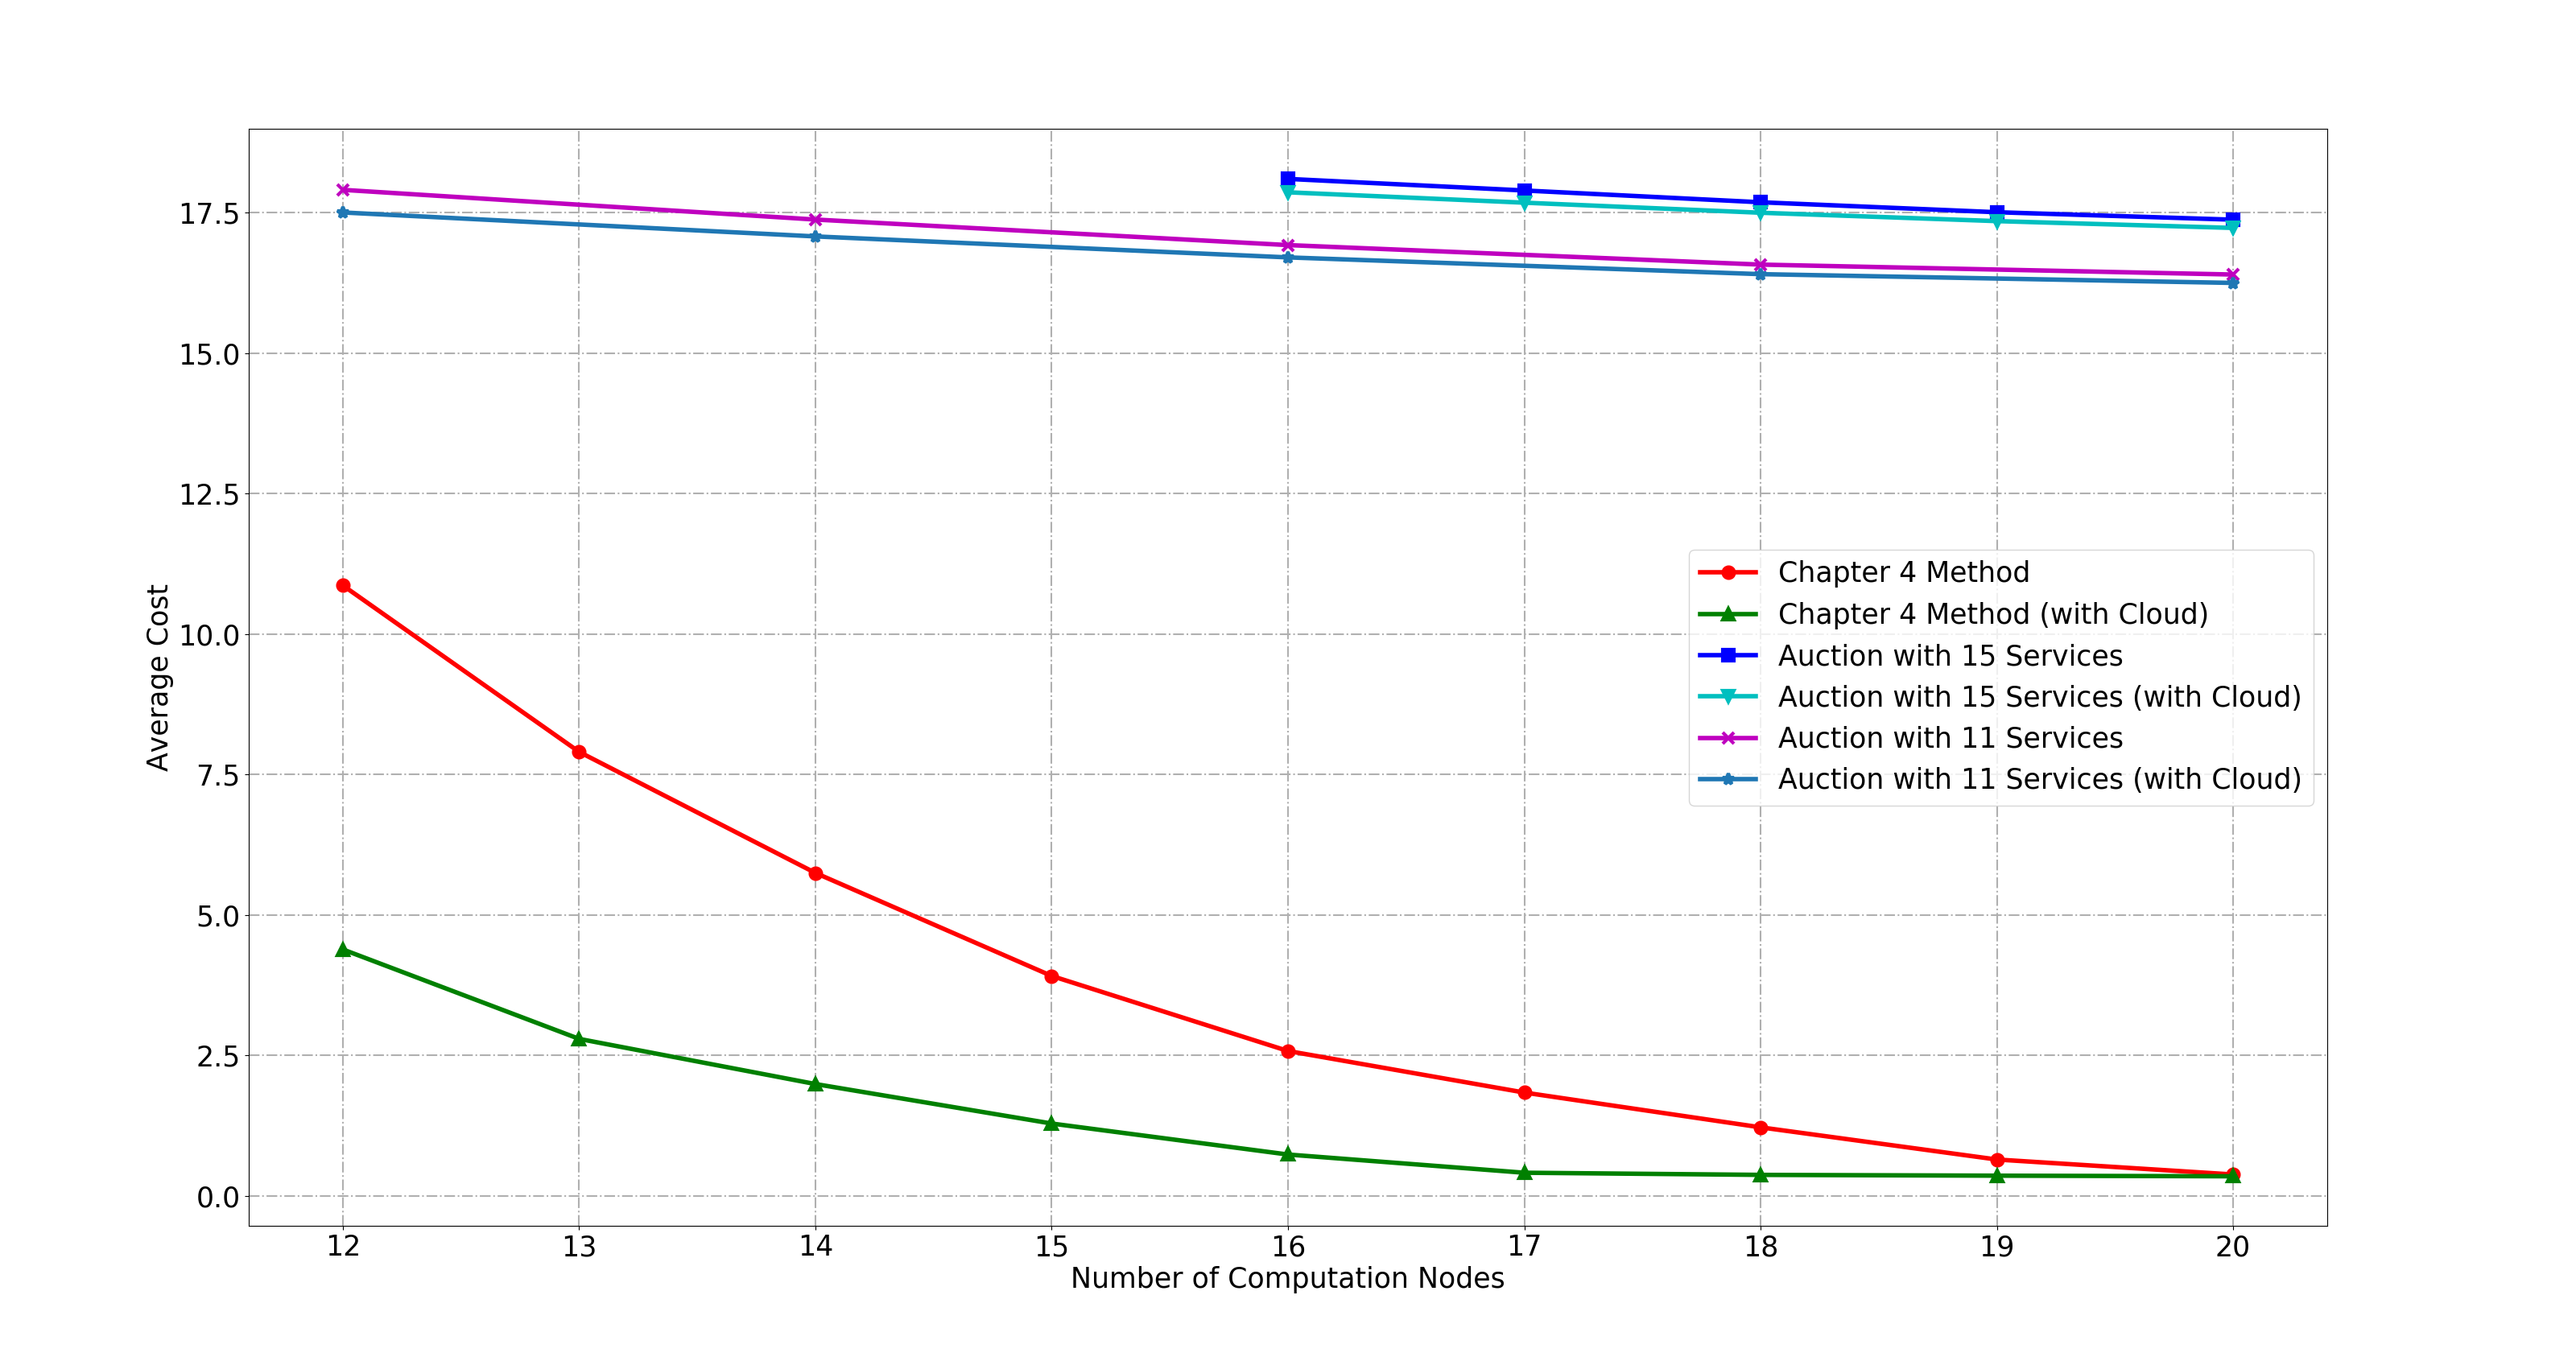
\includegraphics[width=17cm]{graphics/many_to_many/sim_6}}
      \caption{میانگین هزینه سرویس‌ها در برابر تعداد منابع پردازشی در لبه شبکه}
      \label{fig:many_to_many:sim6}
    \end{figure}

    اثر پارامتر $\beta$ در این روش تخصیص منابع در \cref{fig:many_to_many:sim7} بررسی شده‌است.
    در این شکل اثر $\beta$ روی اختلاف نرخ بهینه و مطلوب و بیشترین تاخیر برای یک سرویس در بازه $\beta\in[30, 70]$ رسم شده‌است.
    همان‌طور که بیان شد $\beta$ نسبت اهمیت تاخیر به اختلاف نرخ بهینه و مطلوب است.
    در نتیجه انتظار داریم با افزایش $\beta$ اختلاف نرخ افزایش پیدا کرده و تاخیر کاهش پیدا کند که شکل هم همین را نشان می‌دهد.
    
    \begin{figure}[]
      \centerline{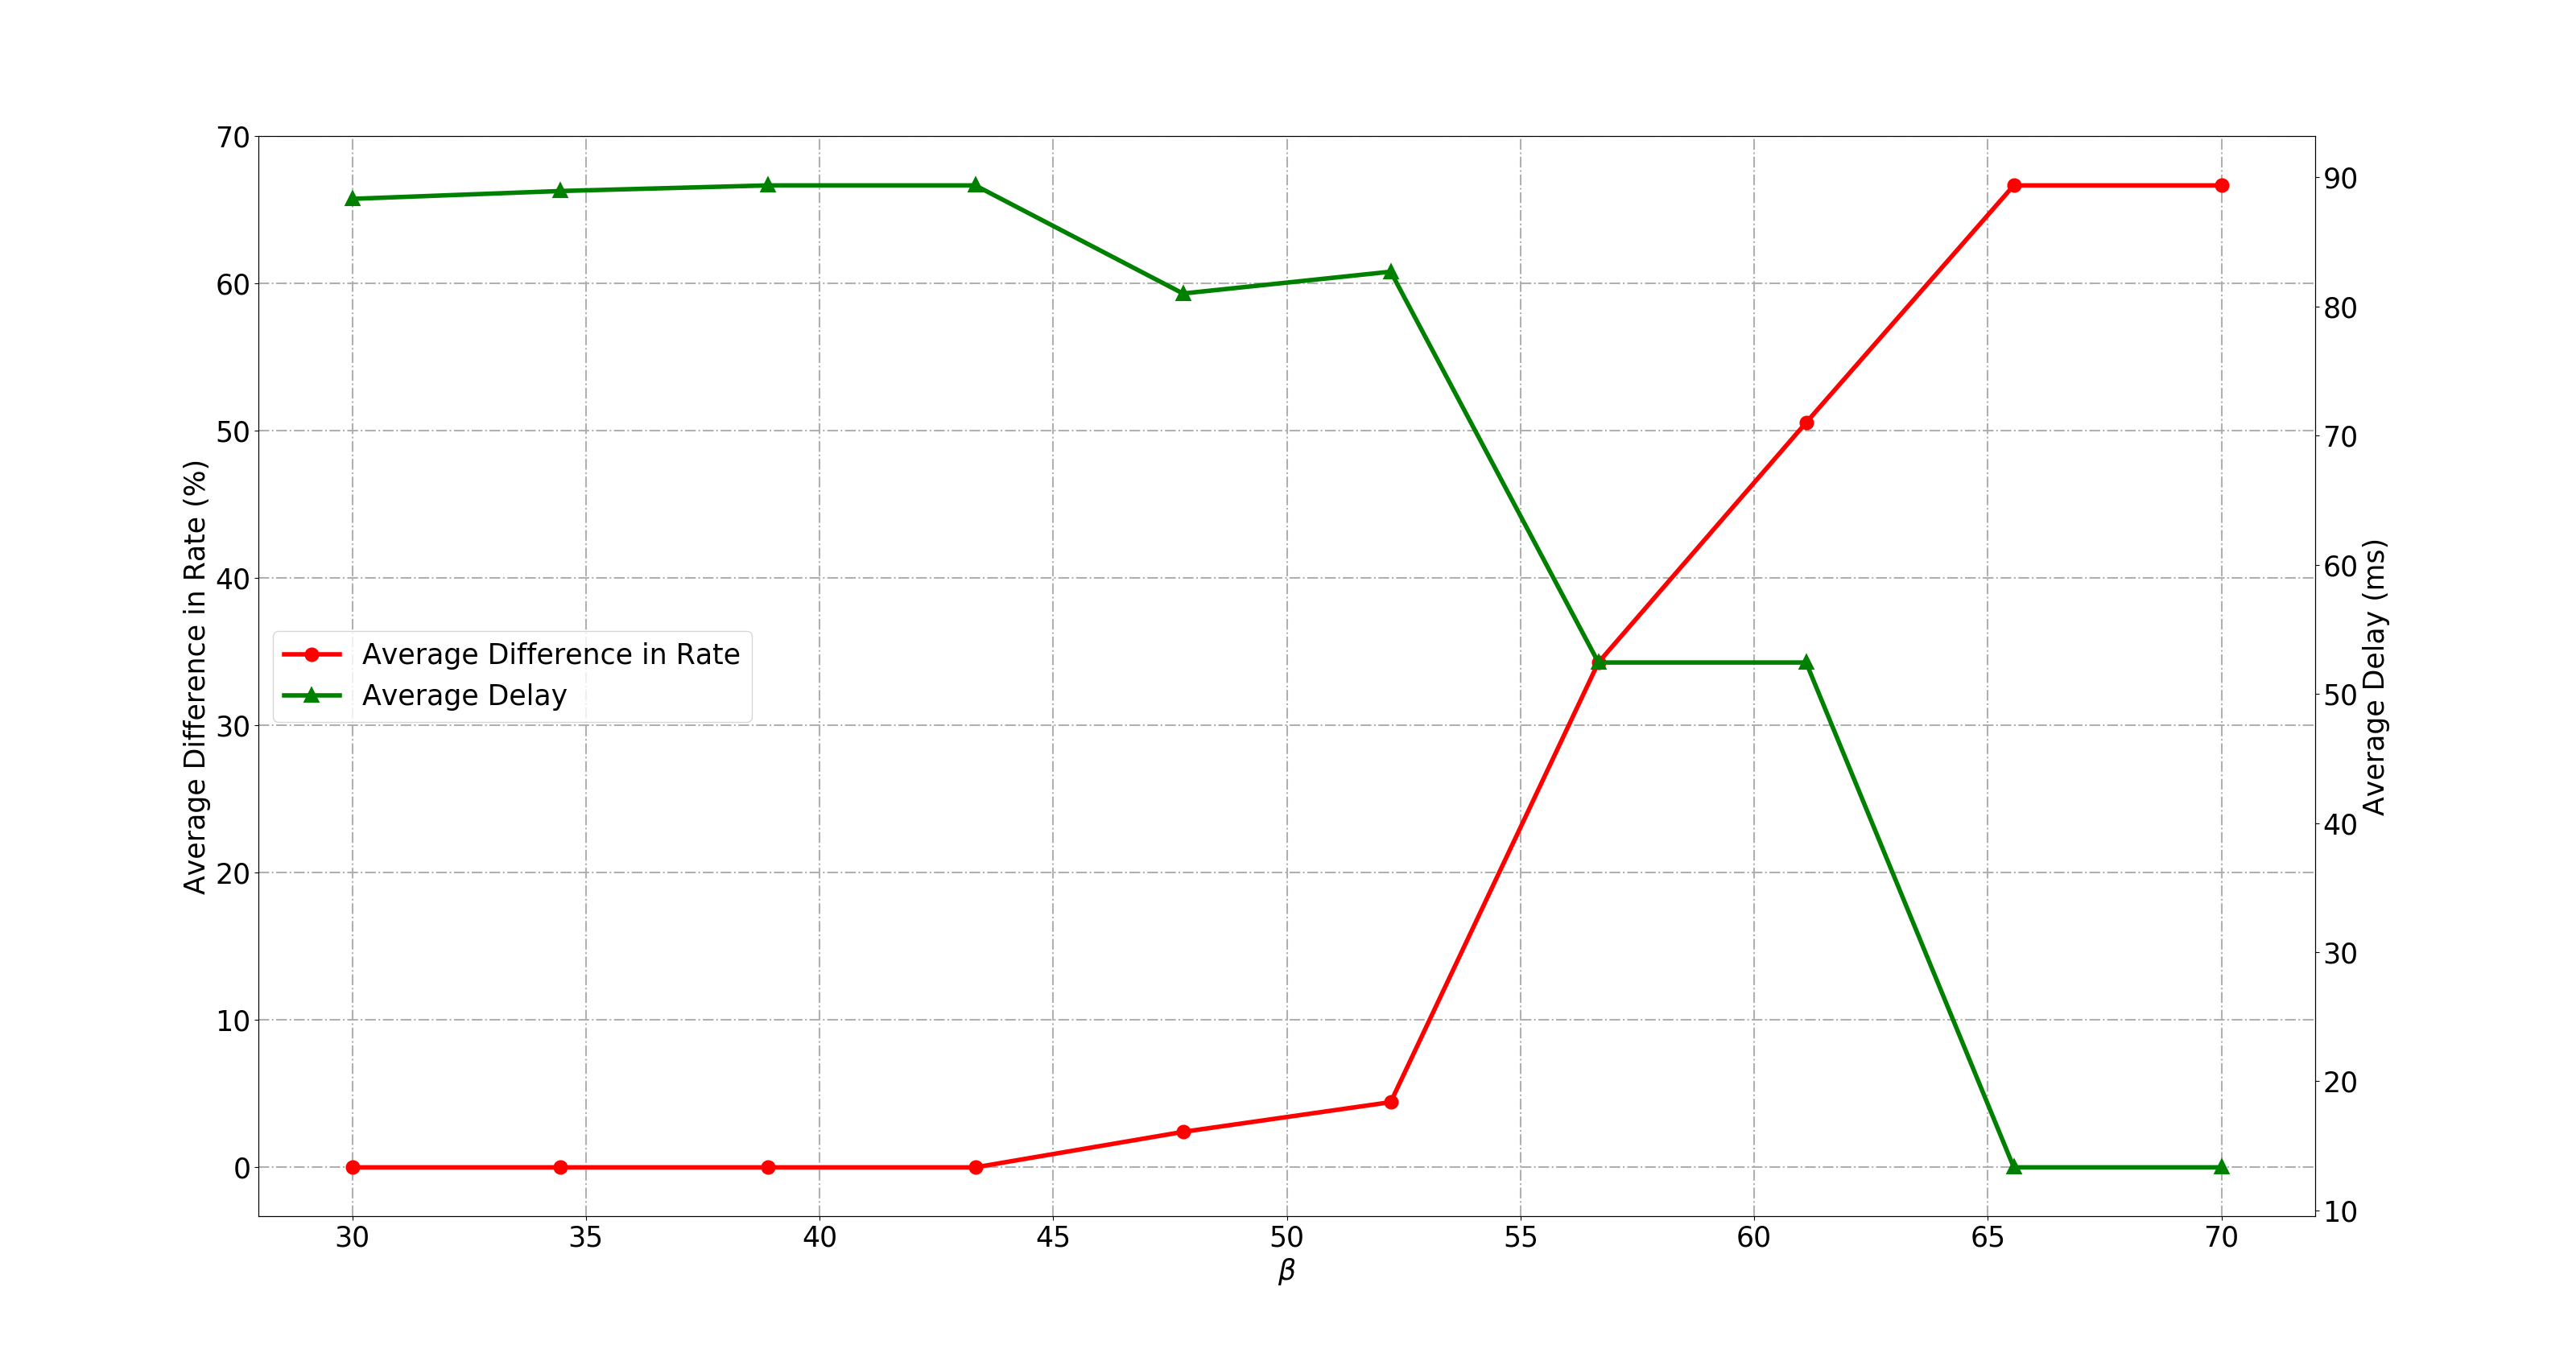
\includegraphics[width=17cm]{graphics/many_to_many/sim_7}}
      \caption{تاثیر $\beta$ بر تاخیر و اختلاف نرخ بهینه با نرخ مطلوب برای یک سرویس}
      \label{fig:many_to_many:sim7}
    \end{figure}

    \begin{figure}[H]
      \centerline{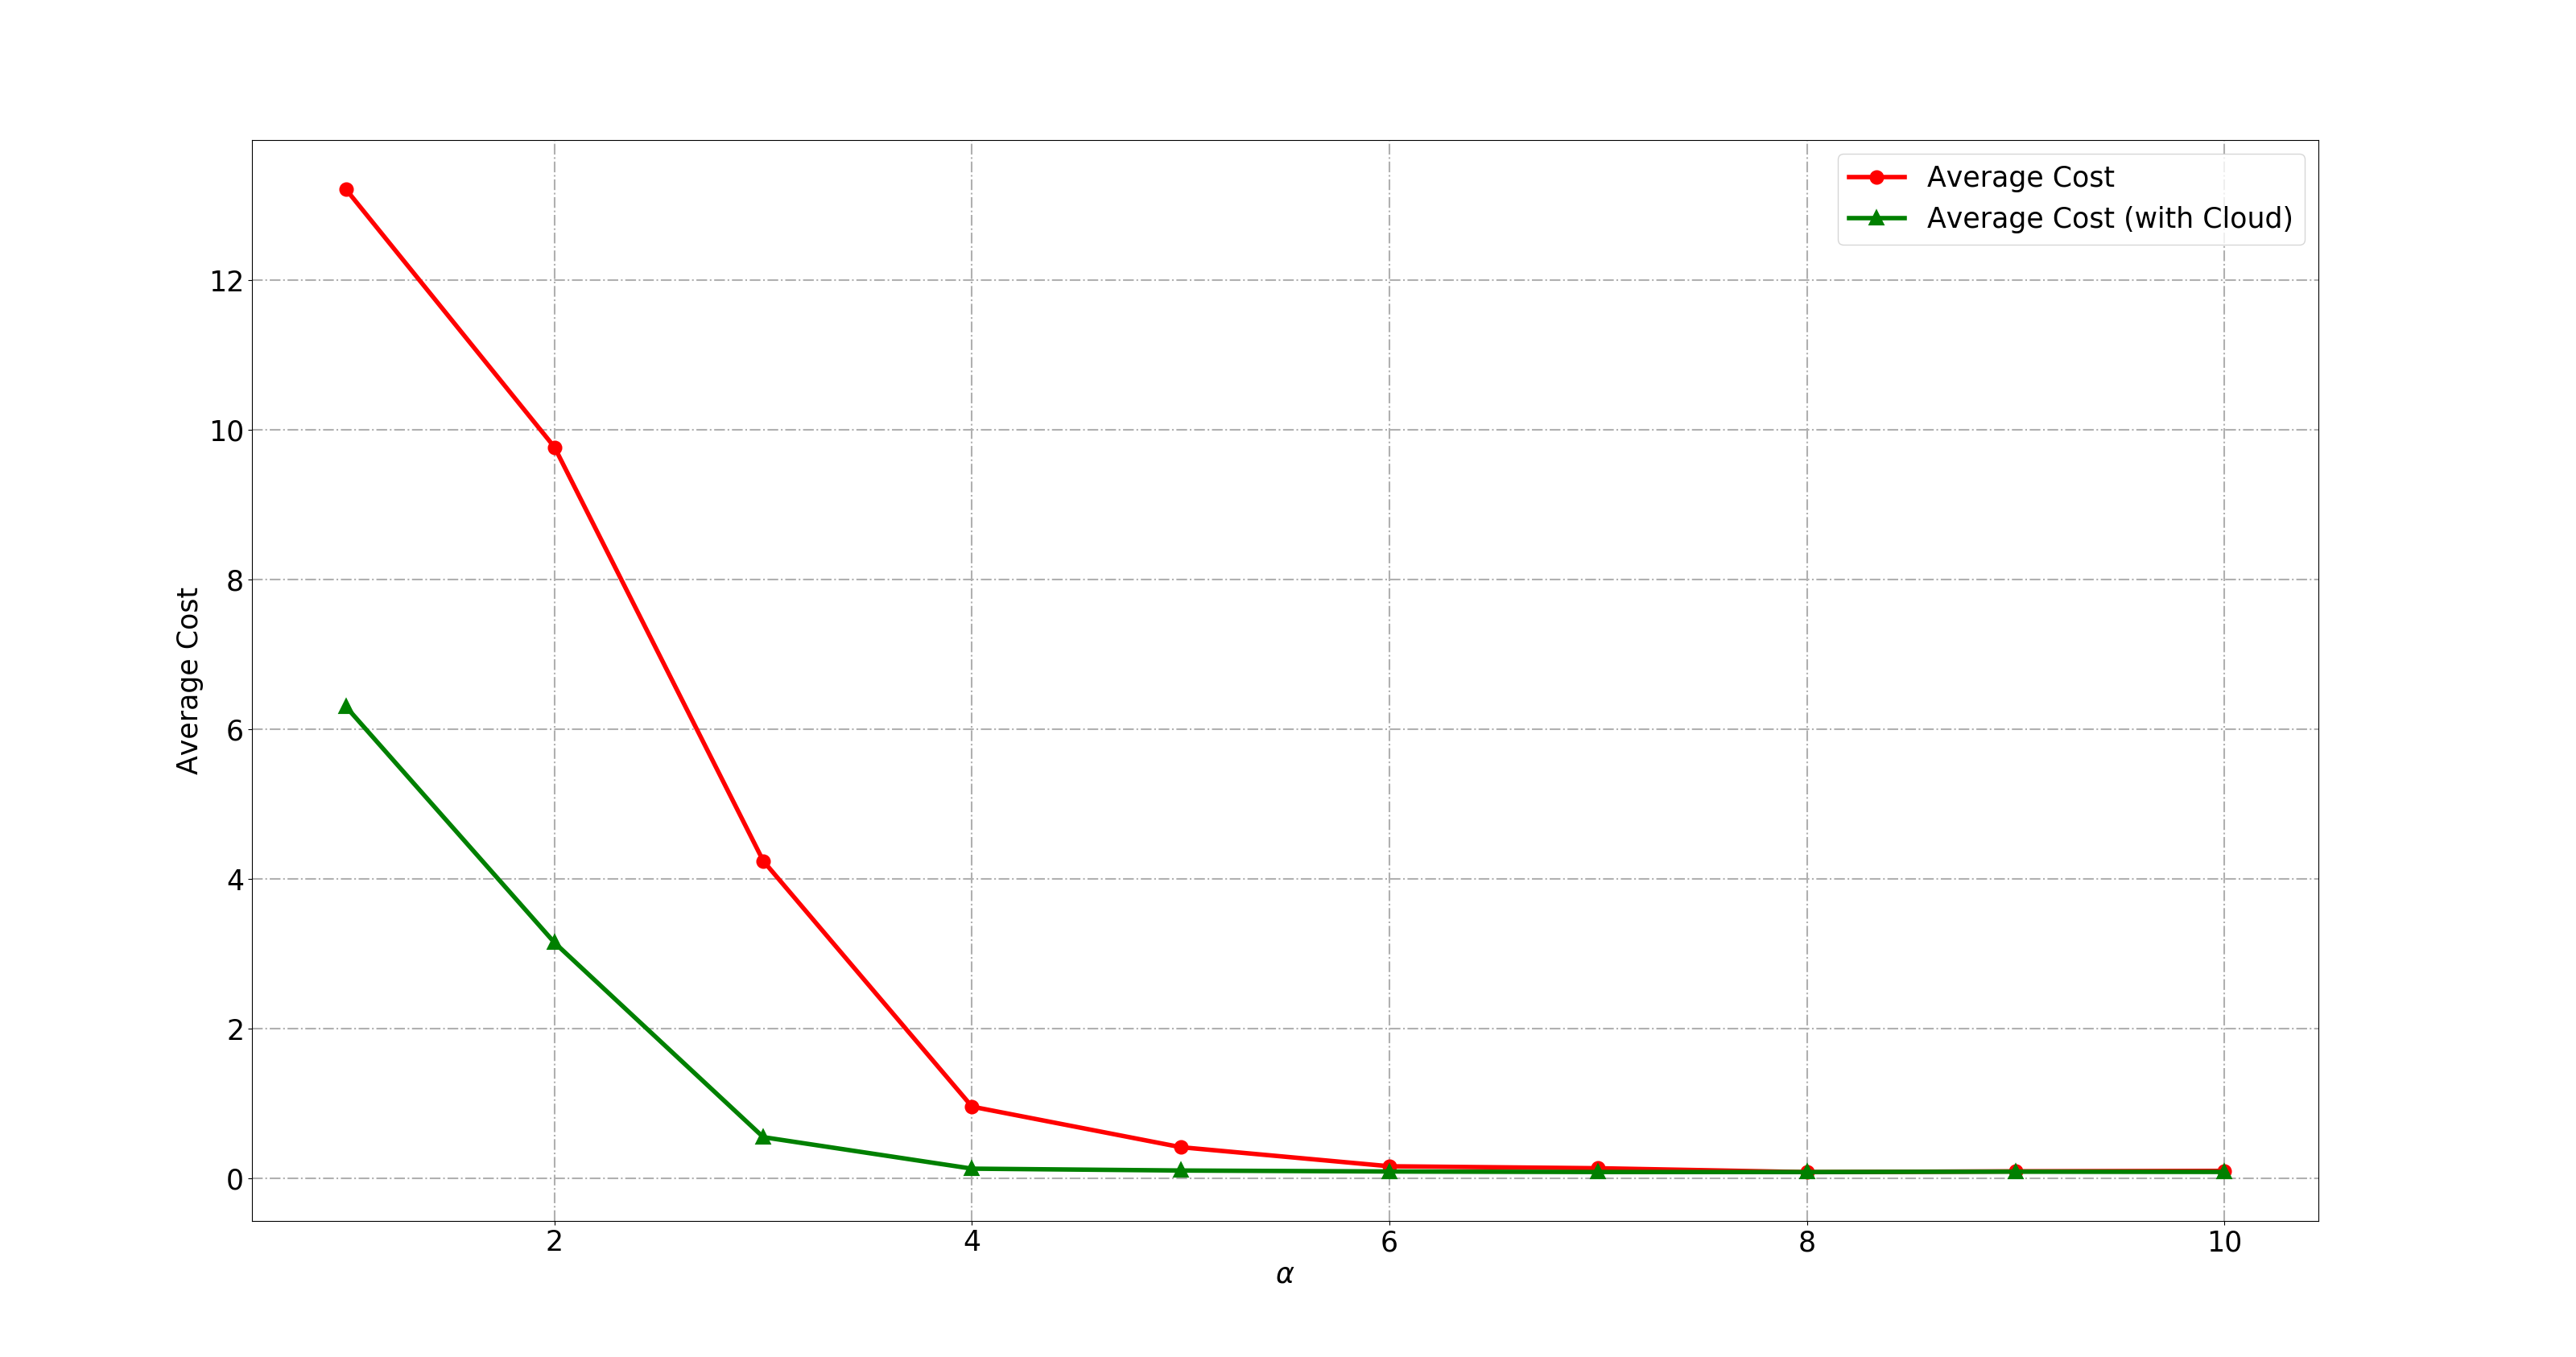
\includegraphics[width=17cm]{graphics/many_to_many/sim_8}}
      \caption{تاثیر $\alpha$ بر میانگین هزینه سرویس‌ها}
      \label{fig:many_to_many:sim8}
    \end{figure}

  \section{جمع‌بندی و نتیجه‌گیری}
    


% مراجع
\pagestyle{empty}
{
\onehalfspacing
\bibliographystyle{ieeetr-fa}%{acm-fa}%{chicago-fa}%{plainnat-fa}%
\bibliography{references}
}

\printindex
% !TeX root=main.tex
% در این فایل، عنوان پایان‌نامه، مشخصات خود و چکیده پایان‌نامه را به انگلیسی، وارد کنید.

%%%%%%%%%%%%%%%%%%%%%%%%%%%%%%%%%%%%

\begin{latin}
  %\latinfaculty{}
  \latindepartment{School of Electrical and Computer Engineering}
  \latinsubject{Electrical Engineering}
  \latinfield{Communication Engineering}
  \latintitle{Virtualized Internet of Things Platform for Smart City Applications}
  \firstlatinsupervisor{Dr. Vahid Shah-Mansouri}
  %\secondlatinsupervisor{Second Supervisor}
  %\firstlatinadvisor{First Advisor}
  %\secondlatinadvisor{Second Advisor}
  \latinname{Ali}
  \latinsurname{Sorour Amini}
  \latinthesisdate{September 2019}
  
  \latinkeywords{Internet of Things (IoT), Smart City, edge computing, resource assignment}
  
  \en-abstract{
    By moving towards the Internet of Things (IoT) era, the number of connected devices to the internet is increasing exponentially.
    Such a large number of devices creates bottlenecks in several areas including device connectivity, data transport, and data processing.
    Edge computing, a computation paradigm trying to process data at the edge of the network, is a promising solution for the processing of the large amount of data produced by this vast number of connected devices.
    Thanks to new advances in the container based virtualization, it is now possible for network gateways and current edge devices to share their extra computation capacity with IoT services for the purpose of data processing.
    Processing tasks of IoT services can be assigned to the edge devices to offload traffic towards the cloud and to reduce the service delay.
    The vast number of these edge devices and services in IoT networks makes the assignment of computing resources to the services a challenging problem.
    In this paper, we mathematically formulate the problem of assignment of computation resources (i.e. edge or cloud) to IoT services in the IoT network.
    The problem is modeled as an optimization problem with the objective of maximizing the total utility of the services.
    The resulting optimization problem is a mixed integer non-linear program which is generally hard to solve.
    Proposed algorithms result in near optimal solutions and well suited for distributed and asynchronous deployment.
  }

  \cleartoleftpage
  \latinabstractPage
  \cleartoleftpage
  \latinfirstPage
\end{latin}

\label{LastPage}

\end{document}
